\documentclass[10pt,twoside,openright]{book}
\usepackage[utf8]{inputenc}
\usepackage[spanish,english]{babel}
\usepackage[sc]{mathpazo}
\linespread{1.05}
\usepackage[T1]{fontenc}
\usepackage{xcolor}
\definecolor{aaublue}{RGB}{33,26,82}% dark blue
\usepackage{graphicx}
\usepackage{epstopdf}
\usepackage{caption}
\captionsetup{%
	font=footnotesize,
	labelfont=bf 
}
\usepackage{array,booktabs}
\usepackage{tabularx}
\usepackage{multirow}
\usepackage{framed}
\usepackage{tikz,pgfplots}
\usepackage{paralist}
%%%%%%%%%%%%%%%%%%%%%%%%%%%%%%%%%%%%%%%%%%%%%%%%
% Mathematics
% http://en.wikibooks.org/wiki/LaTeX/Mathematics
%%%%%%%%%%%%%%%%%%%%%%%%%%%%%%%%%%%%%%%%%%%%%%%%
\usepackage{amsmath}
\usepackage{amsthm}
\usepackage{amssymb}
\usepackage{proba}
\usepackage{breqn}
\usepackage{framed}
%\usepackage[framed,amsmath,amsthm,thmmarks]{ntheorem}
\usepackage[
	paperwidth= 21.59cm,
	paperheight=27.94cm,
	%width = 15.5cm
	%left=1.0in,
	right=1.0in,
	%top=1in,
	%bottom=1in
	%outer=4.75cm,
	%inner=4.75cm,
	%top=2.5cm,
	%bottom=2.5cm
	]{geometry}
\usepackage{bigints}
\usepackage{physics}
%\usepackage{thm-tools}

%\renewcommand{\thesection}{\arabic{section}}
%\usepackage{titlesec}
%	\titleformat*{\section}{\normalfont\Large\bfseries\color{aaublue}}
%	\titleformat*{\subsection}{\normalfont\large\bfseries\color{aaublue}}
%	\titleformat*{\subsubsection}{\normalfont\normalsize\bfseries\color{aaublue}}
%\titleformat*{\paragraph}{\normalfont\normalsize\bfseries\color{aaublue}}
%\titleformat*{\subparagraph}{\normalfont\normalsize\bfseries\color{aaublue}}
% Change some default names
\addto\captionsenglish{%this line is required when using the babel package
	\renewcommand\bibname{References} % change Bibliography to references
	\renewcommand\figurename{Figure} % change Figure to Fig.
}
\usepackage[page, title, titletoc]{appendix}
\usepackage{fancyhdr}
	\pagestyle{fancy}
	\fancyhf{} %delete everything
	\renewcommand{\headrulewidth}{1pt} %remove the horizontal line in the header
	\fancyhead[RE]{\color{aaublue}\small\nouppercase\leftmark} %even page - chapter title
	\fancyhead[LO]{\color{aaublue}\small\nouppercase\rightmark} %uneven page - section title
	\fancyfoot[CE,CO]{\thepage} %page number on all pages
	\raggedbottom
\usepackage{calc}
\usepackage{enumerate}
%\usepackage{mparhack}
%\usepackage{bibunits}
%\usepackage[sectionbib]{chapterbib}
% Custom bibliograhy - used in the list of papers
%\usepackage{multibib}
%\newcites{main}{Main References}
%\newcites{other}{Other Publications}
% Change [1,2,3,4] into [1-4]
%\usepackage{cite}
\usepackage[square,sort,comma,numbers]{natbib}
%%%%%%%%%%%%%%%%%%%%%%%%%%%%%%%%%%%%%%%%%%%%%%%%
% Misc
%%%%%%%%%%%%%%%%%%%%%%%%%%%%%%%%Dynamical Systems and Numerical Analysis%%%%%%%%%%%%%%%%
% Add bibliography and index to the table of
% contents
\usepackage[nottoc,section]{tocbibind}
% Enable subappendices
\usepackage{appendix}
\renewcommand{\setthesection}{\Alph{section}} % remove the chapter numbering
\usepackage{lastpage}
\usepackage[
%  disable, %turn off todonotes
	colorinlistoftodos, %enable a coloured square in the list of todos
	textwidth=2cm, %set the width of the todonotes
	textsize=scriptsize, %size of the text in the todonotes
	]{todonotes}
\setlength{\marginparwidth}{2cm}
\setlength{\parindent}{15pt}
\usepackage{hyperref}
\hypersetup{%
	plainpages=false,%
	pdfauthor={Author},%
	pdftitle={Title},%
	pdfsubject={Subject},%
	bookmarksnumbered=true,%
	colorlinks=true,%
	citecolor=aaublue,%
	filecolor=aaublue,%
	linkcolor=aaublue,% you should probably change this to black before printing
	urlcolor=aaublue,%
	pdfstartview=FitH%
	linktocpage=true,%
}
\usepackage{cleveref}
\usepackage{siunitx}
\usepackage{subfig}
\usepackage{thmtools}
\usepackage{xspace}
\usepackage{import}
% see, e.g., http://en.wikibooks.org/wiki/LaTeX/Formatting#Hyphenation
% for more information on word hyphenation
\hyphenation{ex-am-ple hy-phen-a-tion short}
\hyphenation{long la-tex}

 
%\theoremheaderfont{\normalfont\bfseries}
%\theorembodyfont{\normalfont}
%\theoremstyle{break}
%\def\theoremframecommand{{\color{aaublue!50}\vrule width 5pt \hspace{5pt}}}
%\newcommand{\includepaper}[1]{
	%\cleardoublepage
	%\setcounter{enumiii}{0}
	%\setcounter{enumii}{0}
	%\setcounter{enumiv}{0}
	%\setcounter{enumi}{0}
	%\setcounter{equation}{0}
	%\setcounter{figure}{0}
	%\setcounter{footnote}{0}
	%\setcounter{lofdepth}{1}
	%\setcounter{lotdepth}{1}
	%\setcounter{mpfootnote}{0}
	%\setcounter{paragraph}{0}
	%\setcounter{parentequation}{0}
	%\setcounter{part}{0}
	%\setcounter{section}{0}
	%\setcounter{subfigure}{0}
	%\setcounter{subparagraph}{0}
	%\setcounter{subsection}{0}
	%\setcounter{subsubsection}{0}
	%\setcounter{subtable}{0}
	%\setcounter{table}{0}
	%\include{#1}
%}
\newenvironment{abstract}{\section*{Abstract}\it}{}
\DeclareMathAlphabet{\mathpzc}{OT1}{pzc}{m}{it}
\theoremstyle{definition}
\newtheorem{definition}{Definition}[section]
\newtheorem{dfn}{Definition}[section]
\newtheorem{assumption}{Assumption}[section]
\newtheorem{hypothesis}{Hypothesis}[section]
%
\theoremstyle{plain}% default
\newtheorem{thm}{Theorem}[section]
\newtheorem{pro}{Proposition}[section]
\newtheorem{lem}{Lemma}[section]
\newtheorem{corollary}{Corollary}[section]
\newtheorem{consequence}{CONSEQUENCE}[section]
\theoremstyle{remark}
\newtheorem{remark}{Remark}[section]
\newtheorem{pf}{Proof}
\newtheorem{Proof}{Proof}[]
\theoremstyle{definition}
\newtheorem{example}{Example}[section]
%declaration theorems for appendix
\declaretheorem[numbered=no, name=H\"{o}lder]{Holder}
\declaretheorem[numbered=no, name=Young]{Young}
\declaretheorem[numbered=no, name=Minkowski]{Minkowski}
\declaretheorem[numbered=no, name=Doob's Martingale Inequality]{Doobs}
\declaretheorem[numbered=no, name=Burkholder–Davis–Gundy inequality]{bdg}
\declaretheorem[numbered=no, name=Gronwall inequality]{Gronwall}
\declaretheorem[numbered=no, name=Discrete Gronwall Inequality]{DiscreteGronwall}
\declaretheorem[numbered=no, name=A standard inequality]{Standard}
\makeatletter
	\@addtoreset{equation}{section}
\makeatother
%
\providecommand*{\lemautorefname}{Lemma}
\providecommand*{\thmautorefname}{Theorem}
\providecommand*{\assumptionautorefname}{Assumption}
\providecommand*{\hypothesisautorefname}{Hypothesis}
%
\newcommand{\normL}[1]{\left[\mathbb{E}\left|#1\right|^2\right]^{1/2}}
\newcommand{\ms}[1]{\mathbb{E}\left|#1\right|^2}
\newcommand{\mep}[1]{\mathbb{E}|#1|^p}
\newcommand{\m}[1]{\mathbb{E}#1}
\newcommand{\meanp}[2]{\mathbb{E}\left|#1\right|^{#2}}
\newcommand{\condexp}[2]{\mathbb{E}\left[#1|#2\right]}
\newcommand{\lftrght}[3]{\left#2 #1\right #3}
\newcommand{\revision}[1]{\textcolor{BrickRed}{#1}}
\crefrangeformat{equation}{(#3#1#4)--(#5#2#6)}
\newcommand{\innerprod}[2]{\left\langle#1, #2\right\rangle}
\newcommand{\Prob}[1]{\mathbb{P}\left[#1\right]}
\newcommand*{\eg}{e.g.,\xspace}
\newcommand*{\ie}{i.e.,\xspace}
\newcommand{\SM}{LS \xspace}
\DeclareMathOperator{\diag}{diag}
\DeclareMathOperator*{\as}{a.s.}
%\DeclareMathOperator{\Tr}{Tr}
\newcommand{\crefrangeconjunction}{--}
\crefrangeformat{equation}{(#3#1#4)--(#5#2#6)}
\crefname{hypothesis}{hypothesis}{hypotheses}
\Crefname{hypothesis}{Hypothesis}{Hypotheses}
%
%%%%%%%%%%%%%%%%%%%%%%%%%%%%%%%%%%%%%%%%%%%%%%%%
% Various names
%%%%%%%%%%%%%%%%%%%%%%%%%%%%%%%%%%%%%%%%%%%%%%%%
\newcommand{\IEEEPARstart}[2]{#1#2}
%%%%%%%%%%%%%%%%%%%%%%%%%%%%%%%%%%%%%%%%%%%%%%%%
% Bibliography
%%%%%%%%%%%%%%%%%%%%%%%%%%%%%%%%%%%%%%%%%%%%%%%%
\newcommand{\defaultbibA}{%
	\bibliographystyle{elsarticle-num}
	\bibliography{bib/Bibliography}
}
\newcommand{\defaultbibB}{%
	\bibliographystyle{elsarticle-num}
	\bibliography
}% 
\begin{document}
%frontmatter
	\frontmatter
	\pagestyle{empty} 
	\pagenumbering{roman}
	\pdfbookmark[0]{Front page}{label:frontpage}%
\begin{titlepage}
	\addtolength{\hoffset}{0.5\evensidemargin-0.5\oddsidemargin}
  %set equal margins on the frontpage - remove this line if you want default margins
	\noindent%
	\begin{tabular}{@{}p{\textwidth}@{}}
		\toprule[2pt]
		\midrule
		\vspace{0.2cm}
		\begin{center}
			\Huge{\textbf{
					Steklov Methods for Nonlinear Stochastic Differential Equations.
				}
			}
		\end{center}
		\vspace{0.2cm}\\
		\midrule
		\toprule[2pt]
	\end{tabular}
	\vspace{3 cm}
	\begin{center}
		{
			\large
				Ph.D. Dissertation%Insert document type (e.g., Project Report)
		}\\
		\vspace{0.2cm}
		{
			\Large
			Sa\'ul D\'iaz Infante Velasco.
		}
		\end{center}
		\begin{center}
			
\includegraphics{frontmatter/Logo}
		\end{center}

		\vfill
	\begin{center}
		Dissertation submitted \today
	\end{center}
	\end{titlepage}
	\clearpage

	\thispagestyle{empty}
\noindent
\begin{tabularx}{\textwidth}{@{}lX}
    Thesis submitted:	& \today\\
    PhD Supervisor:		& Prof.\ Silvia Jerez\\
					    & CIMAT A.C.\\
    PhD Committee:		& Prof.\ Rolando Biscay, CIMAT, Guanajuato. \\
					    & Prof.\ Gilberto Carlos Gonzalez Parra,
					    University of Los Andes, Venezuela\\						
						& Prof.\ Ram\'on Casta\~{n}eda Priego, University of Guanajuato.\\
						& Prof.\ Moises Santill\'an Zer\'on, CINVESTAV Monterrey. \\
						
						
\end{tabularx}
\strut\vfill
\noindent
	\noindent Published by:\newline
	CIMAT A.C. \newline
	Calle Jalisco sn\newline
	Guanajuato, Gto.\newline
	Phone: +45 99407140\newline
	sauld@cimat.mx\newline
	\strut\vfill
	\noindent \copyright{} Copyright by author\newline
	\strut\vfill
	\noindent Printed in CIMAT A.C. 
	\strut\vfill\vfill\vfill
	\clearpage


	%\chapter*{Curriculum Vitae\markboth{Curriculum Vitae}{Curriculum Vitae}}\label{ch:cv}
	\pagestyle{fancy}
	\addcontentsline{toc}{chapter}{Curriculum Vitae}
	\begin{tabularx}{\textwidth}{@{}Xr}
		\Large Sa\'ul D\'iaz Infante Velasco & 
	\raisebox{-\totalheight/2}{\includegraphics[width=2cm]{frontmatter/cvPicture.png}}\\
	\end{tabularx}\par
	\vspace{0.5cm}\noindent
	Here is the CV text.

	\chapter*{Abstract\markboth{Abstract}{Abstract}}\label{ch:Abstract}
	\addcontentsline{toc}{chapter}{Abstract}
	
	
	
	
	
	
	In this paper, we develop a new  numerical method with asymptotic stability
	properties for solving stochastic differential equations (SDEs).  Foundations
	for the  new  solver are the Steklov mean and an exact discretization for the
	deterministic version of  the SDEs. Strong consistency and  convergence properties are
	demonstrated for the proposed  method. Moreover, a rigorous  linear and nonlinear
	asymptotic stability analysis  is  carried out for the multiplicative case in a
	mean-square sense and  for the additive case  in a path-wise sense using the pullback
	limit. In order to emphasize characteristics  of the Steklov discretization  we
	use as benchmarks the stochastic logistic equation  and  the Langevin equation with a
	nonlinear potential of the Brownian dynamics. We show that  the Steklov method has
	mild stability requirements and allows long-time simulations in  several applications.
	

	\cleardoublepage
	\pdfbookmark[0]{Contents}{label:contents}
	\pagestyle{fancy}
	\tableofcontents
	\listoffigures
	\listoftables
	%\listoftodos
	\chapter*{
	Thesis Details
		\markboth{Thesis Details}{Thesis Details}
	}
	\addcontentsline{toc}{chapter}{Thesis Details}
%this is a mandatory page. You can see more at http://www.phd.teknat.aau.dk/intranet/templates/
\begin{tabularx}{\textwidth}{@{}>{\bfseries}l X@{}}
	Title:			& Steklov Methods for non Linear Stochastic Differential
					Equations.\\
	Ph.D. Student:	& Sa\'ul D\'iaz Infante Velasco.\\
	Supervisor:		& Prof.\ Silvia Jerez Galiano, CIMAT A.C.\\
\end{tabularx}
\vspace{\baselineskip}

% list the papers included in this thesis
\noindent The main body of this thesis consist of the following papers.
\begin{itemize}
  \item[{[\ref{paper:paperA}]}] Sa\'ul D\'iaz-Infante, Silvia Jerez
  "Convergence and asymptotic stability  of  the explicit Steklov method for stochastic differential 
	equations,'' \emph{Journal of Computational and Applied Mathematics}\\ 
	DOI: 10.1016/j.cam.2015.01.016 14-FEB-2015
	vol.~291, pp. 36-47, 2015.
  \item[{[\ref{paper:paperB}]}] Sa\'ul D\'iaz-Infante, Silvia Jerez,
	The Linear Steklov Method for SDEs with non-globally Lipschitz
	Coefficients: Strong convergence and simulation. Paper submitted at
	\emph{Journal of Computational and Applied Mathematics.}
	
\end{itemize}
\noindent This thesis has been submitted for assessment in partial fulfillment of the PhD degree. The thesis is based 
on the submitted or published scientific papers which are listed above. Parts of the papers are used directly or 
indirectly in the extended summary of the thesis. As part of the assessment, co-author statements have been made 
available to the assessment committee and are also available at the Faculty. 
	\cleardoublepage
%mainmatter
	\mainmatter
	\chapter{Introduction and main results}
		\label{ch:Chapter1}
		\section{Introduction}
	In the last decades, stochastic differential modeling has become a rapidly-growing research area. Historically, it 
	appeared as an extension of the deterministic differential modeling of over-idealized situations with fluctuating 
	behavior of the analyzed physical phenomenon.  Actually, it is an important research area by itself that describes 
	important phenomena such as turbulent diffusion, spread of diseases, genetic regulation, motion of 
	particles etc. \cite{Allen2007, Gardiner2009, VanKampen1992}. 

		We can obtain the explicit solution of only few SDEs, therefore developing accurate stochastic
	numerical approximations represent  an option to analyze and confirm (by simulation) the nature of a 
	stochastic model. Stochastic numerics allow the  analysis of some  model properties that are
	difficult or impossible to measure experimentally in laboratories, for example its
	long-time behavior. In this cases, we require that a numerical solvers
	be able to reproduce asymptotic behavior like mean square stability \cite{Higham2000,Higham2000b,Saito1996a},
	usually, a linear  analysis can be considered as the first step for understanding a method, but it is not 
	an indicator of qualitative behavior on the nonlinear case \cite{kloeden1999towards}. Thus, some theoretical 
	work on asymptotic	stability has appeared for nonlinear SDEs \citet{Bokor2003} \citet{Buckwar2011a}.  
	
		The first methods for solving SDEs were stochastic extensions of deterministic algorithms,
	for example schemes as the Euler-Maruyama, Taylor and Runge-Kutta \cite{Bokor2003,Burrage2004, Kloeden1992}.
	Unfortunately, sometimes their asymptotic stability conditions are very restrictive, considers for
	example the Brownian Dynamics Simulations, here the Euler-Maruyama discretization is the standard method to 
	solve the Langevin equation that describe the motion of particles \cite{Braanka1998, Bussi2007, Ermak1978}. 
	However, the operation time step size of this scheme has to be pint-size, otherwise the scheme becomes unstable. 
	Now, the construction of methods focus on structural or dynamic properties of a specific SDE.
	Some examples are the balanced methods for stiff SDE \cite{Milstein1998a} the quasi-symplectic schemes for
	stochastic Hamiltonian systems \cite{Milstein2003} and SDEs with small noise \cite{Buckwar2006b}.
	
		Numerical convergence and stability are well understood for SDE with globally Lipschitz 
	continuous coefficients, which discard  many important models from applications.
	Moreover, \citeauthor*{Hutzenthaler2009} report in \cite{Hutzenthaler2009} that if a SDE
	has drift or diffusion,	which grows faster that a linear function, then the EM diverges in strong and weak sense.
	This result opens a new chapter on the design of numerical methods ---
	stochastic models in applications as Finance, Biology and Physics use SDEs with locally Lipschitz 
	coefficients. In addition, \citeauthor*{Giles2008} proposes in \cite{Giles2008} a new variance reducing technique
	that relies in strong numerical convergence, which optimizes the traditional Monte Carlo simulation. Thus, 
	developing	explicit schemes, which converges in strong sense with super-linear coefficients attracts the right 
	now attention.
	
		Recently research has been focused on modifying the EM method to obtain strong convergence  under 
	the previous conditions keeping its simple structure and  its low computational cost. Several methods have been 
	developed in this direction:  the family of  Tamed schemes
	\cite{Hutzenthaler2012a, Wang2011, Zong2014,Hutzenthaler2015}, 
	a special type of balanced method \cite{Tretyakov2013},  the stopped scheme \cite{Liu2013a} .
	For SDE with super-linear diffusion, \citeauthor{Mao2013a} provided results
	for the strong convergence of implicit methods as the Backward-Euler-Maruyama. However, the convergence of explicit 
	schemes for SDEs with super-linear growth is still under development. Works on this subject  are
	\citeauthor{Mao2015} \cite{Mao2015} with the truncated Euler method and \cite{Sabanis2015} with a new kind of
	tamed scheme. There, the strong convergence of the proposed method
	is proved using the theory developed by in \citet*{Higham2002b} or by means of  the new 
	approach given by  \citet{Hutzenthaler2015}.
	Both techniques prove strong convergence by verifying boundedness moments of the numerical and 
	analytical solution of the underlying SDE. In spite of the recent work in this subject,  it is still necessary
	to get more accurate numerical methods for SDE under super-linear growth and 
	non-globally Lipschitz coefficients.

\section{Main Results}
		Our main contribution follows two lines of research. The first one is to design an explicit numerical
	scheme with good stability properties. We focus on explicit methods because we are interested on applications of 
	Brownian Dynamics, so we seek a simple and fast numerical solver. Also we require a stable scheme 
	in order to obtain  simulations for long periods of time. For example in Brownian Dynamics, the self-diffusion
	coefficient is an asymptotic property. We propose the Steklov method, which is a stochastic 
	extension of an exact deterministic numerical scheme. 
		
		The second line consists in generalize the above scheme to a multidimensional setup and with more general 
	coefficients. Thus, we propose the Linear Steklov (LS) scheme. This explicit method is based on  a linear version 
	of the Steklov average with a split-step formulation. We prove for this scheme a one-half 
	convergence order with a one sided Lipschitz condition and polynomial growth on the drift; and a globally 
	Lipschitz condition on the diffusion. Also we provide numerical evidence that this method is suitable for problems 
	with super-linear growth diffusion  where other methods have failed. 
	 
\section{Methodology}
		
	\subsection*{Chapter 2 --- Preliminaries}
			
			After the above introduction, in this chapter  we present an overview of basic results from probability 
		theory that we will need in order in order to set our framework.
		Next we state useful concepts and theorems from stochastic process and stochastic  calculus. 
		Finally, we give some important qualitative properties of numerical methods for stochastic differential 
		equations.
	
	\subsection*{Chapter 3 --- Steklov method for scalar SDEs with Globally Lipschitz coefficients}
	
			The chapter contains our first contribution ---the Steklov method. 
		First we develop a new numerical method with asymptotic stability properties for solving stochastic 
		differential equations (SDEs). The foundations for the new solver are the Steklov mean and an exact 
		discretization for the deterministic version of the SDEs. Second strong consistency and convergence properties 
		are demonstrated for the proposed method. Moreover, a rigorous linear and nonlinear asymptotic stability 
		analysis is carried out for the multiplicative case in a mean-square sense and for the additive case in a 
		path-wise sense using the pullback limit. In order to emphasize the characteristics of the Steklov 
		discretization we use as benchmarks the stochastic logistic equation and the Langevin equation with a nonlinear 
		potential of the Brownian dynamics. We show that the Steklov method has mild stability requirements and allows 
		long-time simulations in several applications.
	
	\subsection*{Chapter 4 --- Steklov Method for SDEs with Non-Globally Lipschitz Continuous Drift}
	
			In this chapter we present an explicit numerical method for solving stochastic differential equations with
		non-globally Lipschitz coeffcients. A linear version of the Steklov average under a split-step formulation 
		supports our new solver. The Linear Steklov method converges strongly with a standard
		one-half order. Also, we present numerical evidence that the explicit Linear Steklov reproduces almost surely 
		stability solutions with high-accuracy for diverse application models even
		for stochastic differential systems with super-linear diffusion coefficients.
		
	
	\subsection*{Chapter 5 --- Conclusions and future work}
	
			Finally, in this Chapter  we restate our contribution followed by conclusions and discuss 
		possible future directions for our research.
	\chapter{Preliminaries}
		\label{ch:Chapter2}
			Here we present some results from stochastic analysis. This chapter focus on
provide the basic information and tools to understand the nature of a SDE and its numerical approximation. For reference
see \cite{Arnold1979, Kloeden1992, Williams1991, Milstein2004, Resnick2003}.

\section{Probability theory and Stochastic Processes}
		Probability theory  is the field that  studies the random phenomena. A random event is the set of  outcomes from an 
experiment conducted under the same conditions  with a variability in results . Probability theory aims to 
describe  this variability. We denote by $\Omega$ the set of observable outcomes, $\omega$, from a
experiment or phenomenon.  However, not every observable event is measurable, so  for the purpose of probability 
theory, a family of subsets from $\Omega$ with particular properties  a ---$\sigma$-algebra is needed. In 
the following, we formalize these concepts, for reference see e.g. \cite{Resnick2003}.	
\begin{definition}[$\sigma$-algebra]
	Let $\Omega$ a set and $\calF$ a family of subset of $\Omega$, we call $\calF$ a 
	$\sigma$- algebra if the following properties hold:
	\begin{enumerate}[(i)]
		\item $\emptyset \in \calF$,
		\item if $F\in \calF$ then $F^c\in\calF$ where $F^c = \Omega \setminus F$,
		\item if $\displaystyle \{F_i\}_{i=1}^\infty \in \calF $ then 
			$\displaystyle \bigcup_{i\geq 1} F_i \in \calF$.
	\end{enumerate}
\end{definition}

	Let $\calC$ a collection of subsets of $\Omega$. The $\sigma$-algebra generated by $\calC$
denoted by $\sigma(\calC)$, is the smallest $\sigma$-algebra which contains the collection $\calC$, that is
$\sigma(\calC)\supset \calC$, and if $\calB$ is an other $\sigma$-algebra containing $\calC$, then
$\calB \supset \sigma(\calC)$.
\begin{definition}[The Borel $\sigma$-algebra]
	If $\Omega=\R^d$ and $\calC$ is the family of all open sets in $\R^d$,  the 
	$\calB^{d}=\sigma(\calC)$ is called the Borel $\sigma$-algebra and its elements are called Borel sets.
\end{definition}
	
	A probability space is a triple $(\Omega, \calF, \P)$ where
\begin{itemize}
	\item $\Omega$ is the set of all possible outcomes of an experiment.
	\item $\calF$ is a chosen $\sigma$-algebra of subsets of $\Omega$.
	\item $\P$ is a probability measure; that is a function $\P: \calF \to [0,1]$ such that
	\begin{enumerate}[(i)]
		\item
			$\P(A)\geq 0$ for all $A \in \calF$.
		\item
			$\P$ is $\sigma$-additive, that is: If $\{A_n,  n\geq 1 \}$ is a collection of disjoint events,
			then
				$$
					\P \left(
						\bigcup_{n=1}^{\infty} A_n
					\right)= \sum_{n=1}^{\infty}
						\P(A_n).
				$$
		\item
			$\P(\Omega) = 1$.
	\end{enumerate}
\end{itemize}
\begin{definition}[Random Variable]
	Let $(\Omega, \calF, \P)$ be a probability space and $\calB(\R^d)$ the Borel's $\sigma$-algebra. A  function $X:\Omega \to \R^n$ is said to be a random variable if $X$ is $(\calF,\calB(\R^d))$-measurable, that is
	$
		X^{-1}(\calB(\R^d))\subset \calF
	$.
\end{definition}
	Every random variable $X$ induces a probability measure $\mu_X$ on $\R^d$ by
	$$
		\mu_{X}(B) = \P(X^{-1}(B)), \qquad B\in\calB(\R^d).
	$$ 
%

	Having two different measures $\Q$, $\P$, on a measurable space we can transform one measure into the
other via  Radon-Nikodym theorem  (see for example \cite[Thm. 10.1.2]{Williams1991}).

\begin{thm}[Radon-Nikodym]
	Let $\P$ and $\Q$ probability measures on the measurable space $(\Omega,\calF)$. Suppose that for all
	$B\in\calF$ $\Q(B)=0$ implies $\P(B)=0$. Then there exist a integrable random variable $X$ such that
	$$
		\Q(E) = \int_{E}Xd\P, \qquad \forall E\in\calF.
	$$
	$X$ is $\P$-a.s. unique and is written as $\displaystyle X = \frac{d\Q}{d\P}$.
\end{thm}
	This important result describes the density $p$ of a random variable $X$ as the $\P$-a.s.
unique Radon-Nikodym derivative of the induced distribution $\mu_{X}$ w.r.t. Lebesgue measure, in other 
words
$$
	\mu_{X}(B)=\int_{B} p(x)dx.
$$

\begin{definition}[Expectation]
	Let $X$ be a integrable random variable on a probability space $(\Omega, \calF, \P)$. Then the expectation
	of $X$ is defined by
	\begin{equation*}
		\EX{X}= \int_{\Omega} X(\omega) \P(d\omega).
	\end{equation*}
\end{definition}

		
	We mean by a stochastic process $X$ a system which could stay at each moment on any state of a given set $S$
\begin{dfn}[Stochastic Process]
	A stochastic process is a collection of random variables $X=\{X_t: t \in T\}$ on $(\Omega,
	\calF)$,  which takes values in a measurable space $(S,\calS)$, and where the index $t\in [0,\infty)$, 
	conveniently receive an interpretation as time. Thus for a fixed $\omega \in \Omega$, the function
	$X_t(\omega)$, $t\geq 0$ is a sample path of the process $X$ associated with $\omega$,  and for any
	fixed $t$ , $X_t(\omega)$, $\omega \in \Omega$ is a random variable. 

\end{dfn}
 The main purpose of this thesis deals with the numerical approximation of sample paths.
\begin{definition}[Measurable Process]
	A stochastic process $X$ is measurable if the mapping
	\begin{equation*}
		(t, \omega) \to X_t(\omega):
		\left(
			[0,\infty)\times \Omega,
			\calB \left(
				[0,\infty)
			\right) \otimes \calF
		\right)
		\to 
		\left(
			\R^d, \calB \left (\R^d \right)
		\right)
	\end{equation*}
	is measurable.
\end{definition}
%
	We equip the underlying sample space $(\Omega, \calF)$ with a filtration $\{\calF\}_{t\geq 0}$ in order to 
keep track information about the past, present and future of a stochastic process. Formally, a filtration is
a nondecreasing family of sub-$\sigma$-algebras of $\calF$ such that 
$\calF_s\subseteq \calF_t \subseteq \calF$ for $0\leq s \leq t <\infty$ and is called right continuous if
$ %\displaystyle
	\calF_t = \bigcap_{r>t} \calF_r
$
for all $t\geq 0$. Thus if the underlying probability space is complete,
right continuous and $\calF_0$ contains all $\P$-null sets, then we say that the filtration
$\{ \calF_t\}_{t\geq 0}$ satisfies the usual conditions. In the following, we will work only on a
complete probability space $(\Omega, \calF, \P)$  with a filtration $\{\calF_t \}_{t \geq 0}$ which verifies
the usual conditions.
	
	Given a stochastic process, the simplest choice of a filtration is that generated
by the process itself, i.e. 
$
	\calF^{X}_t:=\sigma(X_s; 0\leq s\leq t)
$
the smallest $\sigma$-algebra with respect to which $X_s$ is measurable for every $s\in[0, t]$.
The introduction of this concept gives sense to the following.
\begin{definition}[Adapted Process]
		We call a process \it{adapted} to the filtration $\{\calF\}_{t\geq 0}$  if, for each $t>0$ fixed $X_t$  is a
	$\calF_t$-measurable random variable.
\end{definition}
Clearly, every process $X$ is adapted to $\{ \calF_t^{X}\}$.
\begin{definition}[Progressively Measurable Process]
	The stochastic process $X$ is progressively measurable if the mapping
	$$
		(s,\omega)\to X_s(\omega):
		\left(
			[0,t] \times \Omega,
			\calB([0,t]) \otimes \calF_t
		\right) \to 
		\left(
			\R, \calB\left(\R^d\right)
		\right)
	$$
	is measurable for each $t\geq 0$, that is, if, for each $t>0$ and $A\in \calB\left(\R^d\right)$, 
	the set 
	$$
		\{
			(\omega, s) : 0 \leq s \leq t, \omega \in \Omega, X_s(\omega) \in A
		\}
	$$
	belongs to the product $\sigma$-algebra
	$
		\calB([0,t]) \otimes \calF_t
	$.
\end{definition}
%
%\subsection{Stopping time}
%	%
Essentially, a stopping time provides a way to verify the first occurrence of an random event. This will be useful 
to justify the results presented on \Cref{ch:Chapter4}. We enunciate the formal definition and
two results to assure its random meaning. 

\begin{definition}[Stopping Time]
	A random variable $\tau:\Omega \to [0, \infty]$ is called an $\{\calF_{t}\}$-stopping time if
	$\{\omega: \tau(\omega)\leq t \}\in \calF_t$ for any $t\geq 0$.
\end{definition}

\begin{thm}
	If $\{ X_t\}_{t\geq 0}$ is a progressively measurable process and $\tau$ is a stopping time,
	then $X_t \1{\tau <\infty}$ is $\{\calF_t \}$-measurable.
\end{thm}
%
\begin{thm}
	Let $\{X_t \}_{t\geq 0}$ be and $\R^d$-valued continuous $\{\calF_t\}$-adapted process and $D\subset \R^d$ an open 
	set. Then
	$
		\tau := \inf\left\{t \geq 0: X_t \notin D \right\}
	$
	is an $\{\calF_t\}$-stopping time.
\end{thm}
%
%\begin{lem}[Fatou]
%	For any non negative measurable functions $\{ X_k\}_{k\geq 1}$ on $(\Omega, \calF, \P)$, we have
%	$$
%	\EX{
%		\liminf_{k\to\infty}
%		X_k
%	} \leq \liminf_{k\to\infty}\EX{X_k}.
%	$$
%\end{lem}

\subsection{Conditional Expectation}
		
	Conditional expectation plays a very important role in the modern probability theory. It gives  
foundation for the definitions of martingales and Markov processes. In fact, other areas of probability 
as stochastic dynamics, conditioning permits to describe and to analyze dynamical systems with randomness.
Roughly speaking, the conditional expectation is an average that considers only a portion of information.
Assume $X\in L_1(\Omega,\calF,\P)$ and let $\calG \subset \calF$ a sub-$\sigma$-algebra. Then the
conditional expectation of the random variable $X$ given $\calG$ is the new random variable 
$Y = \cEX{X}{\calG}$ such that
\begin{enumerate}[(i)]
	\item
		$\cEX{X}{G}$ is $\calG$-measurable and integrable.
	\item
		For all event $G\in \calG$ we have 
		$
			\displaystyle
			\int_{G} X d\P = \int_{G} \cEX{X}{\calG}d\P.
		$
\end{enumerate}
	This new random variable is unique in the sense that if there is an other $\tilde{Y}$ satisfying
the same two above properties, then $\P{[Y\neq \tilde{Y}]}=0$. In this case $\tilde{Y}$ is said to be 
a version of the conditional expectation $\cEX{X}{\calG}$.
Now we list some standard properties of the conditional expectation \cite{Williams1991}.
Here $X_1$, $X_2$, $Z$ are integrable random variables, $a_1$,$a_2\in \R$, and $\calG$, $\calH$ 
are sub-$\sigma$-algebras of $\calF$.
\begin{enumerate}[(E1)]
	\item
		If $Y$ is any version of $\cEX{X}{\calG}$, then $E[X]=E[Y]$.
	\item
		If $X$ is $\calG$ measurable, then $\cEX{X}{\calG} = X$, $\P$-a.s.
	\item
		(Linearity) $\cEX{a_1X_1+a_2X_2}{\calG} = a_1\cEX{X_1}{\calG} + a_2\cEX{X_2}{\calG}$ $\P$-a.s.\\
		Clarification:
			if $Y_1$ is a version of $\cEX{X_1}{\calG}$ and $Y_2$ is a version of $\cEX{X_2}{\calG}$, then
			$a_1Y_1 + a_2Y2$ is a version of $\cEX{a_1 X_1 + a_2X_2}{\calG}$.
	\item
		(Positivity) If $X \geq 0$, then $\cEX{X}{\calG} \geq 0$,  $\P$-a.s.
	\item
		(Conditional Monotone Convergence)
		If $0 \leq X_n \uparrow X$, then $\cEX{X_n}{\calG} \uparrow \cEX{X}{\calG}$, $\P$-a.s.
	\item
		(Conditional Fatou)
		If $X_n\geq 0$, then 
		$\displaystyle
			\cEX{\liminf_{n \to \infty} X_n}{\calG}
			\leq
			\liminf_{n \to \infty}
			\cEX{X_n}{\calG}
		$.
	\item
		(Conditional Dominated Convergence)
		If $|X_n(\omega)|\leq V(\omega)$ for all $n$, $\EX{V}<\infty$, and $X_n \to X$ $\P$-a.s., then
		$\cEX{X_n}{\calG} \to \cEX{X}{\calG}$, $\P$-a.s.
	\item
		(Conditional Jensen)
		If $f$ is a real-valued convex function, then
		$$
			f
			\left(
				\cEX{X}{\calG}
			\right)
			\leq
			\cEX{f(X)}{\calG}.
		$$
		\item
			(Tower Property) If $\calH$ is a sub-$\sigma$-algebra of $\calG$, then
			$$
				\cEX{\cEX{X}{\calG}}{\calH} = \cEX{X}{\calH}, \qquad \P\text{-a.s.}.
			$$
		\item
			If $Z$ is $\calG$-measurable and bounded, then
			$
				\cEX{ZX}{\calG} = Z\cEX{X}{\calG}.
			$
		\item
			If $X$ is independent from $\calH$, then
			$\cEX{X}{\calH} = \EX{X}$, \qquad $\P$-a.s.
\end{enumerate}

	Now consider a filtered space $\left(\Omega, \calF, \{\calF_t\}_{t\geq 0}, \P \right)$ and define
$$
	\calF_{\infty}:= \sigma
		\left(
			\bigcup_{t\geq 0}
			\calF_t
		\right) \subset \calF.
$$

\begin{definition}[Martingale]
	A process $\{M_t\}_{t\geq 0}$ is called a martingale (relative to $\left(\{F_t \}_{t\geq 0}, \P \right)$ if
	\begin{enumerate}[(i)]
		\item
			$M$ is adapted,
		\item
			$\EX{|M_t|}<\infty$ \qquad for all $t\geq 0$,
		\item\label{dfn:Martingale}
			$
				\cEX{M_t}{\calF_s} = M_s
			$, \qquad $\P$-a.s., \qquad $0\leq s \leq t$.
	\end{enumerate}
\end{definition}

	In this way, a \emph{supermartingale} (relative to $\left(\{F_t \}_{t\geq 0}, \P \right)$ is defined similarly, 
except that \eqref{dfn:Martingale} is replaced by
$$
	\cEX{M_t}{\calF_s}\leq M_s
	\qquad \P\text{-a.s.},
	\qquad 0\leq s \leq t, 
$$ and a \emph{submartingale} is defined with \eqref{dfn:Martingale} 
replaced by
$$
	\cEX{M_t}{\calF_s} \leq M_s
	\qquad \P\text{-a.s.},
	\qquad 0\leq s \leq t.
$$ 
\begin{thm}
	Let $\{M_t\}_{t\geq 0}$ be and $\R^d$-valued martingale with respect to $\{\calF_t\}$, and let $\theta$, $\rho$ two 
	finite stopping times. Then 
	$$
		\EX{M_{\theta}}{\calF_{\rho}}= M_{\theta \wedge\rho}.
	$$
\end{thm}
\begin{definition}[Local Martingale]
	An $\R^d$-valued $\{F_t\}$-adapted integrable process $\{M_t\}_{t\geq 0}$ is said to be a \emph{local martingale}
	if there exists a nondecreasing sequence $\{\tau_k\}_{k\geq 1}$ of stopping times with $\tau_k \uparrow \infty$
	$\P$-a.s. such that $\{M_{\tau\wedge t} - M_0 \}$ is a martingale.
\end{definition}
A fundamental process in this thesis is the Brownian Motion.
\begin{definition}[Brownian Motion]
	Let $(\Omega, \calF, \P)$ be a probability space with filtration $\{\calF_t\}_{t\geq 0}$. A standard unidimensional
	Brownian motion is a real-valued continuous adapted process $\{W_t\}_{t\geq 0}$ which satisfies:
	\begin{enumerate}[(i)]
		\item 
			$W_0=0$, \qquad $\P-\as$;
		\item 
			the increments $W_t-W_s$ are normally distributed with mean zero and variance $t-s$ for 
			$0\leq s\leq t<\infty$;
		\item
			$W_t-W_s$ is independent of $\calF_s$.
	\end{enumerate}
\end{definition}

	Consider a Brownian motion $\{W_t\}_{t\geq 0}$  and a sequence of times $0 \leq t_0 < t_1 < \ldots < t_k < \infty$.
Then $\{W_t\}_{t\geq 0}$ has independent increments, that is, the random variables $W_{t_i}-W_{t_{i-1}}$ 
$1\leq i \leq k $ are independent. Moreover, the distribution of $W_{t_i} - W{t_{i-1}}$ depends only on the 
difference $t_i - t_{i-1}$, in this sense, we say that the Brownian motion has stationary distribution. With this in
mind, also we can say that this process is a martingale. As we will see, the above is fundamental for the numerical 
approximations of SDEs.
%

\section{Stochastic Calculus and SDEs}
		
	In this section, we recall some basic results of the It\^o integral (see for example \cite{kuo05})
$$
	\int_{0}^{t}
		f(s)dW(s).
$$
with respect to an $m$-dimensional Brownian Motion, $\{W(t)\}$, for a class of $d \times m$-matrix-valued processes
$\{f(t)\}$.
\begin{definition} %[Square Integrable procesess]
	Let $0\leq a<b<\infty$. We denote by $\calM^2\left([a,b];\R \right)$ the space of all real-valued measurable
	$\{\calF\}$-adapted processes $f=\{f(t)\}_{a\leq t\leq b}$ such that
	$$
		\|f\|_{a,b}^2
			=\EX{
				\int_a^b |f(t)|^2dt
				}<\infty.
	$$
\end{definition}
\begin{thm}
	Assume $f\in \calM \left([a,b]; \R^{d\times m}\right)$ and let $\rho$, $\tau$ be two stopping times such that
	$0\leq \rho \leq \tau \leq T$. Then
	\begin{align*}
		\cEX{\int_{\rho}^{\tau} f(t) dW(t)}{\calF_{\rho}}
			& = 0,\\
		\cEX{\left|\int_{\rho}^{\tau} f(t)dW(t) \right|^2}{\calF_{\rho}}
			& = \cEX{\int_{\rho}^{\tau}|f(t)|^2dt }{\calF_{\rho}}.
	\end{align*}
\end{thm}
\begin{definition}[It\^o process]
	A $d$-dimensional It\^o process is a $\R^d$-valued continuous adapted
	process $X(t) = (X_1(t), \dots, X_d(t))^T$ on $t\geq 0$ of the form
	$$
		X(t) = X(0) +  \int_{0}^{t} f(s)ds + \int_{0}^{t} g(s)dW(s),
	$$
	where $f = (f_1,\ldots, f_d)^T \in  \calL_1(\R_+; \R^d)$ and 
	$g = (g_{ij})^{d\times m}\in \calL_2(\R_+; \R^{d\times m})$. We will say that $X(t)$ has stochastic differential 
	$dX(t)$ on $t \geq 0$ given by
	$$
		dX(t) = f(t) dt + g(t)dW(t).
	$$
\end{definition}
%
\begin{thm}[The multi-dimensional It\^o formula]
	Let $X(t)$ be a $d$-dimensional It\^o process on $t \geq 0$ and differential
	$$
		dX(t) = f(t) dt + g(t)dW(t),
	$$
	where $f = (f_1,\ldots, f_d)^T \in  \calL_1(\R_+; \R^d)$ and 
	$g = (g_{ij})^{d\times m}\in \calL_2(\R_+; \R^{d\times m})$.
	Let $V\in \calC^{2,1}(\R^d\times \R_+;\R)$. Then $V(X(t),t)$ is again an It\^o process with stochastic differential
	given by
	\begin{align*}
		dV(X(t),t) &=
			\left[
				V_t(X(t),t) + V_x(X(t),t)f(t)
				+\frac{1}{2}
				\Tr
					\left(
						g^T(t) V_{xx}(X(t),t)g(t)
					\right)
			\right]dt
			+
			V_x(X(t),t) g(t)dW(t) \qquad \P-\as
	\end{align*}
\end{thm}
For simplicity of notation and with the same meaning as above, we define a diffusion generator $L$ as
\begin{equation}\label{eqn:DifussionOperator}
LV(X(t),t)=
V_t(X(t),t) + V_x(X(t),t)f(t)
+\frac{1}{2}
\Tr
	\left(
		g^T(X) V_{xx}(X(t), t)g(t)
	\right).
\end{equation}

\section{Numerical Methods of SDEs}
	
	The topic of this thesis is the development of new numerical solutions for stochastic differential equations (SDEs)
\begin{equation}\label{eqn:SDE}
	dy(t) = f(y(t))dt + g(y(t))dW(t), \qquad t\in [0,T], \qquad y(0)=y_0 .
\end{equation}
	Generally, we know the analytical solution for a few SDEs.
So, we need numerical schemes in order to approximate the solutions of \cref{eqn:SDE}. In this section we present  
classical numerical methods for SDEs  and give fundamental results in numerical analysis of stochastic  
differential equations.	 In the following we consider the next setup: Let 
$(\Omega,\mathcal{F},(\mathcal{F}_t)_{t\in[0,T]},\mathbb{P})$  a filtered and complete probability space with
the filtration $(\mathcal{F}_t)_{t\in[0,T]}$ generated by the $m$-dimensional Brownian process 
$W_t=( W_t^{(1)} \ldots W_t^{(m)})^T$. 
We denote  the norm of a vector $y\in \R^d$ and the Frobenious norm 
of a matrix $G\in \R^{d\times m}$  by $|y|$ and $|G|$ respectively. The usual scalar product of two vectors 
$x,y\in \R^d$ is denoted by $\innerprod{x}{y}$. 
Now we establishing the definition of strong solution and the main theorems of  
existence and  uniqueness.

\begin{definition}[Strong Solution]
	The strong solution of  SDE \eqref{eqn:SDE} on a probability space $(\Omega,\mathcal{F},\mathbb{P})$,
	respect to a fixed Brownian motion $B$ and initial condition $y_0$,
	is a continuous stochastic process $y=\left\{ y(t): 0\leq t<\infty\right\} $
	with the following properties:
	\begin{enumerate}[(SS-1)]
		\item \label{eq:SF1}
			$y$ is adapted to the filtration $\{\calF_{t}\}_{t\in[0,T]}$,
		\item \label{eq:SF2}
			$\prob{[y(0)=y_0]}=1$,
		\item \label{eq:SF3}
		$\displaystyle \prob{\left[\int_{0}^{t}f(s,y(s))+g(s,y(s))ds<\infty\right]=1},$
		\item \label{eq:SF4}
		$
		\displaystyle
			y(t)=y_0+\int_{0}^{t} f(y(s))ds+
		\int_{0}^{t} g(y(s))dW_s
		\qquad \as
		$
	\end{enumerate}
\end{definition}
	
Now,  consider SDE \eqref{eqn:SDE} where $y_0$ is a constant, $f$ is a measurable
$d-$vector valued function and $g$ is a measurable $d\times m$-matrix-valued measurable function.
In order to assure a unique solution we suppose the following.
\begin{hypothesis}\label{ass:ClassicExisAndUniqueness}
		The coefficients of SDE \eqref{eqn:SDE} $f$, $g$ satisfy: 
	\begin{enumerate}[(EU1)]
		\item \emph{Global Lipschitz condition.}
			There is a positive constant $L$ such that
			$$
				|f(x)-f(z)| \vee |g(x)-g(z)|\leq L|x-z|, \qquad \forall x,z \in \R^d.
			$$
		\item \emph{Linear Growth condition}. There is a positive constant $L$ such that
			$$
				|f(x)|^ 2 \vee |g(x)|^ 2 \leq L(1+|x|^2), \qquad \forall x \in \R^d.
			$$
	\end{enumerate}
\end{hypothesis}
\begin{thm}[Existence and uniqueness of solutions]
	If \Cref{ass:ClassicExisAndUniqueness} holds, then exists a path-wise unique strong solution of the SDE
	\eqref{eqn:SDE} with initial condition $y_0$ on the time-interval $[0, T]$ and
	\begin{equation}
		\sup_{t\in [0,T]} \EX{|y(t)|^2} < \infty.
	\end{equation}
\end{thm}
	Here, path-wise uniqueness means that if $x(t)$ and $y(t)$ are two solutions of SDE \eqref{eqn:SDE}, then
	$$
		\probX{
			\sup_{t\in [0,T]}
				|x(t)-y(t)|=0
			}=1.
	$$
	It is worth mentioning that  there exists a unique solution even when the linear growth conditions are removed, in
\cite{Higham2002b}, the authors have derived a existence and uniqueness result that depend on a weaker
continuity condition on $f$ and $g$ than the Lipschitz condition. Here we enunciate the required hypothesis and two 
results which we will need in \Cref{ch:Chapter4}.
\begin{hypothesis}\label[hypothesis]{ass:OSLCIntroduction}
	The coefficients of SDE \eqref{eqn:SDE} satisfy the following:
	\begin{enumerate}[({H}-1)]
		\item \label{ass:C1Functions}
		The functions $f,g$ are in the class $C^{1}(\R^d)$.
		\item
		\textbf{Local, global Lipschitz condition}. For each integer $n$, there is a positive
		constant $L_{f}=L_{f}(n)$ such that
		$$
		|f(u)-f(v)|^2 %\vee |g(x)-g(y)|^2
		\leq L_{f}|u-v|^2 \qquad \forall u,v \in \R^d, \qquad |u|\vee|v|\leq n,
		$$
		and there is a positive constant $L_g$ such that
		$$
		|g(u)-g(v)|^2 \leq L_{g}|u-v|^2,
		\qquad  \forall u,v \in \R^d.
		$$ 
		\item\label{ass:MonotoneCondition}
		\textbf{Monotone condition.} There exist two positive constants $\alpha$ and $\beta$
		such that
		\begin{equation}\label{eqn:MonotoneCondition}
		\innerprod{u}{f(u)} +\frac{1}{2}|g(u)|^2
		\leq \alpha +\beta |u|^2, \qquad \forall u \in \R^d.
		\end{equation}
	\end{enumerate}
\end{hypothesis}
%
\begin{thm}[{
		%\citeauthor{Mao2013}
	 \cite[Thm. 2.2]{Mao2013}}]
	Let \Cref{ass:OSLC} holds. Then for all $y(0)=y_0\in \mathbb{R}^d$ given, there exist a 
	unique global solution $\{y(t)\}_{t\geq 0}$ to SDE\eqref{eqn:SDE1}. Moreover, the solution has the 
	following properties for any $T>0$,
	\begin{equation*}
		\ms{y(T)}< 
		\left(
			|y_0|^2 +2\alpha T 
		\right)\exp(2\beta T),
	\end{equation*}
	and
	\begin{equation*}
	\Prob{\tau_n\leq T}
	\leq \frac{
		\left(
		|y_0|^2 +2\alpha T 
		\right)
		\exp(2\beta T)
	}{n},
	\end{equation*}
	where $n$ is any positive integer and 
	%\begin{equation*}
	$\tau_n := \inf \{ t\geq 0 : |y(t)|>n\}$.
	%\end{equation*}
\end{thm}
%
\begin{thm}[
		%\citeauthor{Mao2007} 
		{\cite[Thm. 2.4.1]{Mao2007}}
	]
	\label{thm:MaoCoercive}
	Let $p\geq 2$ and $x_0\in L^p(\Omega, \mathbb{R}^d)$. Assume that there exits a constant $C>0$
	such that for all $(x,t)\in \mathbb{R}^d\times [t_0,T]$,
	\begin{equation*}
	\innerprod{x}{f(x,t)}+\frac{p-1}{2}|g(x,t)|^2 \leq C(1+|x|^2).
	\end{equation*}
	Then
	\begin{equation*}
	\m|y(t)|^p
	\leq
	2^{\frac{p-2}{2}}
	\left(
	1 + \m|y_0|^p
	\right)\exp({Cpt}) \quad \text{ for all } t\in[0,T].
	\end{equation*}
\end{thm}
%
\begin{lem}[
	{
		%\citeauthor{Higham2002b}
		\cite[Lem 3.2]{Higham2002b}}
	]
	\label{lem:MomentBound}
	Under \Cref{ass:OSLC}, for each $p\geq 2$, there is a $C=C(p,T)$ such that
	\begin{equation*}
	\EX{\sup_{0\leq t \leq T}|y(t)|^p}\leq C \left(1+\mep{y_0}\right).
	\end{equation*}
\end{lem}
%

Notice that we need to  assure  existence and uniqueness of the solution  of  SDE (2.1)  in order to justify the 
development of a numerical approximation.  Assuming that,  we now propose several numerical approximations for  this 
SDE.

	\subsection{Explicit and implicit schemes}
			Consider SDE \eqref{eqn:SDE} on time interval $[0,T]$, we define a time
partition of the time interval $\calP^{N}$ as a finite equidistant sequence of $N$ points 
$t_k:=kh$, for $\quad 0\leq k\leq N$, taking the step size as $\quad h =T/N$.
\begin{definition}[discrete approximation]\label{dfn:ATD}
	We call a c\'adlag process $Y=\{Y(t),t\geq 0 \}$, a discrete approximation of the solution of SDE
	\eqref{eqn:SDE} with step-size $h$ over a partition 
	$\calP_{[0,T]}^N =\{0, h, 2h, \ldots, N h\} $ if $Y(t_k)$ is $\calF_{t_{k}}$-measurable and
	$Y(t_{k+1})$ can be expressed as a function of 
	$$Y(t_0)\ldots Y(t_k), 0,t_1, \ldots, t_k, t_{k+1}$$
	and a finite number $l$ of measurable random variables $Z_{k+1,j}$, $j=1\ldots l$.
\end{definition}
%
	We present some of the most known numerical  schemes which will be useful 
to show the efficiency of our method. Here, and in the next Chapter we will suppose 
\Cref{ass:ClassicExisAndUniqueness}.
\subsection*{Euler-Maruyama}
	The most easy implementable, popular and studied method is the \emph{Euler-Maruyama} (EM) scheme. Given the SDE 
	\eqref{eqn:SDE} and a 
	time step-size $h$ it is defined by taking  
	\begin{equation}\label{eqn:EulerMaruyama}
		Y_{k+1}= Y_k + h f(Y_k) + g(Y_k)\Delta W_k, \qquad Y_0=y_0,
	\end{equation}
	where $\Delta W_k =W_{t_{k+1}}-W_{t_k}$. 
	If we consider a implicit approximation for the drift coefficient, we obtain  the \emph{backward Euler-Maruyama}
	(BEM) \cite{Mao2013}, under the same notation as above, it has the recurrence:
	\begin{equation}\label{eqn:BackwardEM}
		Y_{k+1} = Y_k + h f(Y_{k+1}) + g(Y_k)\Delta W_k.
	\end{equation}
\subsection*{The $\theta$-Maruyama scheme}
		This scheme generalizes the Euler-Maruyama algorithm in the sense that is based on using the parameter $\theta$ 
	to weight contributions of the explicit and implicit approximations to the drift coefficient.  Its  recurrence 
	is  
	\begin{equation}\label{eqn:ThetaEM}
		Y_{k+1} = Y_k + h(1-\theta)f(Y_{k}) + 
		\theta f(Y_{k+1}) +
		g(Y_k)\Delta W_k \qquad \theta \in [0,1].
	\end{equation}
	Note that if $\theta = 0$ we recover the explicit EM and if $\theta = 1$ we obtain the BEM.
\subsection*{Split Step Backward Euler}
	Also we will apply the split-step backward Euler method proposal by the authors in \cite{Higham2002b}. 
	This scheme is defined by  
	\begin{align}
		Y_k^{\star} &= Y_k + hf(Y^{\star}_k), \qquad Y_0 = y_0,
		\label{eqn:SSEM1}\\
		Y_{k+1}	&= Y_k^{\star} + g(Y_k^{\star})\Delta W_k \label{eqn:SSEM2}. 
	\end{align}

\section{Theoretical Properties of Numerical Methods}
			It is always important in the construction of  new algorithms to study  the global
discretization error and to give an estimation of the speed of convergence. 
Also we will study the stability of our numerical schemes. While convergence give us
information about behavior of a scheme on a fixed time interval letting the time-step small, the stability analysis
allow us to understand behavior of the approximation for a fixed step size when the time interval expands to infinity.
For simplicity, we study these properties for a one-dimensional autonomous SDE
\begin{equation}\label{eqn:autonomousSDE}
	dy(t)=fy(t))dt+g(y(t))dW(t).
\end{equation}
	As a fist step, we suppose that \Cref{ass:ClassicExisAndUniqueness} is fulfilled. But in \Cref{ch:Chapter5} 
we will work under a more general setting. Let us state the classic definitions of these concepts (see e.g. 
\cite{Kloeden1992}).
\subsection{Strong consistency and convergence}\label{sec3}
		As we mention above we  analyze the global discretization error and convergence. 
	 Here, they are	carried out with  the study of the properties of consistency and convergence, see
	\cite{Kloeden1992}. Here we state these concepts.
	\begin{dfn}\label{dfn:Consistency}
		A time discrete approximation $Y_n$ is strongly consistent if there is a nonnegative
		function $c=c(h)$ such that the following conditions hold for all fixed values $Y_n=y$,
		and $n=0,1,\dots, N$,
		\begin{enumerate}%[(i)]
			\item \label{eqn:DefConsitenceA}
		$\displaystyle \lim_{h\rightarrow 0} c(h)=0$,
			\item\label{eqn:DefConsitenceB}
		$\displaystyle \mathbb{E} \left(\left| \mathbb{E} \left(
				\frac{Y_{n+1}-Y_n}{h} \left|\mathcal{F}_{\tau_n}\right.
			\right)-F\left( Y_n \right)\right|^2 \right)\leq c(h),$
			\item \label{eqn:DefConsitenceC}
		$ \displaystyle  \mathbb{E} \left(\frac{1}{h} \
		\left|Y_{n+1}-Y_n-\mathbb{E}\left(Y_{n+1}-Y_n
		\left| \mathcal{F}_{\tau_n}\right.\right)-G\left(Y_n\right)
		\Delta B_n\right|^2 \right) \leq c(h)$.
		\end{enumerate}
	\end{dfn}
	On sake of clearness we define
	$\displaystyle n_t:= \max_{n=1 \ldots N}\{n: t_n\leq t\}$.
	\begin{dfn}
	A time discrete approximation $Y_n$ is strongly convergent  if for the end time $T$ is
	verified
	\begin{equation*}
		\lim_{h \rightarrow 0}
		\mathbb{E}\left| y(T)-Y_{n_T}\right|=0.
	\end{equation*}
	\end{dfn}

Now, we give a theorem that connects both concepts.
\begin{thm}[{\cite[Thm. 9.6.2]{Kloeden1992}}]\label{thm:ConsistencyConvergence}
	If $Y_n$ is a strongly consistent time discrete approximation maximum step $h$ of the
	solution  of the SDE \eqref{eqn:autonomousSDE} with $Y_0=y_0$. Then $Y_n$ converges
	strongly to the solution $y$.
\end{thm} 

\begin{definition}[order]
	A discrete approximation $Y_k$ \emph{converges strongly with order} $\delta$ at time $T$ if there exist a positive 
	constant $C$ independent of the step size $h$, such that
	\begin{equation}
	\EX{|y(T)-Y_{n_T}|} \leq C h^\delta.
	\end{equation}
	In addition, we say that a discrete approximation \emph{converges strongly} with order $\delta$ \emph{uniformly} on
	 time if
	\begin{equation}
	\EX{
		\sup_{1 \leq k\leq N}
		|y(t_k)-Y_k|
	}\leq C h^{\delta}.
	\end{equation}
\end{definition}


\subsection{Higham-Mao-Stuart proof convergence technique} \label{sec:HMS-Technique}
		Now we discuss a technique  reported  by  \citet*{Higham2002b} to prove strong convergence 
of stochastic numerical methods under non-globally Lipschitz conditions.
This kind of analysis is useful whenever moment bounds can be established for both, the EM scheme and 
other method that can be shown to be "close" to it. A vast amount of literature has been used this 
technique, some of these works are
\cite{Beyn2010, Guo2014, Hutzenthaler2015, Hutzenthaler2012a,Hutzenthaler2010,Lamba2007,Mao2013,Tretyakov2013}, among
others.

	To review this technique, we recall two conveniently versions for the continuous extension of the EM 
scheme,
\begin{align}\label{eqn:EMContinuousExtension}
	\overline{Y}(t)&:=
		Y_{\eta(t)} + (t-t_{\eta(t)}) f(Y_{\eta(t)}) + g(Y_{\eta(t)})(W(t)-W_{\eta(t)}),\\
		\eta(t)&:=
			 k, \text{ for } t\in[t_k,t_{k+1}), \notag
\end{align}
and
\begin{align}
		\overline{Y}(t)
		&:=
			Y_0 + \int_{0}^t f(Y_{\eta(s)})ds + 
			\int_0^tg(Y_{\eta(s)})dW(s). \notag \label{eqn:EMIntegralContinuousExtension}
\end{align}
So, with this notation we have $\overline{Y}(t_k)=Y_k$, see \Cref{fig:ContinuousExtension}.
%
\begin{figure}[h!]
	\centering
	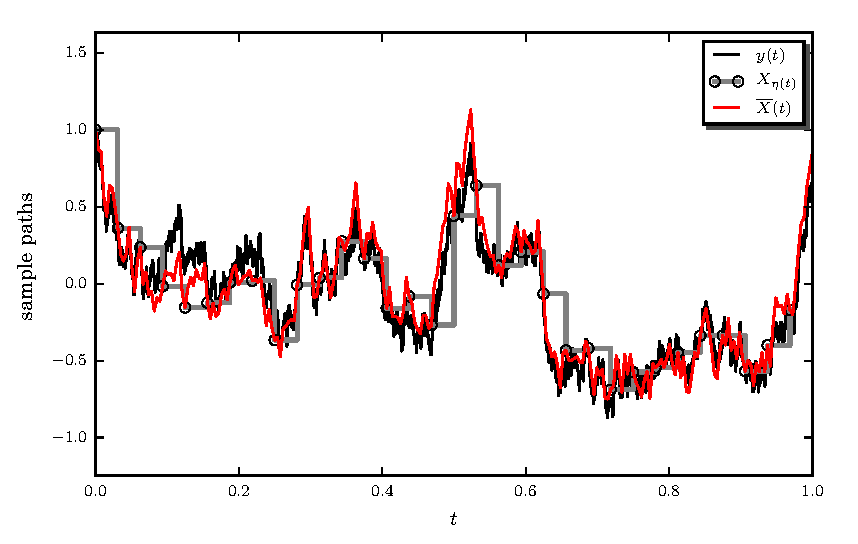
\includegraphics{papers/paperB/sections/ContinuousExtPy/ContinuousExtension.eps}
	\caption{
		The red line represents the continuous extension of the EM scheme. The continuous gray line is the 
		$Y_{\eta(t)}$ 
		process defined in \eqref{eqn:EulerMaruyama}.
	}
	\label{fig:ContinuousExtension}
\end{figure}
Using the continuous extension \eqref{eqn:EMContinuousExtension}
and the uniform mean square norm, the authors work with a stronger version of the ms-error%, which is given by 
$$
	\EX{\sup_{0\leq t \leq t}|y(t)-\overline{Y}(t)|^2}.
$$
%
Then, in  order to prove strong convergence of the EM method, the authors require the following assumptions.
\begin{assumption}\label{ass:HighamAssumption}
	For each $R>0$ there is a positive constant $C_R$, depending only on $R$, such that
	\begin{equation}\label{ass:LipschitzCondition}
		|f(x)-f(y)|^2 \vee |g(x)-g(y)|^2 \leq C_R|x-y|^2,
		\quad
		\forall x,y\in \R^d 
		\text{ with } |x|\vee |y|\leq R.
	\end{equation}
	And for some $p>2$, there is a constant $A$ such that
	\begin{equation}
		\EX{\sup_{0\leq t\leq T}|\overline{Y}(t)|^p}
		\vee
		\EX{\sup_{0\leq t\leq T}|y(t)|^p} \leq A.
	\end{equation}
\end{assumption}
In \cite{Higham2002b}, the authors prove that the \Cref{ass:HighamAssumption} is sufficient to ensure strong 
convergence for the EM scheme, namely 
\begin{thm}[
	{\cite[Thm 2.2]{Higham2002b}}
	]\label{thm:HighamMaoStuart}
	Under \Cref{ass:HighamAssumption}, the EM scheme \eqref{eqn:EulerMaruyama} with continuous extension
	\eqref{eqn:EMContinuousExtension}
	%\eqref{eqn:EMIntegralContinuousExtension} 
	satisfies
	\begin{equation}
		\lim_{h\to 0}
		\EX{\sup_{0\leq t\leq T}|\overline{Y}(t)-y(t)|^2}=0.
	\end{equation}
\end{thm}
	
	Applying this result, the authors prove the strong convergence of an implicit split-step variant of the EM, the
SSEM method. 
Their technique consist in proving each assertion of the following steps.
\begin{enumerate}[\bf{Step} 1:]
	\item
		\label{stp:EMCorrespondence}
		The SSEM for SDE \eqref{eqn:SDE1} is equivalent to the EM for the following conveniently SDE
		\begin{equation}\label{eqn:PerturbedHighamSDE}
			dy_h(t)= f_h(y_h(t))dt +g_h(y_h(t))dW(t).
		\end{equation}
	\item\label{stp:PerturbedSolution}
			The solution of the modified SDE \eqref{eqn:PerturbedHighamSDE} has bounded moments and it is 
			"close" to  $y$ the sense of the uniform mean square norm 
			$
				\EX{\sup_{0\leq t\leq T}|\cdot|^2}
			$.
	\item
	\label{stp:MethodBoundedMoments}
		Show that the SSEM method for the SDE \eqref{eqn:SDE1} has bounded moments.
	\item
		There is a continuous extension of the SSEM, $\overline{Z}(t)$, with bounded moments.
	\item
		Use the above steps and \Cref{thm:HighamMaoStuart} to conclude that
		\begin{equation}
			\lim_{h\to 0}
			\left\{
				\EX{\sup_{0\leq t\leq T}|y_h(t)-y(t)|^2}
			+
			\EX{\sup_{0\leq t\leq T}|\overline{Z}(t) -y_h(t)|^2}
			\right\}=0.
		\end{equation}
\end{enumerate}
In Chapter 4, we will use this technique.
% We will 
%use the same technique as these authors, that is, we will show that:
%\begin{inparaenum}[(a)]
%	\item
%		the underlying method corresponds to the EM for a perturbed SDE and
%	\item
%		all moments of the approximation are bounded.
%\end{inparaenum}
%
	Moreover, if we are interested in simulating the solution of the SDE \eqref{eqn:SDE} for large periods of time, 
	we need to use stable methods. We can interpret the stability of a numerical scheme, in some sense, as its
	capacity to preserve the  dynamical structure of the solution in that sense. Here we recall the topics that we will 
	work in the next chapter.
\subsection{Numerical Stability}
	With a numerical stability  one obtain  the step sizes for which a method reproduces  behavior of the solution 
	for a SDE. Therefore, it is important to know some qualitative  information  about the  solution, for example: if 
	all solution paths tend to a fixed point, or  if stay on a bounded set or reach an absorbent process.
	Usually the first step in this direction is a linear stability analysis. This study mimics the deterministic 
	context, which is based in the following steps:
	\begin{enumerate}[\bfseries{Step} 1:]
		\item 
			Expand in Taylor series around a fixed point the right hand side of a nonlinear ordinary differential 
			equation $x'(t) = f(t,x)$.
		\item
			Take a linear system with the Jacobian matrix of $f$ evaluated at the equilibrium
			$x'(t) = Ax(t)$.
		\item
			Diagonalize to decouples the linear system and study equations of the form
			$x'(t) = \lambda x(t), \lambda \in \C$.
	\end{enumerate}
	If all eigenvalues of $A$ are different from zero, then the  theorem of Hartman (see \cite{Hartman1960}) justifies 
	the use of this last equation  to study the behavior around a sufficient small neighborhood. So, one 
	seek conditions to assure that the numerical methods preserves the dynamics of underlying test. 
		
		In stochastic numerics, the linearization procedure is analogous  but here the linear SDE with multiplicative 
	noise is the benchmark test. The advantage of this linear SDE is that has the same unique fixed point as its 
	deterministic analogous, the origin \cite[]{Higham2000} .  Another benchmark equation is the linear SDE with 
	additive noise. However, for these model the concepts of numerical stability were unclear. The first works with 
	this test\cite{Hernandez1992,Milstein2004,Artemiev1997}, differs about the meaning of fixed point and stability. 
	Recently, the works of \citeauthor*{CruzCancino2010} \cite{CruzCancino2010} and \citeauthor*{Buckwar2011a} 
	\cite{Buckwar2011a} analyze the additive linear SDE using the theory of random dynamical systems, which in our 
	opinion clarifies this issue.
	
		Naturally the nonlinear case, is even more complex. Although  Lyapunov theory is the usual approach in 
	applications \cite{Khasminskii2011}, a more general novel approach based on the theory of random dynamical 
	systems \cite{Arnold1998} is a current topic of interest. In the following we provide this notions. 
		
\section*{Linear Stability}
	\subsection*{Multiplicative noise}
		Consider the scalar linear SDE
		\begin{equation}\label{eqn:SDEMultiplicativeNoise}
			dy(t)=\lambda y(t)dt+\xi y(t) dW(t) , \quad X_0=x_0,  \quad \lambda,\xi \in \C.
		\end{equation}
		The solutions of this SDE have the following property
		\begin{equation}\label{eqn:LinearMSEquivalence}
			\lim_{t\to\infty} \EX{|y(t)|^2} = 0 \Leftrightarrow \Re(\lambda) +\frac{1}{2} |\xi|^ 2 <0.
		\end{equation}
		A solution that satisfies  the previous limit  is a \emph{mean-square stable} solution. 
		Note that for $\xi = 0$ we have, $\Re(\lambda)<0$, which is the stability condition  for the deterministic case.
			
			Applying the EM method \eqref{eqn:EulerMaruyama} to \eqref{eqn:SDEMultiplicativeNoise}, we obtain
		\begin{equation}\label{eqn:MS-EMRecurrence}
			Y_{k+1} = \left(1 + h\lambda + \sqrt{h}\xi V_k\right)Y_k,
		\end{equation}
		where each $V_k$ is an independent $\calN(0,1)$ random variable. 
		In order to study the stability properties of the EM scheme, we must study
		the long time behavior of random variables of the form \eqref{eqn:MS-EMRecurrence}.
		Analogously, we will say that sequence \eqref{eqn:MS-EMRecurrence} is mean-square stable if 
		$
			\lim_{k \to  \infty}
				\EX{|Y_k|^2} = 0.
		$
		Note that the EM scheme depends upon the problem parameters $\lambda$ and  $\xi$, and the method
		parameter $h$. Then for a particular choice of parameters, we will say that the EM scheme is mean-square stable 
		if it produces a mean-square stable sequence. 
		Our interest lies in finding the parameter values for which the EM method is stable, and comparing results
		with the region $\Re(\lambda) + \frac{1}{2}|\xi|^2 < 0$ in \eqref{eqn:LinearMSEquivalence}
		for the underlying SDE (see \Cref{fig:StabilityPlotsMultiplicativeEM}). There is the following 
		result. 
		\begin{thm}
			Consider the EM method for the linear scalar SDE \eqref{eqn:SDEMultiplicativeNoise}. If the parameters 
			$\lambda$, $\xi$, and the step size $h$ satisfies
			$$
				\Re(\lambda) + \frac{1}{2}
				\left( |\xi|^2 + h|\lambda|^2\right) <0.
			$$
			Then the EM solution is \emph{mean square stable}.
		\end{thm}
		
		\begin{figure}[htb]
			\centering
			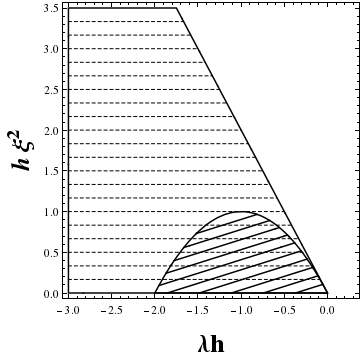
\includegraphics[scale=0.6]{Preliminaries/figures/StabilityPlotsMultiplicativeEM.png}
			\caption{Mean square regions of stability. The horizontal lines represents the stability region of
				SDE \eqref{eqn:SDEMultiplicativeNoise} and diagonal lines for the EM solution.
			}
			\label{fig:StabilityPlotsMultiplicativeEM}
		\end{figure}
			
	\subsection*{Additive noise}
	Here we study the additive linear SDE: 
	\begin{equation}\label{eqn:SDELinearAdditive}
		dy(t)=\lambda y(t)dt+ \xi  dW(t) , \qquad y_0=y_(t_0), \qquad \lambda, \xi \in \R.		
	\end{equation}
	where $\lambda$, $\xi \in \mathbb{C}$ and $X_{t_0}$ is the initial value of the process
	at time $t_0$. Equation \eqref{eqn:SDELinearAdditive}  has  the following  exact solution:
	\begin{equation}\label{eqn:IntroOUProcess}
	y(t)=\exp(\lambda (t-t_0)) y(t_0)+\xi 
	\exp(\lambda t)\int\limits_{t_0}^{t}\exp(-\lambda s)dW(s), 
	\qquad t\geq t_0.
	\end{equation}
	The stochastic process $y(t)$ defined in \eqref{eqn:IntroOUProcess} is known as 
	the {\it Ornstein-Uhlenbeck}'s (OU)  process. According to \cite{Hernandez1992},
	the OU process  is {\it asymptotically mean stable} if
	$ \lim_{t\to\infty}\m{y(t)}=0$ and is
	{\it  asymptotically  mean square stable} if
	$\displaystyle \lim_{t\to\infty}\ms{y(t)}=-\xi/2Re(\lambda)$. Both 
	limits are verified if $\lambda<0$. 
	Analogous stability properties are given for 
	stochastic  difference equations with additive noise \cite{SaiotoPreprint}. 
	Now, if we consider $\lambda<0$ then the OU solution \eqref{eqn:OUProcess} does 
	not convergence as $t$ tends to infinity but has the following pullback limit:
	\begin{equation}\label{eq4}
		\lim_{t_0\to-\infty} y(t)=\widehat{O}_t:=
		\exp(\lambda t)\int\limits_{-\infty}^{t}\exp(-\lambda s)dW(s), 
	\end{equation}
	$W(t)$  is now defined for all $t\in\mathbb{R}$, see
	\cite{Arnold1998, kloeden1999towards}. Furthermore, the process \eqref{eq4} is a
	stationary solution  of the additive linear SDE which attracts all other solutions in
	forward time and path-wise sense. Moreover, it is a finite process for all $t\geq
	T_{D(\omega)}$ ($\omega\in \Omega$) for  appropriate families $D(\omega)$ of bounded
	sets of initial conditions, see \cite{Robinson2002}. Therefore, 
	we can evaluate the numerical stability of a given stochastic method by examine if 
	this scheme reproduce the pullback asymptotic behavior.
	For example, the explicit EM scheme for \eqref{eqn:SDELinearAdditive}
	$$
		Y_{k+1} = (1+\lambda h) Y_n + \xi \Delta W_n,	
	$$
	given a initial value $Y_{k_0}$, has the form
	$$
		Y_{k+1} = (1+\lambda h)^{k-k_0} Y_{k_0}
			+\xi \sum_{j=k_0}^{k-1} (1+\lambda h)^{k-1-j} \Delta W_j.
	$$
	So, the path-wise pullback limit (taking $k_0 \to \infty$  with $k$ held fixed and $Y_{k_0} = Y_0$ for
	all $Y_{k_0}$ and constant time step $h$) exists, provided that $0 <h< 2/(- \lambda)$, $\lambda <0$, and is given
	by
	$$
		\widehat{O}_k^{(h)} := 
			\xi \sum_{j= -\infty}^k
				(1+\lambda h)^{1-k-j} \Delta W_j,
	$$
	for more details see the work of
	\citet*{Buckwar2011a}.
	
\section*{Non-Linear Stability}	
	Now we discuss the nonlinear case for multiplicative and additive noise. 
	\subsection*{Multiplicative Noise}
	We start with a notion of stability	which emulates the continuity respect to initial conditions of deterministic 
	ODEs.
	\begin{dfn}[\citeauthor{Baker2000a} {\cite{Baker2000a}}]\label{dfn:SNMS}
		Let $Y_n$ and $\widehat{Y}_n$ two different numerical recurrences  with
		corresponding initial process  $Y_0$ and $\widehat{Y}_0$. We shall say that a
		discrete time, $Y$ is \emph{numerically zero-stable in quadratic mean-square sense} if given
		$\epsilon >0$, there  are positive constants $h_0$ and $\delta=\delta(\epsilon,h_0)$
		such that for all $h\in(0,h_0)$ and positive integers $n \leq T/h$ whenever
		$\ms{Y_0-\widehat{Y}_0}<\delta$ then
		\begin {eqnarray}\label{eqn:SNMS}
		\rho_n :=
		\ms{Y_n-\widehat{Y}_{n}}<\epsilon .
	\end{eqnarray}
	If the method is stable and $\rho_n \to 0$ when $n\to \infty$, then the method is
	\emph{asymptotically zero-stable in the quadratic mean-square sense}.
\end{dfn}
Also, in \cite{Baker2000a} provides a result to characterizes this type of stability. Here we
enunciated it for the EM.
\begin{thm}[{\cite[Thm. 4 ]{Baker2000a}}]
	Let $C_1$, $C_2$ and $C_3$ generic positive constants which not depends on $h$ and $V$ a
	$\calN(0,1)$ random variable. 
	If the coefficients of  SDE \eqref{eqn:SDE} satisfies the estimates
	\begin{align*}
		\left|\EX{
			f(x) h +  g(x)\sqrt{h}V -
			\left(
				f(x') h + g(x')\sqrt{h}V
			\right)}	
		\right| 
		&\leq C_1h \left(|x - x'| \right), \\
		\EX{\left|
				hf(x)+g(x)\sqrt{h}V -
				\left(
				 f(x') h + g(x')\sqrt{h}V
				\right)	
			\right|^2}
			&\leq C_2 h \left(|x - x'| \right),
	\end{align*}
	then the EM method \eqref{eqn:EulerMaruyama} for \eqref{eqn:SDE} is zero-stable in the quadratic mean-square sense.
\end{thm}
%%%%%%%%%%%%%%%%%%%%%%%%%%%%%%%%%%%%%%%%%%%%%%%%%%%%%%%%%%%%%%%%%%%%%%%%%%%%%%%%%%%%%%%%%%
\subsection*{Additive noise}
		Nonlinear differential equations have more complex  dynamics than the linear case and
	the same  occurs for the finite difference equations. So,  \citeauthor*{Caraballo2006} in
	\cite{Caraballo2006}  extend the nonlinear stability theory of the deterministic
	numerical  analysis given in \cite{kloeden1999towards} to the stochastic
	case. They propose and justify the use of the following SDE as a test equation with additive noise:
	\begin{equation}\label{eqn:SemilinearSDE}
		dy(t)=\left(Ay(ts)+f(y(t))\right)dt+\xi dW(t),
	\end{equation}
	where $A$ is a $d \times d$ stiff matrix and function $f : \R^d \to \R^d $ is a nonlinear and non-stiff function 
	that satisfies, a
	{\it contractive one-sided Lipschitz} condition with constant
	$L_1>0$
	\begin{equation}\label{cl}
		\langle
			u - v,f(u)-f(v)
		\rangle\leq
		-L_1|u-v|^2\qquad \forall u,v\in \mathbb{R}^d.
	\end{equation}
Also the authors give sufficient conditions to assure an asymptotically stable stochastic stationary solution
of \eqref{eqn:SemilinearSDE}. In this context they establish the following result for the stability of $\theta$-EM 
scheme.
\begin{thm}[{\cite[Thm. 3.1]{Buckwar2011a}}]
	Suppose that the drift coefficient satisfies a contractive one-sided Lipschitz condition, and that the vector field 
	f satisfies a globally Lipschitz condition . Then the $\theta$-EM scheme has a unique stochastic stationary 
	solution 
	which is pathwise asymptotically stable for all step sizes $h> 0$
	if
	$$
		(1-\theta) (|A|+L) <-\theta (\mu[A] - L_1),
		\qquad
		\mu[A] = \lim_{\delta \to 0^+} \frac{(|Id + \delta A|)}{\delta},
	$$
	where $L$ refers to the Lipschitz condition and $L_1$  the to contractive one-sided Lipschitz condition.
\end{thm}












The following chapter shows adaptations of these results for the construction of a new method, the Steklov method.


	\chapter{Steklov method for scalar SDEs with Globally Lipschitz coefficients}
		\label{ch:Chapter3}
			\label{paper:paperA}
	%\section{Introduction} \label{sec1}
		\import{papers/paperA/sections/}{introduction.tex}
	\section{Steklov Method}\label{sec:SteklovMethod}
		\import{papers/paperA/sections/}{SteklovMethod.tex}
	\section{Strong consistency and convergence}\label{sec:StrongConsistencyAndConvergence}
		\import{papers/paperA/sections/}{StrongConsistencyConvergence.tex}
	\section{Linear Stability}\label{sec:LinearStability}
		\import{papers/paperA/sections/}{LinearStability.tex}
	\section{Nonlinear Stability} \label{sec:NonlinearStability}
		\import{papers/paperA/sections/}{NonLinearStability.tex}
	\section{Numerical Results}\label{sec:NumericalResults}
		\import{papers/paperA/sections/}{NumericalResults.tex}
	\chapter{Steklov Method for SDEs with Non-Globally Lipschitz Continuous Drift}
		\label{ch:Chapter4}
		\label{paper:paperB}
	\section{Introduction}
		%	Applications of Monte Carlo type simulations \cite{Glasserman2004,Giles2008} as  Brownian Dynamics \cite{Cruz2012}
%require  fast numerical methods with low computational cost --- excluding the use of 
%implicit schemes in the majority of cases.
%The EM method is the most popular in such  
%simulations due to its simple algebraic structure, cheap computational cost and acceptable convergence rate 
%under global Lipschitz conditions. 
%However, if the drift or diffusion coefficient of stochastic 
%differential equation  is super-linear, then the EM approximation 
%diverges  in the mean square sense \cite{Hutzenthaler2009, Hutzenthaler2012b}. 
%In most applications, the coefficients of the stochastic  models in finances, biology or physics 
%have locally Lipschitz coefficients with super-linear growth. 
%Therefore, recent research has been focused on modifying the EM method to obtain strong convergence  under these 
%conditions keeping its simple structure and  its low computational cost. In the last years, 
%several methods have been developed in this direction:  the family of  Tamed schemes
%\cite{Hutzenthaler2012a, Wang2011, Zong2014,Hutzenthaler2015,Sabanis2015}, 
%a special type of balanced method \cite{Tretyakov2013},  the stopped scheme \cite{Liu2013a} and 
%a truncated Euler method  \cite{Mao2015}.
%In these works, the strong convergence of the proposed method
%is proved using the theory developed by Higham, Stuart and 
%Mao in \cite{Higham2002b} or by means of  the new approach given by  Hutzenthaler and Jentzen in 
%\cite{Hutzenthaler2015}.
%Both techniques obtain the property of  strong convergence by proving boundedness moments of the numerical and 
%analytical solution of the underlying SDE. In spite of the recent work in this subject,  it is still necessary
%to get more accurate numerical methods for SDE under super-linear growth and 
%non-globally Lipschitz coefficients.

	In this chapter, we develop an explicit method based on a linear version  of the Steklov method proposed 
in  \Cref{ch:Chapter3}. We consider the vector It\^o stochastic differential equation
\begin{equation}\label{eqn:SDE1}
	dy(t)
	 =f(y(t))dt + g(y(t))dW(t), \quad 0\leq t\leq T,
	\quad y(0)=y_0,
\end{equation}
where $(f^{(1)},\dots, f^{(d)}):\R^d \to \R^d$ is one sided Lipschitz and 
$g = (g^{(j,i)})_{j\in \{1,\dots,d\}, i\in\{1,\dots, m\}}:\R^d \to \R^{d\times m}$ is global Lipschitz. 
Also we assume 
that  each component function $f^{(j)}$  can be written of the form
\begin{equation}\label{eqn:AlternativeConstruction}
	f^{(j)}(x) = a_j(x) x^{(j)} + b_j (x^{(-j)}), 
\end{equation}
where $a_j$ and	$b_{j}$ are two scalar 	functions in  $\R^d$ 
and $x^{(-j)} = \left( x^{(1)},\dots,x^{(j-1)},x^{(j+1)},\dots x^{(d)}\right)$.%
	\section{General Settings}
		
Throughout this paper, 
we work with a standard setup, that is,  $y(t)\in \R^d$ for each 
$t$ and  $W(t)$ is a
$m$-dimensional standard Brownian motion on a filtered and complete probability space
$	(
		\Omega ,\calF,(\calF_t)_{t\in[0,T]},\prob{}
	)$,
with the filtration
$(\mathcal{F}_t)_{t\in[0,T]}$  generated by the Brownian process.  Moreover,
we denote  the norm of a vector $y\in \R^d$ and the Frobenious norm 
of a matrix $G\in \R^{d\times m}$  by $|y|$ and $|G|$ respectively. The usual scalar product of two vectors 
$x,y\in \R^d$ is denoted by $\innerprod{x}{y}$.  The complement of a set $E$ is denoted by $E^c$ and 
the indicator function  of the set $E$ is denoted by $\1{E}$. 
In the following, we recall some classical results  about the moment boundedness, existence 
and uniqueness of the solution of the stochastic differential system \eqref{eqn:SDE1}, 
see \cite{Higham2002b,Mao2013,Mao2007}. We  also state some theorems about the strong 
convergence of the Euler-Maruyama method given by Higham et al. in \cite{Higham2002b} which will be useful 
 to prove the strong convergence of the Linear Steklov method. 
 
Let us start by assuming the following:


	
\begin{hypothesis}\label[hypothesis]{ass:OSLC}
	The coefficients of SDE \eqref{eqn:SDE1} satisfy the conditions:
	\begin{enumerate}[({H}-1)]
		\item \label{ass:C1Functions}
		The functions $f,g$ are in the class $C^{1}(\R^d)$.
		\item
		\textbf{Local, global Lipschitz condition}. For each integer $n$, there is a positive
		constant $L_{f}=L_{f}(n)$ such that
		$$
		|f(u)-f(v)|^2 %\vee |g(x)-g(y)|^2
		\leq L_{f}|u-v|^2 \qquad \forall u,v \in \R^d, \qquad |u|\vee|v|\leq n,
		$$
		and there is a positive constant $L_g$ such that
		$$
		|g(u)-g(v)|^2 \leq L_{g}|u-v|^2,
		\qquad  \forall u,v \in \R^d.
		$$ 
		\item\label{ass:MonotoneCondition}
		\textbf{Monotone condition.} There exist two positive constants $\alpha$ and $\beta$
		such that
		\begin{equation}\label{eqn:MonotoneCondition}
		\innerprod{u}{f(u)} +\frac{1}{2}|g(u)|^2
		\leq \alpha +\beta |u|^2, \qquad \forall u \in \R^d.
		\end{equation}
	\end{enumerate}
\end{hypothesis}


Under \Cref{ass:OSLC} we can assure  existence and uniqueness 
of the solution of continuous system \eqref{eqn:SDE1}. Next we state  the bounds on the moments
 of the  solution of \eqref{eqn:SDE1}.
%
 \begin{thm}
 	Assume \Cref{ass:OSLC}  then for all $y(0)=y_0\in \mathbb{R}^d$   there exists a 
 	unique global solution $\{y(t)\}_{t\geq 0}$ to SDE \eqref{eqn:SDE1}. Moreover, the solution has the 
 	following properties for any $T>0$,
 	\begin{equation*}
 		\ms{y(T)}< 
 		\left(
 			|y_0|^2 +2\alpha T 
 		\right)e^{2\beta T},
 	\end{equation*}
 	and
 	\begin{equation*}
 	\Prob{\tau_n\leq T}
 	\leq \frac{
 		\left(
 		|y_0|^2 +2\alpha T 
 		\right)
 		e^{2\beta T}
 	}{n},
 	\end{equation*}
 	where $n$ is any positive integer and 
 	%\begin{equation*}
 	$\tau_n := \inf \{ t\geq 0 : |y(t)|>n\}$.
 	%\end{equation*}
 \end{thm}
% %
\begin{thm}
	\label{thm:MaoCoercive}
	Let $p\geq 2$ and $x_0\in L^p(\Omega, \mathbb{R}^d)$. Assume that there exits a constant $C>0$
	such that for all $(x,t)\in \mathbb{R}^d\times [t_0,T]$,
	\begin{equation*}
	\innerprod{x}{f(x,t)}+\frac{p-1}{2}|g(x,t)|^2 \leq C(1+|x|^2).
	\end{equation*}
	Then
	\begin{eqnarray*}
	\EX{\sup_{0\leq t \leq T}|y(t)|^p}&\leq& C \left(1+\mep{y_0}\right), \nonumber\\
	\m|y(t)|^p
	&\leq&
	2^{\frac{p-2}{2}}
	\left(
	1 + \m|y_0|^p
	\right)e^{Cpt}, \qquad \forall t\in[0,T].
	\end{eqnarray*}
\end{thm}
\begin{hypothesis}\label{ass:MomentBounds}
	The SDE \eqref{eqn:SDE1} the EM solution \eqref{eqn:EulerMaruyama} and its continuous extension 
	\eqref{eqn:EMContinuousExtension} satisfies
	\begin{equation*}
		\EX{
			\sup_{0\leq t\leq T}
			|y(t)|^p	
		}< \infty, \quad
	\EX{
		\sup_{0\leq k \leq N}
			|Y_k|^p	
	}< \infty, \quad
	\EX{
		\sup_{0\leq t\leq T}
		|\overline{Y}(t)|^p	
	} < \infty, \qquad \forall p\geq 1.
	\end{equation*}
\end{hypothesis}

%********************************************************************************************
%              Section 3
%********************************************************************************************


		%
\begin{thm}[{
		%\citeauthor{Mao2013}
	 \cite[Thm. 2.2]{Mao2013}}]
	Let \Cref{ass:OSLC} holds. Then for all $y(0)=y_0\in \mathbb{R}^d$ given, there exist a 
	unique global solution $\{y(t)\}_{t\geq 0}$ to SDE\eqref{eqn:SDE1}. Moreover, the solution has the 
	following properties for any $T>0$,
	\begin{equation*}
		\ms{y(T)}< 
		\left(
			|y_0|^2 +2\alpha T 
		\right)\exp(2\beta T),
	\end{equation*}
	and
	\begin{equation*}
	\Prob{\tau_n\leq T}
	\leq \frac{
		\left(
		|y_0|^2 +2\alpha T 
		\right)
		\exp(2\beta T)
	}{n},
	\end{equation*}
	where $n$ is any positive integer and 
	%\begin{equation*}
	$\tau_n := \inf \{ t\geq 0 : |y(t)|>n\}$.
	%\end{equation*}
\end{thm}
%
\begin{thm}[
		%\citeauthor{Mao2007} 
		{\cite[Thm. 2.4.1]{Mao2007}}
	]
	\label{thm:MaoCoercive}
	Let $p\geq 2$ and $x_0\in L^p(\Omega, \mathbb{R}^d)$. Assume that there exits a constant $C>0$
	such that for all $(x,t)\in \mathbb{R}^d\times [t_0,T]$,
	\begin{equation*}
	\innerprod{x}{f(x,t)}+\frac{p-1}{2}|g(x,t)|^2 \leq C(1+|x|^2).
	\end{equation*}
	Then
	\begin{equation*}
	\m|y(t)|^p
	\leq
	2^{\frac{p-2}{2}}
	\left(
	1 + \m|y_0|^p
	\right)\exp({Cpt}) \quad \text{ for all } t\in[0,T].
	\end{equation*}
\end{thm}
%
\begin{lem}[
	{
		%\citeauthor{Higham2002b}
		\cite[Lem 3.2]{Higham2002b}}
	]
	\label{lem:MomentBound}
	Under \Cref{ass:OSLC}, for each $p\geq 2$, there is a $C=C(p,T)$ such that
	\begin{equation*}
	\EX{\sup_{0\leq t \leq T}|y(t)|^p}\leq C \left(1+\mep{y_0}\right).
	\end{equation*}
\end{lem}
%
	\section{Construction of the LS Method}
		%
	For simplicity, we begin the construction of the Linear Steklov method (\SM) considering the scalar case of SDE 
\eqref{eqn:SDE1}, that is, when $d=m=1$, also, to shorten notation we use $a,b$ instead $a_j,b_j$. 
Tough this ideas, we will generalize to higher dimensions.
Let $0=t_0 < t_1< \cdots < t_N=T$ a partition of the interval $[0,T]$ with constant step-size $h=T/N$ and such that
$t_k=kh$ for $k=0,\ldots, N$. The main idea of the  \SM approximation  consists in 
estimating the drift coefficient of \eqref{eqn:SDE1}  by
\begin{equation}
	f(y(t)) \approx 
		\varphi_{f}(y(t_{\eta_{+}(t)})) =
		\left(
			\frac{1}{y(t_{\eta_+(t)})-y(t_{\eta (t)})}
			\bigint \limits
_				{y(t_{\eta(t)})}^{y(t_{\eta_+(t)})}
					\frac{du}
						{
							a(y(t_{\eta(t)}))u
							+b
						}
	\right)^{-1}, \qquad t\in [0,T],
\end{equation}
where
\begin{align*}
	\eta(t) &:=
	k\text{  for } t\in [t_k, t_{k+1}), \quad k\geq 0,\\
	\eta_{+}(t) &:= 
	k+1  \text{ for } t\in [t_k, t_{k+1}), \quad k\geq 0.
\end{align*}
So we define the \SM method for the scalar version of the SDE \eqref{eqn:SDE1} using a split-step formulation as follows
\begin{align}
	Y_k^{\star} &= Y_k + h \varphi_f(Y^{\star}_k), \label{eqn:SSLSM1}\\
	Y_{k+1}	&= Y_k^{\star} + g(Y_k^{\star})\Delta W_k \label{eqn:SSLSM2},
\end{align}
with $Y_0=y_0$ and  $\varphi_{f}\left(Y_k^{\star}\right)$ defined by 
\begin{equation}
	\varphi_{f}\left(Y_k^{\star}\right)
	=
		\left(
			\frac{1}{Y_{k}^{\star}-Y_{k}}
			\int 
			%\limits
			_{Y_{k}}^{Y_{k}^{\star}}
				\frac{du}
				{
					a(Y_k)u
					+b
				}
	\right)^{-1}
\end{equation}
This scheme combines a split-step technique with a linear version of an exact deterministic 
method see \cite{Diaz-Infante2015,Matus2005}. 
In detail, first we compute the discrete value $Y^{\star}_k$ using the Linear Steklov approximation \eqref{eqn:SSLSM1},
and next, $Y_{k+1}$ is obtained by adding the stochastic increment $g(Y_k^\star)\Delta W_k$.

	To higher dimensions, we adapt the same split step scheme \crefrange{eqn:SSLSM1}{eqn:SSLSM2} as follows. 
For each component equation $j\in\{1, \ldots,  d\}$, on the iteration $k\in\{1, \ldots,  N\}$ take
\begin{align}
	a_{j,k} &=
	a_j
	\left(
		Y^{(1)}_{k},
		\ldots, Y^{(d)}_{k}
	\right),
	&
	b_{j,k} =
	b_{j}
	\left(
			Y^{(-j)}_k
	\right).
\end{align}
So, define  
$
	\varphi_{f}(Y_k^{\star})=
		\left(
			\varphi_{f^{(1)}}(Y_k^{\star}),
			\ldots,
			\varphi_{f^{(d)}}(Y_k^{\star})
		\right)
$
by
\begin{equation}
	\varphi_{f^{(j)}}\left(Y_k^{\star}\right)
		=
		\left(
			\frac{1}{Y_{k}^{\star(j)}-Y_{k}^{(j)}}
			\int 
			%\limits
				_{Y_{k}^{(j)}}^{Y_{k}^{\star(j)}}
				\frac{du}
				{
					a_{j,k} u
					+b_{j,k}
				}
		\right)^{-1}.
\end{equation}
%
	It is worth mentioning that even this formulation is semi implicit, we always can derive a explicit version. 
The next result deals with this issue. To simplify notation, we define  $A^{(1)}= A^{(1)}(h,u)$,  $A^{(2)}=A^{(2)}(h,u)$  and $b=b(u)$ by 
\begin{align}\label{eqn:SolutionFunctions}	
	A^{(1)}&:=
		\begin{pmatrix}
			e^{ha_1(u)} & \multicolumn{2}{c}{\text{\kern0.5em\smash{\raisebox{-1ex}{\huge 0}}}} \\
			&\ddots\\
			\multicolumn{2}{c}{\text{\kern-0.5em\smash{\raisebox{0.95ex}{\huge 0}}}} 
			& e^{ha_d(u)}
		\end{pmatrix},
		\notag
		\\
		%	
	A^{(2)}&:=
	\begin{pmatrix}
		\left(
			\displaystyle
			\frac{e^{ha_1(u)} - 1}{a_1(u)}
		\right)\1{E_1^c}	& 
		\multicolumn{2}{c}{\text{\kern0.5em\smash{\raisebox{-1ex}{\huge 0}}}}\\
		 & \ddots&\\
		\multicolumn{2}{c}{\text{\kern0.5em\smash{\raisebox{-1ex}{\huge 0}}}}&
		\left(
			\displaystyle
			\frac{e^{ha_d(u)} - 1}{a_d(u)}
		\right)\1{E_d^c}% + h \1{E_i} 
	\end{pmatrix}
	+h
	\begin{pmatrix}
		\1{E_1} & \multicolumn{2}{c}{\text{\kern0.5em\smash{\raisebox{-1ex}{\huge 0}}}}\\
		&\ddots &\\
		\multicolumn{2}{c}{\text{\kern0.5em\smash{\raisebox{-1ex}{\huge 0}}}} &
		\1{E_d}
	\end{pmatrix},\\	
	E_j&:=\{x \in \R^d: a_j(x)=0\} , \qquad 
	b(u):= \left(
		b_1(u^{(-1)}), \dots , b_d(u^{(-d)})
	\right)^T.		
	\notag
\end{align}
	Also we will need the following results from \cite[Thm 2.1]{Lawlor2012}, \cite[Thm. 1]{FineAIandKass1966}.
The first theorem will help us  with the singularities of set $E_j$ in the case where all elements of this set
are limit points. 
\begin{thm}[Multivariate L'h\^{o}pital's Rule] \label{thm:Lawlor}
	Let $\mathcal{N}$ be a neighborhood in $\R^2$ containing a point $\mathbf{q}$ at which
	two differentiable functions $f:\mathcal{N}\to \R$ and $g:\mathcal{N}\to \R$ are zero.
	Set 
	$$
		C=\{x \in \mathcal{N}: f(x)=g(x)=0 \},
	$$
	and suppose that $C$ is a smooth curve through $\mathbf{q}$.
	
	Suppose	there exist a vector $\mathbf{v}$ not tangent to $C$ at $\mathbf{q}$
	such that the directional derivative $D_{\mathbf{v}}g$ of $g$ in the direction of $\mathbf{v}$ is never zero
	within $\mathcal{N}$. Also we assume that $\mathbf{q}$ is a limit point of $\mathcal{N}\setminus C$. Then
	\begin{equation*}
		\lim_{(x,y)\to \mathbf{q}}
		\frac{f(x,y)}{g(x,y)} =
		\lim_{
				\substack{
					(x,y)\to \mathbf{q}\\ 
					(x,y)\in \mathcal{N} \setminus C
				}
		}
		\frac{D_{\mathbf{v}} f }{D_{\mathbf{v}} g}
	\end{equation*}
	if the latter limit exist.
\end{thm}
For the second auxiliary we will need the following concepts.
\begin{dfn}[Directional derivative referred at a point]
	Let $u,\mathbf{q}\in \R^2$ and $\alpha$ the positive angle respect to the $x$-axis and the segment
	$\overline{u \mathbf{q}}$.	We denote by 
	\begin{align*}
		f_{\alpha}(u) &= 
			\cos(\alpha) 		
			\frac{\partial f}{\partial u^{(1)}}(u) + 
			\sin(\alpha)
			\frac{\partial f}{\partial u^{(2)}}(u) 
			= \frac{ \innerprod{q-u}{\nabla f(u)}}{|u-q|}			
	\end{align*}
	the \emph{directional derivative respect to the point $\mathbf{q}$ on $u$}.
\end{dfn}
\begin{dfn}[Star-like set]
	A set $S\subset \R^2$ is \emph{star-like} with respect a point $\mathbf{q}$, if for each point $s \in S$ the open 
	segment $\overline{s \mathbf{q}}$ is in $S$.
\end{dfn}
%
Whit this in mine, second theorem give us a way to analyze isolated singularities.
\begin{thm}\label{thm:Fine}
	Let $\mathbf{q}\in \R^2$ and let $f$,$g$ be functions whose domains include a set $S\subset \R^2$ which is 
	star-like 
	with  respect to the point $\mathbf{q}$. Suppose that on $S$ the functions are differentiable and that
	the directional derivative of $g$ with respect to $\mathbf{q}$ is never zero. With the understanding that all 
	limits are taken from within on $S$ at $\mathbf{q}$ and if
	\begin{enumerate}[(i)]
		\item 
			$f(\mathbf{q})=g(\mathbf{q})=0$,
		\item
			$
				\displaystyle
				\lim_{x \to \mathbf{q}}
				\frac{f_{\alpha}(x)}{g_{\alpha}(x)} = L,	
			$
	\end{enumerate}
	then
	$$
		\lim_{x \to \mathbf{q}}
		\frac{f(x)}{g(x)} = L.
	$$
\end{thm}
%
With this on mind, we additionally require the following. 
\begin{hypothesis}\label[hypothesis]{ass:ajBound} %\label{as:aiFunctions}
	For each component function $f^{(j)}:\R^d:\to \R$ %$j \in \{1, \dots, d \}$,
	with $j \in \{1,\dots, d\}$:
	\begin{enumerate}[({A}-1)]
		\item\label{ass:FunctionStructure}
		There are two locally Lipschitz functions of 
		class $C^1(\R^d)$ denoted by
		$a_j:\mathbb{R}^{d} \to \mathbb{R}$ and
		$b_{j}:\mathbb{R}^{d-1} \to \mathbb{R}$ such that 
		the $j$-component of the drift function can be rewritten 
		as in \eqref{eqn:AlternativeConstruction}.
		\item\label{a}
		There is a positive constant $L_a$ such that
		$$
		a_{j}(x) \leq L_a, \qquad\forall x\in \R^d.
		$$
		\item Each function $b_j(\cdot)$ satisfies the linear growth condition
		\begin{equation*}\label{eqn:bjLinearGrowthCondition}
		|b_j(x^{(-j)})|^2 \leq L_{b}(1+|x|^2) , \qquad \forall x\in \R^d.
		\end{equation*}
	\end{enumerate}
\end{hypothesis}

\begin{hypothesis} \label{ass:HypThmSingularities}
	The set $E_j:=\{x\in \R^{d}: a_j(x)=0\}$ satisfies either:
	\begin{enumerate}[(i)]
		\item
			All point $q \in E_j$ is a non isolated zero of $a_j$ and:
			\begin{itemize}
				\item the set 
					$$
						D:=\{u \in B_r(q): e^{ha_j(u)}-1=a_j(u)= 0\},
					$$ 
					is a smooth curve through $q$. 
				\item
					The canonical vector $e_j$ is not
					tangent to $D$.
				\item
					For each $q \in E_j$, there is an open ball with center
					on $q$ and radio $r$ $B_r(q)$, such that  
					and
					$$
						a_j\neq 0, \qquad
						\frac{\partial a_j(u)}{\partial u^{(j)}} \neq 0 ,\qquad 
						\forall u \in B_r(q)
						\setminus D.
					$$	
				%				
				%				\item
				%					The limit
				%					$$
				%						\lim_{
				%							\substack{
				%								u\to u^*\\ 
				%								u \in B_r(q) \setminus D
				%							}
				%						}
				%						\frac{e^{h a_j(h)} \frac{\partial a_j(u)}{\partial u^{(j)}}}{\frac{\partial a_j(u)}{\partial 
				%						u^{(j)}}}
				%					$$
				%					
			\end{itemize}	
		\item
			All point $q \in E_j$ is a isolated zero of $a_j$ and:
			\begin{itemize}
				\item
					For each $q\in E_j$,  $q$ is not a limit point of the set 
					$E_{\alpha}:=\{x \in \R^d: (a_j)_\alpha(x)=0\}$.
				\item
					For each $q \in E_j$ there is a star-like set respect to $q$ $E_q$, such that
					the directional derivative respect to $q$ satisfies
					$$
						 (a_j)_\alpha(x) \neq 0, \qquad \forall x\in E_q.
					$$
			\end{itemize}		
	\end{enumerate}	
\end{hypothesis}
%
By \Cref{ass:ajBound} there is a unique linear Steklov approximation and by \Cref{ass:HypThmSingularities}
we can apply  \Cref{thm:Lawlor} or \Cref{thm:Fine} to deals with possible singularities of the matrix function 
$A^{(2)}$ defined on \eqref{eqn:SolutionFunctions}. Under the previous  assumptions 
we will show that the explicit Linear  Steklov approximation \crefrange{eqn:SSLSM1}{eqn:SSLSM2}
exists, the function $\varphi_f$ is bounded by the drift function $f$ and also the 
coefficients $\varphi_f$  and $g$  satisfy a monotone condition. First, we will give the following lemma.
\begin{lem}\label{l1}
	Assume \Cref{ass:OSLC,ass:ajBound,ass:HypThmSingularities} hold. 
	The function $\Phi_j(x)=\Phi(h, a_j)(x)$ 
	defined by
	\begin{equation}\label{eqn:ExpBound}
		\Phi_j(x):=\frac{e^{ha_j(x)}-1}{ha_j(x)},
	\end{equation}
	is bounded  on $\R^d$ for each $j\in \{ 1,\dots, d\}$
	by a positive constant $L_{\Phi}$, which could depend on $h$.
\end{lem}
\begin{proof}    By \Cref{ass:OSLC}, the operator $\Phi$ is continuous
	on $E_j^c$, thus 
	\begin{equation}\label{e0}
	\lim_{h\to 0}
	\frac{e^{ha_j(x)}-1}{ha_j}=1,
	\end{equation}
	for each fixed $\in E_j^c$. If $x^*\in E_j$ and fixing any $h$, by \Cref{ass:HypThmSingularities}, 
	we obtain one of the following cases:
	\begin{equation}\label{eqn:ajSingularityCasei}
	\lim_{
		\substack{
			x \to x^*\\ 
			x\in E_j^c
		}
	}
	\Phi(h,a_j)(x) =
	%
	\lim_{
		\substack{
			x \to x^*\\ 
			x\in E_j^c
		}
	}	
	\frac{\frac{\partial a_j(x)}{\partial x^{(j)}} 
		h e^{h a_j(x)} 
	}{
	h\frac{\partial a_j(x)}{\partial x^{(j)}}
}=1,
\end{equation}	
or
\begin{equation}\label{eqn:ajSingularityCaseii}
\lim_{
	\substack{
		x \to x^*\\ 
		x\in E_j^c
	}
}
\Phi(h,a_j)(x) 
=
%
\lim_{
	\substack{
		x \to x^*\\ 
		x\in E_j^c
	}
}	
\frac{
	\left(
	e^{h a_j(x)} - 1
	\right)_{\alpha}
}{
\left(
h a_j(x)
\right)_{\alpha}
}	=	1, \qquad \alpha = 0,\pi, 2\pi,\dots
\end{equation}	
From \eqref{e0}, \eqref{eqn:ajSingularityCasei} and \eqref{eqn:ajSingularityCaseii} we can deduce that 	
\begin{equation}\label{eqn:PhiBound}
	\left|\frac{e^{ha_j(x)}-1}{ha_j(x)}
	\right|\leq\left|\frac{e^{hL_a}-1}{ha^*_j}
	\right|,
	\qquad \forall x \in \R^d,
\end{equation}
where $a^*_j:= \inf_{x\in E_j^c}\{|a_j(x)|\}$. So, for each $h$ fixed by inequality \eqref{eqn:PhiBound} we can 
deduce that there a positive constant $L_{\Phi}=L_{\Phi}(h)$ such that
$$
	|\Phi_j(x)|\leq L_{\Phi}, \qquad \forall j\in \{1,\dots, d\}.	
$$ 
Finally, if $a^*_j=0$, then we can
use an argument similar to \crefrange{eqn:ajSingularityCasei}{eqn:ajSingularityCaseii}.	
\end{proof}

Now we can state the following result.
\begin{lem}\label{lem:PhiFhProp}
	Let \Cref{ass:OSLC,ass:ajBound,ass:HypThmSingularities} holds, and $A^{(1)}$, $A^{(2)}$, $b$  
	defined by 
	\eqref{eqn:SolutionFunctions}. Then given $u\in\mathbb{R}^d$, the equation
	\begin{equation}\label{eqn:varphiEquation}
		v = u + h \varphi_f(v),
	\end{equation}
	has a unique solution 
	\begin{equation}\label{eqn:varphiEqnSolution}
		v = A^{(1)}(h,u)u +A^{(2)}(h,u) b(u)	.
	\end{equation}
%
	If we define the functions
	$F_h(\cdot)$, $\varphi_{f_h}(\cdot)$ and $g_h(\cdot)$ by
	\begin{equation}\label{eqn:FunctionshDefinition}
		F_h(u) = v,
%			\left(
%				u + \frac{b}{a(u)}
%			\right)\exp\left(ha(u)\right)
%				-\frac{b}{a(u)},
			\qquad 
			\varphi_{f_h}(u) =\varphi_{f}(F_h(u)),
			\qquad
			g_h(u) = g(F_h(u)),
	\end{equation}
	then $F_h(\cdot)$, $\varphi_{f_h}(\cdot)$, $g_h(\cdot)$ are local Lipschitz functions 
	and for all $u\in \mathbb{R}^d$ and each $h$ fixed, there is a positive constant $L_{\Phi}$ such that
	\begin{equation}\label{eqn:PhifhFbound}
		|\varphi_{f_h}(u)|\leq L_{\Phi} |f(u)|. 
	\end{equation} 
	Moreover, for each $h$ fixed,
	%$g_h$ is a locally Lipschitz function and 
	 there are positive constants $\alpha^*$ and  $\beta^*$ such that
	\begin{equation}\label{eqn:h-MonotoneCondition}
		\innerprod{\varphi_{f_h}(u)}{u} \vee |g_h(u)|^2 \leq \alpha^* + \beta^* |u|^2, 
		\qquad
		\forall u \in \R^d.
	\end{equation}
\end{lem}
%
\begin{proof}
Let us first prove that \eqref{eqn:varphiEqnSolution} is solution 
of equation \eqref{eqn:varphiEquation}.  Note that 
\begin{equation}\label{e1}
v^{(j)} = u^{(j)} + h \,\varphi_{f^{(j)}}(v),	
\end{equation}
for each $j\in \{1,\dots, d\}$ and using the linear Steklov function \eqref{ap}, 
we can derive that
\begin{equation}\label{r1}
v^{(j)}= e^{h a_j(u)} u^{(j)} + 
\left[
h\Phi_j(u)
\1{E_j^c}
+h \1{E_j}
\right]b_{j}(u^{(-j)}),
\end{equation}	
which is the $j$-component of the vector
$A^{(1)}u +A^{(2)} b(u)$. Now let us prove inequality \eqref{eqn:PhifhFbound}. Given that 
$v =\varphi_{f}(F_h(u))$, 
we can also rewrite \eqref{e1} as
$$
\varphi_{f_h}^{(j)}(u) = 
\frac{
	%				\displaystyle
	F_h^{(j)}(u)-u^{(j)}
}%
{%				
	\displaystyle
	\int_{u^{(j)}}^{F_h^{(j)}(u)}
	\frac{dz}{a_j(u)z + b_j(u^{(-j)})}
}.
$$
If $u\in E_j$ then $\varphi_{f_h}^{(j)}(u) = b_j(u^{(-j)}) = f^{j}(u)$,
so $L_{\Phi}\geq 1$ fulfills  \eqref{eqn:PhifhFbound}.
On the other hand, if $u\in E_j^c$ then
\begin{equation}\label{eqn:VarPhiEjc}
\varphi_{f_h}^{(j)}(u) =
\frac{
	(F_h^{(j)}(u)-u^{(j)}) a_j(u)
}
{
	\underbrace{
		\ln \left(
		a_j(u) F_h^{(j)}(u) + b_j(u^{(-j)})
		\right)
	}_{:=R_1}
	-
	\ln \left(
	a_j(u) u^{(j)} + b_j(u^{(-j)})
	\right)
}=\Phi_j(u)f^j(u),		
\end{equation}
where
\begin{equation}\label{eqn:Ter1Simplification}	
R_1=
\ln\left\{
a_j(u)\left[
e^{ha_j(u)}u^{(j)} +
h\Phi_j(u) b_j(u^{(-j)})	
\right]
+b_j\left(u^{(-j)}\right)
\right\} \notag \\
=h a_j(u) + \ln \left( f^{(j)}(u) \right).		
\end{equation}
By lemma \ref{l1}, inequality \eqref{eqn:PhifhFbound} is satisfied 
for all $u\in E_j \cup E_j^c$. 	As $g_h(x)=g\left(F_h(x) \right)$ 
by \Cref{ass:OSLC}, then
\begin{equation} \label{eqn:gLocalLipschitzArg} 
|g_h(u)-g_h(v)|^2 \leq
L_g|F_h(u)- F_h(v)|^2  \leq
2L_g \underbrace{
	|A^{(1)}u - A^{(1)}v|^2 
}_{:=R_2} +
2L_g \underbrace{
	|A^{(2)}b(u) - A^{(2)}b(v) |^2 
}_{:=R_3}.			
\end{equation}
Let us consider each term of the right hand of inequality \eqref{eqn:gLocalLipschitzArg}.
First, note that $A^{(1)}$ is a continuous differentiable function on all 
$\R^d$, so using the mean value theorem,
we have
\begin{equation}\label{eqn:BoundTer1gh}
R_2
\leq
L_{A^{(1)}}|u-v|^2, \quad u,v \in \R^d, \quad |u|\vee |v|\leq n,
\end{equation}
for a positive constant $L_{A^{(1)}} \geq \sup_{0\leq t \leq 1} 
|\partial A^{(1)}(h, u+t(v-u))|^2$. Meanwhile, 
\begin{eqnarray}
R_3 &=&\sum_{j=1}^d\Big[\1{E_j^c}(u) \Phi_j(u) b_j(u^{(-j)}) + h \1{E_j}(u) b_j(u^{(-j)}) 
-\1{E_j^c}(v) \Phi_j(v) b_j(u^{(-j)})\nonumber \\ &-& h \1{E_j}(v) b_j(v^{(-j)})
\Big]^2 
\leq
4\sum_{j=1}^d
\Big[
\left(	
\1{E_j^c}(u) L_{\Phi} b_j(u^{(-j)})  
\right)^2
+
\left(
h \1{E_j}(u) b_j(u^{(-j)})
\right)^2
\nonumber\\&+&
\left(
\1{E_j^c}(v) L_{\Phi} b_j(v^{(-j)})
\right)^2
+
\left(
h \1{E_j}(v) b_j(v^{(-j)}
\right)^2
\Big].
\label{eqn:BoundArgTer2}	
\end{eqnarray}	
Since  $b^2_j(\cdot)$ is a function of class $C^1(\R^d)$, there is a 
constant $L_b=L_b(n)$ such that
\begin{dmath}[label={eqn:Boundbju}]
	|b_j(u)|^2 \leq L_b 
	\condition{
		$\forall u \in \R^d$,
		\quad $|u| \vee |v| \leq n$,}		
\end{dmath}
for each $j \in \{1,\cdots, d\}$. Using this bound in  \eqref{eqn:BoundArgTer2}, we obtain
\begin{equation}\label{eqn:BoundL0Ter2gh}
R_3\leq
4 \sum_{j=1}^d
\left[
2 L_{\Phi} L_b +2h^2 L_b
\right] 
\leq L_0, \qquad
\forall u,v \in \R^d,
\quad |u|\vee|v| \leq n,
\end{equation}
where $L_0=8d L_b(n)(L_{\Phi}+h^2)$.
By inequalities \eqref{eqn:BoundTer1gh} and \eqref{eqn:BoundL0Ter2gh},  we get
\begin{equation}
|g_h(u) - g_h(v)|^2 \leq L_{g_h}(n) |u - v|^2, 
\qquad	\forall u,v \in \R^d,
\quad |u|\vee |v| \leq n,		
\end{equation}
where $L_{g_h}(n)\geq n^2+1+L_0+ L_{A^{(1)}}$. Then $g_h(\cdot)$ is a locally 
Lipschitz function. Furthermore, note that under some modifications
this argument can be used to prove that $F_h(\cdot)$ is also a locally Lipschitz 
function, which implies that $\varphi_{f_{h}}$ is a locally Lipschitz function.
Finally, we  will demonstrate inequality \eqref{eqn:h-MonotoneCondition}. 
By \Cref{ass:OSLC,ass:ajBound}, we have
\begin{equation*}\label{eqn:bDotProdBound}
	\innerprod{f(u)}{u}
	=
	\sum_{j=1}^d
	a_j(u) \left( u^{(j)} \right)^2
	+
	\sum_{j=1}^d
	b_j(u) u^{(j)}
	\leq \alpha +\beta |u|^2,
\end{equation*}
and
\begin{equation*}\label{eqn:bDotProdBound}
	\innerprod{b(u)}{u} \leq \alpha + (\beta + L_a)|u|^2.
\end{equation*}
Using these inequalities and \eqref{eqn:PhifhFbound}, we deduce that
\begin{equation}\label{eqn:VarphifhDotProdBound}
	\innerprod{\varphi_{f_h}(u)}{u} 
		=\sum_{j=1}^d
		\Phi_j(u) f^{(j)}(u) u^{(j)}
		\leq L_{\Phi} L_a|u| +  L_{\Phi}(\alpha + (L_a + \beta)|u|^2) \leq
		L_{\varphi_{f_h}} (1+|u|^2).					
\end{equation}
where
	$
		L_{\varphi_{f_h}}\geq 2 L_{\Phi}\max\{L_a, \alpha, \beta\} + 1.
	$ 
Meanwhile, $g$ is globally Lipschitz then
\begin{equation}\label{eqn:GloballyLipg}
	|g_h(u)|^2 
	\leq
		2 |g(F_h(u)) - g(F_h(0))|^2  + 2 | g(F_h(0))|^2 \leq
		4 L_g |F_h(u)|^2  + 8 L_g |F_h(0)|^2  + 4 |g(0)|^2 .
\end{equation}
Now, we bound each term on the right-hand side of  \eqref{eqn:GloballyLipg}.
By the monotone condition \eqref{eqn:MonotoneCondition}, $|g(0)|^2 \leq 2\alpha$.
Moreover,
\begin{equation*}
	|F_h^{(j)} (0) |=
		h\Phi_j(0)\,| b_j(0)| \1{E_j^c}(0) + 
		h\,|b_j(0)| \1{E_j}(0)
		\leq
		\frac{b_0^*}{a_0^*}
		e^{h L_a} (1+h),
	\quad
	\forall j \in \{1, \cdots, d\}.
\end{equation*}
where
	$a^*_0 := 
	\min_{
		\substack{
			j \in \{1, \cdots, d \}\\
			a_j(0) \neq 0
		}
	}
	\left\{
		|a_j(0)|
	\right\}$
and 
	$b^*_0 :=
		\max_{\substack{
		j\in \{1,\cdots, d\}}
	}
	\left\{
		|b_j(0)|
	\right\}.$
Then
\begin{equation} \label{eqn:BoundFhZero}
	|F_h(0)|^2 
	\leq
		d\left(
			\frac{b_0^*}{a_0^*}
		\right)^2
		e^{2h L_a} (1+h)^2.
\end{equation}
Since $\Phi_j$ is bounded, from \eqref{r1} we get
\begin{dmath*}
	F_h^{(j)}(u) 
	\leq
	e^{h a_j(u)} |u^{(j)}| +
	h L_{\Phi} |b_j(u)| \1{E_j^c}(u) +h |b_j(u)| \1{E_j}(u).
\end{dmath*}
And by \Cref{ass:ajBound},
\begin{equation}\label{eqn:BoundFhu}
	|F_h^{(j)}(u)|^2 
		\leq 3 e^{2h L_a }|u|^2 + (3 h^2 L_{\Phi}^2 L_b + 3h^ 2L_b) (1+|u|^2) 
		\leq L_F(1+|u|^2), 
\end{equation}
where $L_F\geq 3 d \max\{e^{2h L_a},  h^2 L_b(L_{\Phi}^2+1)\}$.
Using \eqref{eqn:BoundFhZero} and \eqref{eqn:BoundFhu} in  inequality \eqref{eqn:GloballyLipg} yields
\begin{equation*}
	|g_h(u)|^2 \leq
		4 L_g L_F(1+|u|^2)
		+ 8 L_g d
		\left(
			\frac{b_0^*}{a_0^*}
		\right)^2
		e^{2h L_a} (1+h)^2
		+8 \alpha.
\end{equation*}
Therefore, if
$
	L_{g_h} 
	\geq 
	4 L_g L_F + 8 L_g d
	\left(
		\frac{b_0^*}{a_0^*}
	\right)^2
	e^{2h L_a} (1+h)^2
	+8 \alpha		  
$
then
\begin{equation}\label{eqn:Boundghu}
	|g_h(u)|^2
	\leq
		L_{g_h}(1+|u|^2).		
\end{equation}
Hence, from inequalities \eqref{eqn:VarphifhDotProdBound} and \eqref{eqn:Boundghu} 
and taking for each fixed $h>0$, $\alpha^* := L_{\varphi_{f_h}}\vee L_{g_h}$ and
$\beta^* := 2\alpha^*$, we obtain inequality  \eqref{eqn:h-MonotoneCondition}.
\end{proof}
%
\begin{remark}\label{rmk:PertrubedSDE}
	Note that if $b_j=0$, then \Cref{ass:ajBound} and \Cref{ass:HypThmSingularities} are unnecessary to 
	prove \Cref{lem:PhiFhProp}which is the case for stochastic Lotka-Volterra systems \cite{Mao2002,Mao2003},  
	the Ginzburg-Landau SDE \cite{Kloeden1992} or the damped Langevin equations where the potential lacks of a 
	constant term \cite{Hutzenthaler2012a}. On the other hand, there are several applications with $b_j\neq 0$ 
	among others the stochastic SIR \cite{Tornatore2005},the noisy Duffing-Van der Pol oscillator 
	\cite{Schenk-Hoppe1996b} and the stochastic Lorenz equation \cite{Gao2002}.
\end{remark}
\begin{remark}\label{rmk:PertrubedSDE}
	Note that by \Cref{lem:PhiFhProp}, we have that 
	$\displaystyle\lim_{h\to 0}|f(x)-\varphi_{f_h}(x)|=0$.
	Hence it is convenient to  consider the following modified SDE
	\begin{equation*} % \label{eqn:SDEMod}
		dy_h(t)= \varphi_{f_h}(y_h(t))dt +g_h(y_h(t))dW(t),
		\qquad y_h(0)=y_0,  \qquad t\in [0,T],
	\end{equation*}
	as a perturbation of SDE \eqref{eqn:SDE1}. 
	Moreover, the functions $\varphi_{f_h}(\cdot)$ and $g_h(\cdot)$ in \eqref{eqn:FunctionshDefinition} are
	respectively defined as the functions $\varphi_{f}$ and $g$, but  evaluated in the solution of $c=d + h\varphi(c)$, 
	then we can rewrite the \SM method \crefrange{eqn:SSLSM1}{eqn:SSLSM2} as
	\begin{align*}
		Y_k^{\star} &= Y_k + h \varphi_{f_h}(Y_k),\\
		Y_{k+1} &= Y_k^{\star} + g_h(Y_k)\Delta W_k.
	\end{align*}
	%that is, the EM method for this modified SDE.
	We formalize these ideas in the following sections.
\end{remark}
%

	\section{Strong Convergence of LS}
			Here, we state and prove the main result of this chapter, the strong convergence of the \SM method
 \crefrange{eqn:SSLSM1}{eqn:SSLSM2} for the solution of SDE \eqref{eqn:SDE1}.
The main idea of the proof consist in applying the technique discussed in \Cref{sec:HMS-Technique}.
We begin establishing the underlying convergence theorem.
\begin{thm} %[Strong Convergence of the \SM method]
%\begin{restatable}[Strong Convergence of the \SM]{theorem}{StrongConvergence}
	\label{thm:StrongConvergenceLSMethod}
	Let \Cref{ass:OSLC,ass:ajBound} hold, consider the \SM method \crefrange{eqn:SSLSM1}{eqn:SSLSM2} for the 
	SDE	\labelcref{eqn:SDE1}.
	Then there is a continuous-time extension $\overline{Y}(t)$ of the \SM solution $\{Y_k\}$ for which 
	$\overline{Y}(t_k)=Y_k$ and
	\begin{equation*}
	\lim_{h \to 0}
	\EX{
		\sup_{0\leq t \leq T}
		|\overline{Y}(t) - y(t)|^2	
	}=0.
	\end{equation*} 
\end{thm}
%\end{restatable}
%Before to apply the HMS technique we will prove
To proof this result, we initiate with the first step of the HMS technique, that is, we will show that the \SM method
for SDE \eqref{eqn:SDE1} is equivalent to the EM scheme applied to the conveniently modified SDE
	\begin{equation} \label{eqn:SDEMod}
		dy_h(t)= \varphi_{f_h}(y_h(t))dt +g_h(y_h(t))dW(t),
		\qquad y_h(0)=y_0,  \qquad t\in [0,T].
	\end{equation}
We formalize this as a Corollary of \Cref{lem:PhiFhProp}.
%======================================================================================================================
%                                                 STEP 1                                                              %
%======================================================================================================================

\begin{corollary}\label{col:SSSMeEMmod}
	Let \Cref{ass:OSLC,ass:ajBound} hold, then the \SM method for SDE \eqref{eqn:SDE1} is 
	equivalent to the EM scheme applied to the modified SDE \eqref{eqn:SDEMod}.
\end{corollary}
\begin{proof}
	Using the functions $\varphi_{f_h}(\cdot)$ and $g_h(\cdot)$ defined in \eqref{eqn:FunctionshDefinition} of 
	\Cref{lem:PhiFhProp}, we 
	can rewrite the \SM method \Crefrange{eqn:SSLSM1}{eqn:SSLSM2} as 
	$$
		Y_{k+1} = Y_k + h \varphi_{f_h}(Y_k) + g_h(Y_k)\Delta W_k,
	$$
	which is the EM approximation for the modified SDE \eqref{eqn:SDEMod}.
\end{proof}
%======================================================================================================================
%                                                 STEP 2                                                              %
%======================================================================================================================

	Now we proceed with the Step 2, that is,  we will prove that the solution  of the modified
SDE \eqref{eqn:SDEMod} has bounded moments and is close in uniform mean square norm to the solution of the SDE 
\eqref{eqn:SDE1}. In what follows we denote by $C$  a universal constant, that is, a positive constant
independent on h which value could change in occurrences.


\begin{lem}\label{lem:BoundAndConvergenceOfyh}
	Let \Cref{ass:OSLC,ass:ajBound,ass:HypThmSingularities} hold, then there is a universal 
	constant $C=C(p,T)>0$ and a sufficiently small
	step size $h$, such that for all $p>2$
	\begin{equation}\label{eqn:yh-MomentBounds}
		\m\left[
			\sup_{0\leq t \leq T}
				|y_h(t)|^p
		\right]
		\leq
			C
		\left( 
			1+\m |y_0|^p
		\right).
	\end{equation}
	Moreover
	\begin{equation}\label{eqn:yh-convergence}
	\lim_{h \to 0}
	\m\left[
	\sup_{0\leq t \leq T}
	|y(t)-y_h(t)|^2
	\right]=0.
	\end{equation}
\end{lem}
\begin{proof}
	By theorem \ref{thm:MaoCoercive} and inequality \eqref{eqn:h-MonotoneCondition}, 
	we have	 bound \eqref{eqn:yh-MomentBounds}.
	On the other hand, to prove \eqref{eqn:yh-convergence} we will use the properties of 
	$\varphi_{f_h}$ and the Higham's stopping time technique employed in \cite[Thm 2.2]{Higham2002b}. 
	Note that by relation \eqref{eqn:VarPhiEjc} of \Cref{lem:PhiFhProp} we have 
	\begin{align*}
		\varphi_{f_h}(x) 
			&= \Phi(h,a_j)(u) f^{(j)}(u) \1{E_j^c}(u) 
				+ f^{(j)}(u) \1{E_j}(u).
	\end{align*}
	
	By \Cref{ass:HypThmSingularities}  and since $f \in C^1(\R^d)$,   $\Phi(h,a_j)(\cdot)$ is bounded,
	hence, there is a positive constant $R_n$ which depends on $n$ such that 
	\begin{align*}	
		|\varphi_{f_h}^{(j)}(u) - f^{(j)}(u)|
		&\leq
			\1{E_j^c}(u)
			|f^{(j)}(u)|
			\left|
				\Phi(h,a_j)(u) - 1
			\right| \notag \\
		&\leq
			\1{E_j^c}(u)
			\left(
				L_{\Phi} + 1
			\right)
			|f(u)|	 \notag \\
		&\leq
		\1{E_j^c}(u) R_n(L_{\Phi}+1), \quad \forall u \in \R^d, \quad |u|\leq n,
	\end{align*}
	for each $j\in \{1,\dots, d\}$.
	
	
	Moreover, we know by the proof of \Cref{lem:PhiFhProp} that
	\begin{equation*}
	 \lim_{
	 	\substack{
		 	h\to 0 \\
		 	u\in E_j^c	
	 	}
	 }
	 \Phi(h,a_j)(u) = 1.	 	
	\end{equation*}
	Also, we note that for each $j \in \{1, \dots , d\}$
	\begin{equation*}
	\lim_{h \to 0} F_h^{(j)}(u)
		=
		\lim_{h \to 0}
			e^{ha_j(u)} u^{(j)} + 
		\lim_{h \to 0}
			\left(
				\frac{e^{ha_j(u)}-1}{a_j(u)}
				\1{E_j^c}(u)
				+h \1{E_j}(u)
			\right)
			b_j(u^{(j)}) 
		= u^{(j)},
	\end{equation*}
	hence
	$%\begin{equation*}
		\displaystyle
		\lim_{h\to 0} F_h(u)=u.
	$ %\end{equation*}
	Consequently, given $n>0$ there is  a function $K_n(\cdot):(0,\infty)\to (0,\infty)$, such that
	$K_n(h)\to 0$ when $h \to 0$ and
	\begin{equation}\label{eqn:PhihGhKRhBound}
		|\varphi_{f_h}(u)-f(u)|^2 \vee |g_h(u)-g(u)|^2
		\leq K_n(h) \qquad \forall u\in \R^d, \quad |u| \leq n.
	\end{equation}
	Now, using that both $f$, $g$ are $C^{1}$, there is  a constant $H_n>0$ such that
	\begin{equation}\label{eqn:f-gHRBound}
		|f(u)-f(v)|^2 \vee |g(u)-g(v)|^2
		\leq H_n |u-v|^2\qquad \forall u,v \in \R^d, |u|\vee |v| \leq n.
	\end{equation}
	
		On the other hand, by \Cref{lem:MomentBound} and inequality \eqref{eqn:yh-MomentBounds} we obtain
	\begin{equation*}
		\m\left[
			\sup_{0\leq t \leq T}
				|y(t)|^p
		\right]
		\vee
		\m\left[
			\sup_{0\leq t \leq T}
				|y_h(t)|^p
		\right]
		\leq
		K := C
		\left( 
			1+\m |y_0|^p
		\right).
	\end{equation*}
	Now, we define the stopping times
	\begin{equation}\label{eqn:StoppingTimes}
		\tau_n := 
			\inf\{
				t\geq 0: |y(t)|\geq n
			\},
		\qquad
		\rho_n := 
			\inf\{
				t\geq 0: |y_h(t)|\geq n
			\},
		\qquad
		\theta_n:=
			\tau_n \wedge \rho_n,
	\end{equation}
	and the difference function
	\begin{equation*}
		e_h(t):= y(t) - y_h(t).
	\end{equation*}
	From the Young's inequality \eqref{eqn:YoungsInequality}, we deduce that for any $\delta>0$ 
	\begin{align}
		\m\left[
			\sup_{0\leq t\leq T}
			|e_h(t)|^2
		\right]
		&=
			\m\left[
				\sup_{0\leq t\leq T}
				|e_h(t)|^2
				\1{\tau_n>T,\rho_n>T}
			\right]
			+
			\EX{
				\sup_{0\leq t\leq T}
				|e_h(t)|^2
				\1{\tau_n \leq T \text{ or } \rho_n \leq T}
			}\notag\\
		&\leq
			\EX{
				\sup_{0\leq t\leq T}
				|e_h(t\wedge \theta_n)|^2
				\1{\theta_n \geq T}
			}
			+\frac{2\delta}{p}
			\EX{
				\sup_{0\leq t\leq T}
				|e_h(t)|^p 
			}\notag \\
		&+
			\frac{1-2/p}{\delta^{2/(p-2)}}
			\Prob{\tau_n \leq T \text{ or } \rho_n \leq T}.
	\label{eqn:AfterYoungIneq}
	\end{align}
	We proceed to bound each term on the right-hand side of inequality \eqref{eqn:AfterYoungIneq}.
	By \Cref{lem:MomentBound}, $y(t)$ has bounded moments, hence 
	there is a positive constant $A$ such that
	\begin{equation}\label{eqn:BoundProbTauR}
		\Prob{\tau_n\leq T}
		=
			\EX{\1{\tau_n<T}\frac{|y(\tau_n)|^p}{n^p}}
		\leq
			\frac{1}{n^p}\EX{\sup_{0\leq t\leq T}|y(t)|^p} \leq \frac{A}{n^p},
			\qquad \text{for } p\geq 2.
	\end{equation}
	The same conclusion can be drawn for $\rho_n$, then
	\begin{equation} \label{eqn:BoundProbTauRorRhoR}
		\Prob{\tau_n \leq T \text{ or } \rho_n \leq T}
		\leq
			\Prob{\tau_n\leq T}+\Prob{\rho_n\leq T}
		\leq
		\frac{2A}{n^p}.
	\end{equation}
	Now, using the inequality \eqref{eqn:SingleHolder} and \Cref{lem:MomentBound} we have
	\begin{equation} \label{eqn:ehMomentBound}
		\EX{
			\sup_{0\leq t \leq T}
			|e_h(t)|^p
		}
		\leq
		2^{p-1}
		\EX{
			\sup_{0 \leq t \leq T}
			\left(
			|y(t)|^p + |y_h(t)|^p
			\right)
		}
		\leq 2^pA.
	\end{equation}
%
	So, combining the bound \eqref{eqn:BoundProbTauRorRhoR} with \eqref{eqn:ehMomentBound}
	in inequality \eqref{eqn:AfterYoungIneq} we obtain
	\begin{align}
		\EX{
			\sup_{0\leq t \leq T}
			|e_h(t)|^2
		}
		&\leq
			\EX{
				\sup_{0\leq t\leq T}
				|e_h(t\wedge \theta_n)|^2
				\1{\theta_n \geq T}
			}
	%\notag \\
			+\frac{2^{p+1}\delta A}{p}
			+\frac{2(p-2)A}{p\delta^{2/(p-2)}n^p}. \label{eqn:TermToBound}
	\end{align}
	Next, we show that the first term of \eqref{eqn:TermToBound} is bounded. Adding conveniently terms yields
	\begin{align*}
		e_h(t\wedge\theta_n) 
			&=
			\int_{0}^{t\wedge\theta_n}
			\left[
				f(y(s)) - f(y_h(s))+f(y_h(s))
				-\varphi_{f_h}(y_h(s))
			\right]ds \notag \\
			&+
			\int_{0}^{t\wedge\theta_n}
			\left[
				g(y(s)) - g(y_h(s))+g(y_h(s))
				-g_h(y_h(s))
			\right]dW(s).
	\end{align*}
	Using the bounds \eqref{eqn:PhihGhKRhBound} and \eqref{eqn:f-gHRBound}, the Cauchy-Schwarz, and
	Doob martingale inequalities, we get
	\begin{align*}
		\EX{\sup_{0\leq t \leq \tau}|e_h(t\wedge\theta_n)|^2}
		&\leq 
		4H_n(T+4)
		\int_{0}^{\tau}
			\EX{\sup_{0\leq t \leq \tau}|e_h(t\wedge\theta_n)|^2} ds 
		+
		4T(T+4)K_n(h).\notag
	\end{align*}
	The Gronwall inequality now yields
	\begin{align*}
		\EX{\sup_{0\leq t \leq T}|e_h(t\wedge\theta_R)|^2}
		&\leq
			4T(T+4)K_n(h)\exp(4H_n(T+4)T). %\notag \\
	%+
	%\frac{2^{p+1}\delta A}{p}
	%+
	%\frac{(p-2)2A}{p\delta^{2/(p-2)}R^p}.
	\end{align*}
	Hence, given $\epsilon>0$ for any $\delta>0$ such that
	$
		2^{p+1}\delta A/p< \epsilon/3,
	$
		we can take $n>0$ verifying
	$
		(p-2)2A/(p\delta^{2/(p-2)}n^p)<\epsilon/3.
	$
	Moreover, we can take $h$ sufficiently small such that
	$
		4T(T+4)K_n(h)\exp(4H_n(T+4)T) < \epsilon/3. 
	$
	It follows immediately that
	$$
		\EX{\sup_{0\leq t \leq T}|e_h(t)|^2}
		<
			\epsilon/3
			+\epsilon/3
			+\epsilon/3
		=\epsilon,
	$$ which is the desired conclusion.
\end{proof}
%======================================================================================================================
%                                                 STEP 3                                                              %
%======================================================================================================================

	Next, we proceed with Step 3, in which we establish that \SM method has bounded moments.
\begin{lem}\label{lem:SSSMMomentBounds}
	Let \Cref{ass:OSLC,ass:ajBound,ass:HypThmSingularities} hold. Then for each $p\geq 2$ there is 
	a universal positive constant  $C=C(p,T)$ 
	such that the explicit \SM method
	\begin{equation*}
		\m\left[
		\sup_{kh \in [0,T]}
		|Y_k|^{2p}
		\right]\leq C.
	\end{equation*}
\end{lem}
\begin{proof}
Denoting by  $A^{(i)}_k:= A^{(i)} (h,Y_k)$ for $i=1,2$ and $b_k:=b(Y_k)$, we use
a split formulation of the \SM scheme \crefrange{eqn:SSLSM1}{eqn:SSLSM2} as follows:
\begin{eqnarray*}
	Y_{k}^{{\star}^{(j)}} &=& A^{(1)}_k Y_k + A^{(2)}_k b_k, \label{split1}\\
	Y_{k+1}^{(j)}&=& Y_k^{{\star}^{(j)}} + g^{(j)}(Y_k^{\star})\, \Delta W_k 
	\label{split2},
\end{eqnarray*}
from the first step of this split scheme, using (A-3) and 
the Cauchy-Schwartz inequality, we get
\begin{eqnarray}
|Y_k^{\star}|^{2}
&\leq&
|A^{(1)}_k |^2 |Y_k|^2  
+ 2 \innerprod{A^{(1)}_k Y_k}{A^{(2)}_k Y_k 
	b_k}
+|A^{(2)}_k|^2 |b_k|^2\nonumber\\
&\leq&
|A^{(1)}_k|^2 |Y_k|^2  
+ 2 \sqrt{L_b} d|A^{(1)}_k||A^{(2)}_k||Y_k|(1+|Y_k|)
+L_b|A^{(2)}_k|^2 (1+|(Y_k)|^2).\label{leqn:Yn2Bound} 
\end{eqnarray}
From (A-2), we can deduce that
\begin{dmath}[label=eqn:A1Bound]
	|A^{(1)}_k|^2 
	=
	\left|
	\diag
	\left(
	e^{ha_1(Y_k)}, \dots, e^{ha_d(Y_k)} 
	\right)
	\right|^2
	\leq L_{A^{(1)}},		
\end{dmath}
where $L_{A^{(1)}}=d\, e^{ 2 T L_a}$ and also by \eqref{eqn:PhiBound}, we can derive that
\begin{align}
	|A^{(2)}(h,Y_k)|^2 
	&=
	\left|
	h 
	\diag
	\left(
	\1{E_1}(Y_k)
	+\1{E_1^c}(Y_k)\Phi_1(Y_k), 
	\dots,
	\1{E_d}(Y_k)
	+\1{E_d^c}(Y_k) \Phi_d(Y_k)
	\right)
	\right|^2 \notag \\
	%
	&\leq
	\sum_{j=1}^{d}
	\left(
	\1{E_j^c}
	|h\Phi_j(Y_k)|^2
	+ h^2
	\right)
	\leq
	2 e^{2 L_a  T}
	\sum_{j=1}^d
	\frac{1}{a_j^*} + d T^2\leq L_{A^{(2)}}.
	\label{eqn:A2Bound}
\end{align}
Substituting \eqref{eqn:A1Bound} and \eqref{eqn:A2Bound}  on  inequality \eqref{leqn:Yn2Bound} yields
\begin{eqnarray*}\label{eqn:YkStarBound}
	|Y_k^{\star}|^2
	&\leq&	L_{A^{(1)}} |Y_k|^2
	+ 2 d \sqrt{L_{A^{(1)}} L_{A^{(2)}} L_b }\,|Y_k|(1+|Y_k|)
	+L_{A^{(2)}} L_b (1+|Y_k|^2)		
	\leq C(1+|Y_k|^2),
\end{eqnarray*}
where $C\geq L_{A^{(1)}}+ 2 d \sqrt{L_{A^{(1)}} L_{A^{(2)}} L_b} + 
L_{A^{(2)}} L_b$. Applying  bound \eqref{eqn:YkStarBound} 
in the  second step of the split scheme, we get
\begin{equation*}
	|Y_{k+1}|^2
	\leq
	C \left(
	|Y_k|^2 + 1
	\right)
	+ 2\innerprod{Y^{\star}_k}{g(Y^{\star}_k) \Delta W_k}
	+ \left|g(Y^{\star}_k) \Delta W_k \right|^2.
\end{equation*}
Now, we choose two integers $N,M$ such that $Nh\leq Mh \leq T$. So, adding 
backwards we obtain
\begin{equation*}
	|Y_N|^2
	\leq
	S_N\left(
	\sum_{j=0}^{N-1}
	(1+|Y_j|^2)
	+
	2\sum_{j=0}^{N-1}
	\innerprod{Y_j^{\star}}{g(Y_j^{\star}) \Delta W_j}
	+
	\sum_{j=0}^{N-1}
	\left|
	g(Y_j^{\star}) \Delta W_j
	\right|^2
	\right),
\end{equation*}
where	$S_N:=	\sum_{j=0}^{N-1}C^{N-j}$. Raising both sides to the 
power $p$,  we get
\begin{align}\label{eqn:RelationToBound}
	|Y_N|^{2p}	
	&\leq
	6^{p} S_N^p
	\left(
	N^{p-1}
	\sum_{j=0}^{N-1}
	(1+|Y_j|^{2p})	
	+
	\left|
	\sum_{j=0}^{N-1}
	\innerprod{Y_j^{\star}}{g(Y_j^{\star}) \Delta W_j}
	\right|^p
	+
	N^{p-1}
	\sum_{j=0}^{N-1}
	\left|
	g(Y_j^{\star}) \Delta W_j
	\right|^{2 p}				
	\right).
\end{align}
Now we will show that the second and third terms of inequality \eqref{eqn:RelationToBound} are bounded.
We denote by $C=C(p,T)$ a generic positive constant which does not depend on  the step size $h$ and whose
value may change between occurrences.	Next, applying the Bunkholder-Davis-Gundy
inequality  \cite{Mao2007}, we have
\begin{eqnarray}\label{eqn:BoundSecondTerm}
\m
\left[
\sup_{0\leq N \leq M}
\left|
%\exp(2hpNL)
\sum_{j=0}^{N-1}
\innerprod{Y_j^{\star}}{g(Y_j^{\star})\Delta W_j}
\right|^{p}
\right]
&\leq&
C\m
\left[
\sum_{j=0}^{N-1}
|Y_j^{\star}|^2
|g(Y_j^{\star})|^2
h
\right]^{p/2}
\notag\\
&\leq&
C h^{p/2}M^{p/2-1}
\m
\sum_{j=0}^{M-1}
|Y_j^{\star}|^p (\alpha +\beta |Y_j^{\star}|^2)^{p/2}
\notag\\
&\leq&
2^{p/2-1}C T^{p/2-1} h  
\m
\sum_{j=0}^{M-1}
(\alpha^{p/2}|Y_j^{\star}|^p +\beta^{p/2} |Y_j^{\star}|^{2p})
\notag\\
&\leq&
C h
\m
\sum_{j=0}^{M-1}
(1+2|Y_j^{\star}|^p + |Y_j^{\star}|^{2p})
\notag\\
&\leq&
C 
+ 
C h 
\sum_{j=0}^{M-1}
\m|Y_j|^{2p},				
\end{eqnarray}
Now, using the Cauchy-Schwartz inequality, the monotone condition 
\eqref{eqn:MonotoneCondition} and bound \eqref{eqn:YkStarBound}, we obtain
\begin{eqnarray}
\m\left[
\sup_{0\leq N \leq M}
\sum_{j=0}^{N-1}
\left|
g(Y_j^{\star})\Delta W_j
\right|^{2p}	
\right]
&\leq&	
\sum_{j=0}^{M-1}
\m
\left|
g(Y_j^{\star})
\right|^{2p}
\m
\left|
\Delta W_j
\right|^{2p}
\notag \\
&\leq&
C h^p
\sum_{j=0}^{M-1}
\m
\left[
\alpha +\beta|Y^{\star}_j|^2
\right]^p
\notag\\
%
&\leq&
Ch^p
\sum_{j=0}^{M-1}
\m
\left[
\alpha ^p +\beta^p |Y^{\star}_j|^{2p}
\right]
\notag\\
&\leq&
Ch^{p-1}
+
Ch^p \sum_{j=0}^{M-1}
\m|Y_j|^{2p} \label{eqn:BoundThirdTerm}.
\end{eqnarray}
Thus, combining bounds \eqref{eqn:BoundSecondTerm} and \eqref{eqn:BoundThirdTerm} with inequality 
\eqref{eqn:RelationToBound}, we can assert that
\begin{align}
	\EX{
		\sup_{0\leq N \leq M}
		|Y_N|^{2p} 
	}
	% 		\leq
	% 			C(M,T) + C(M,T)(1+h)
	% 			\sum_{j=0}^{M-1}
	% 				\m|Y_j|^{2p}
	\leq	
	C +C(1+h) 
	\sum_{j=0}^{M-1}
	\EX{
		\sup_{0\leq N \leq j}
		|Y_N|^{2p}
	}	
	.
\end{align}
Finally, using the discrete-type Gronwall inequality \cite{Mao2007}, we conclude that
\begin{align*}
	\EX{
		\sup_{0\leq N \leq M}
		|Y_N|^{2p} 
	}	
	&\leq
	C e^{C(1+h)M} 
	\leq 
	C e^{C(1+T)}<C,
\end{align*}
since the constant C does not depend on $h$, the proof is complete.
\end{proof}

%======================================================================================================================
%                                                 STEP 4                                                              %
%======================================================================================================================
	
	Since the \SM scheme has bounded moments, we now proceed whit Step 4, that is,  we will obtain a convenient 
continuous extension of the \SM method with bounded moments. 
Let $\{Y_k\}$ denote the \SM solution of SDE \eqref{eqn:SDE1}.
By \Cref{col:SSSMeEMmod}, we conveniently made a continuous extension for the \SM approximation, from the 
time continuous extension of the EM \eqref{eqn:EMContinuousExtension}.
Moreover, we prove that the  moments of this extension remains bounded.
\begin{corollary}\label{col:ContinuousExtBoundedMoments}
	Let \Cref{ass:OSLC,ass:ajBound,ass:HypThmSingularities} holds and suppose  $0<h<1$ and $p\geq 
	2$. Then there is a continuous extension $\overline{Y}(t)$ of $\{Y_k\}$  and a universal constant $C=C(T,p)$ such 
	that
	\begin{equation*}
		\EX{\sup_{0\leq t \leq T} |\overline{Y}(t)|^{2p} }
		\leq C.
	\end{equation*}
\end{corollary}
	\begin{proof}
		We take $t=s+t_k$ in $ [0,T]$, $\Delta W_k(s):= W(t_k+s)- W(t_k)$ and $0\leq s <h$.
		Then we define 
		\begin{equation}\label{eqn:SSLSContinuousExtension}
			\overline{Y}(t_k+s):= Y_k + s \varphi_{f_h}(Y_k) + g_h(Y_k)\Delta W_k(s),
		\end{equation}
		as a continuous extension of the \SM scheme. We proceed to show that $\overline{Y}(t)$ has bounded moments.
		By \Cref{lem:PhiFhProp}, we have $Y_k^{\star}= Y_k + h \varphi_{f_h}(Y_k)$. 
		Then for $\gamma = s/h$, it follows that
		\begin{align*}
			Y_k + s \varphi_{f_h}(Y_k)
			&= 
			\gamma (Y_k + h \varphi_{f_h}(Y_k)) +(1-\gamma)Y_k\\
			&=
			\gamma Y_k^{\star} + (1-\gamma)Y_k.
		\end{align*}
		Hence, we can rewrite the continuous extension \eqref{eqn:SSLSContinuousExtension} as
		\begin{align}
			\overline{Y}(t) &=
			\gamma Y^{\star}_k + (1-\gamma) Y_k +g_h(Y_k) \Delta W_k(s). %\label{eqn:SSLSMConExt}
			\notag
		%t&=t_k+s,  \qquad  \gamma = s/h\qquad s\in {[0,h)]}.\notag
		\end{align}
		%
		Combining this relation with  the inequalities \eqref{eqn:YkStarBound} and \eqref{eqn:SingleHolder}, we arrive 
		at
		\begin{align}
			|\overline{Y}(t_k+s) |^2 
			&\leq
				3\left[
					\gamma C
					+
					\left(
						\gamma C +1 - \gamma
					\right)
					|Y_k|^2
					+
					|g_h(Y_k)\Delta W_k(s)|^2
			\right] \notag\\
		&\leq
			C
			+
			C
			\left(
				|Y_k|^2 + |g_h(Y_k)\Delta W_k(s)|^2
			\right).
		\notag
		\end{align}
	Thus, 
	\begin{align}
		\sup_{0\leq t\leq T} |\overline{Y}(t)|^{2p}
		&\leq
			\sup_{0\leq kh\leq T}
			\left[
				\sup_{0\leq s\leq h}
					|\overline{Y}(t_k+s)|^{2p} 
			\right] 
		\notag\\
		&\leq
			\sup_{0\leq kh\leq T} 
			\left[
				\sup_{0\leq s\leq h}
					C 
					\left(
						1 + |Y_k|^{2p} + |g_h(Y_k)\Delta W_k(s)|^{2p}
					\right)
			\right],
		\label{eqn:BeforeDoob}
	\end{align}
	for $t\in [0,T]$.
	%
	Now taking a non negative integer $0 \leq k \leq N$ such that $0\leq Nh \leq T$. From the bond 
	\eqref{eqn:BeforeDoob}, we get
	\begin{align}
		\sup_{0\leq t\leq T} |\overline{Y}(t)|^{2p}
		&\leq 
			C
			\left(
				1
				+
				\sup_{0\leq kh\leq T} 
					|Y_k|^{2p}
					+
					\sup_{0\leq s\leq h}
						\sum_{j=0}^N
							|g_h(Y_j)\Delta W_j(s)|^{2p}
			\right) \label{eqn:SumDiffusion}.
	\end{align}
	So, using the Doob's Martingale inequality \eqref{eqn:DoobMartingaleInequality},
	\Cref{lem:SSSMMomentBounds} and that $g_h$ is a locally 
	Lipschitz function, we can bound each term of the inequality \eqref{eqn:SumDiffusion},  as follows
	\begin{align}
		\EX{
			\sup_{0 \leq s \leq h} |g(Y_j) \Delta W_j(s)|^{2p}
		}
		&\leq
			\left(
				\frac{2p}{2p-1}
			\right)^{2p}
			\m|g_h(Y_j)\Delta W_j(h)|^{2p}
			\notag
			\\
		&\leq
			C \m |g_h(Y_j)|^{2p} \m |\Delta W_j(h)|^{2p} \notag\\
		&\leq
			C h^p
			\left(
				1 + \m|Y_j|^{2p}
			\right) \notag \\
		& \leq C h, \label{eqn:BeforeConclusion}
	\end{align}
	for each $j \in \{0,\dots, N\}$.
	Since $Nh\leq T$, combining the bounds \eqref{eqn:SumDiffusion} and \eqref{eqn:BeforeConclusion} we 
	get the desired conclusion.
	\end{proof}
%======================================================================================================================
%                                                 STEP 5                                                              %
%======================================================================================================================

	Once we have carried out all the previous steps, we can prove the \Cref{thm:StrongConvergenceLSMethod} by Step 5.%
%We are now in a position to execute the \textbf{Step 5}.
\begin{proof}[Proof of \Cref{thm:StrongConvergenceLSMethod}]
	First,  note that by inequality \eqref{eqn:SingleHolder}, we have
	\begin{align}\label{eqn:AfterTriangle}
		\EX{\sup_{0\leq t \leq T}|\overline{Y}(t) - y(t)|^2}
		&\leq
		2\EX{
			\sup_{0\leq t \leq T}
			|\overline{Y}(t) - y_h(t)|^2
		}
		+
		2\EX{
			\sup_{0\leq t \leq T}
			|y_h(t) - y(t)|^2
		}.
	\end{align}
	Using \Cref{lem:BoundAndConvergenceOfyh}, which was established in the Step 2, yields
	\begin{equation}\label{eqn:SeconTermZeroLim}
		\lim_{h\to 0}
		\EX{
			\sup_{0\leq t \leq T}
			|y_h(t) - y(t)|^2
		} = 0.
	\end{equation}
	
		It remains to prove that the first term of the right hand side in inequality \eqref{eqn:AfterTriangle} 
		decreases to zero
	when $h$ tends to zero. Recalling that:
	\begin{enumerate}[i)]
	%\begin{inparaenum}[\itshape i\upshape)]
		\item 
			By \Cref{lem:BoundAndConvergenceOfyh}, the solution of the modified SDE \eqref{eqn:SDEMod}, $y_h$, has
			$p$-bounded moments ($p\geq 2$).
		\item
			By \Cref{col:ContinuousExtBoundedMoments}, the \SM continuous extension for the SDE \eqref{eqn:SDE1},
			$\overline{Y}(t)$, has bounded moments and it is equivalent to the EM extension for the modified SDE 
			\eqref{eqn:SDEMod}.
		%\end{inparaenum}
	\end{enumerate}
	Hence, we can apply 
	%\cite[Thm. 2.2]{Higham2002b} 
	\Cref{thm:HighamMaoStuart} to conclude that
	\begin{equation}\label{eqn:FirstTermZeroLim}
		\lim_{h\to 0}
		\EX{
			\sup_{0\leq t \leq T}
			|\overline{Y}(t) - y_h(t)|^2
		} = 0.
	\end{equation}
	Finally, combining the limits \eqref{eqn:SeconTermZeroLim} and \eqref{eqn:FirstTermZeroLim} with 
	inequality \eqref{eqn:AfterTriangle} gives
	\begin{align*}
		\lim_{h \to 0}
		\EX{
			\sup_{0\leq t \leq T}
			|\overline{Y}(t) - y(t)|^2
		}
		&\leq	
		2\lim_{h\to 0}
		\EX{
			\sup_{0\leq t \leq T}
			|\overline{Y}(t) - y_h(t)|^2
		}
		\\
		&
		+
		2\lim_{h\to 0}
		\EX{
			\sup_{0\leq t \leq T}
			|y_h(t) - y(t)|^2
		} = 0,
	\end{align*}
	which proves the theorem. 
\end{proof}
%
	\section{Convergence Rate}
			In this section we show that the explicit Linear Steklov method 
\cref{eqn:SSLSM1,eqn:SSLSM2} converges  with a standard order of one-half. For that,
we use a similar procedure  as in  \cite{Higham2002b}. In addition 
to \Cref{ass:OSLC,ass:ajBound,ass:HypThmSingularities} we also require the following.
 
 \begin{hypothesis}\label[hypothesis]{ass:PolynomialGrowth}
 	There exist constants $L_f, D\in \R$ and $q \in \Z^+$ such that $\forall u,v \in \R^d$
 	\begin{align}
 	\innerprod{u-v}{f(u)-f(v)}
 	&\leq L_f|u-v|^2, \\
 	|f(u) - f(v)|^2 
 	&\leq 
 	D(1 + |u|^q +|v|^q) |u-v|^2.
 	\end{align}
 \end{hypothesis}
 
 \begin{hypothesis}\label[hypothesis]{ass:MomentBounds}
 	The SDE \eqref{eqn:SDE1}  the EM solution and its continuous extension satisfy
 	\begin{equation}
 	\EX{
 		\sup_{0\leq t\leq T}
 		|y(t)|^p	
 	}, \quad
 	\EX{
 		\sup_{0\leq t\leq T}
 		|Y(t)|^p	
 	}, \quad
 	\EX{
 		\sup_{0\leq t\leq T}
 		|\overline{Y}(t)|^p	
 	} < \infty, \qquad \forall p\geq 1.
 	\end{equation}
 \end{hypothesis}

 \begin{thm}\label{thm:EulerConvergenceRateHMS}[{\citet[Thm 4.4]{Higham2002b}}]
 	Under \Crefrange{ass:ajBound}{ass:PolynomialGrowth} the EM solution with continuous extension $\overline{X}$
 	satisfies
 	\begin{equation}
 	\EX{
 		\sup_{0\leq t \leq T}
 		|\overline{Y}(t)- y(t)|^2
 	} = \mathcal{O}(h^2).
 	\end{equation}
 \end{thm}
  
\begin{lem}
	Under \Cref{ass:PolynomialGrowth,ass:MomentBounds} and sufficiently small $h$, there exist
	constants $D'\in \R$ and $q'\in \Z$ such that for all $u,v\in \R^d$
	\begin{align}
		|
			\varphi_{f_h}(u)
			-\varphi_{f_h}(v)
		|^2 
		&\leq
			D'
			\left(
				1 +|u|^{q'} +|v|^{q'}
			\right)
			|u-v|^2, \\
		%
		|
			 f(u) -\varphi_{f_h}(u)
		|^2 
		&\leq
			D'
			\left(
				1 +|u|^{q'} 
				\right)
			h^2, \\
		%
		|
			g(u) -g_h(u)
		|^2 				 
		&\leq
			D'
			\left(
				1 +|u|^{q'} 
			\right)
			h^2 . \label{eqn:ghPolyGrowth}
	\end{align}
\end{lem}

\begin{pf}
	From inequality \eqref{eqn:PhifhFbound}, we have
	\begin{equation*}
		|\varphi_{f_h}(u) - \varphi_{f_h}(v)|^2
		\leq
			(2 + L_{\Phi}) |f(u) - f(v)|^2 
			\leq
				(2 + L_{\Phi}) D (1 + |u|^q +|v|^q). 
	\end{equation*}
	Moreover, if $u \in E_j$ then $\varphi_{f_h}(u) = f^{(j)}(u)$. On the other hand,  if $u\in E_j^c$ then
	$$
		|f(u) - \varphi_{f_h}(u)|^2
		=
		\sum_{j=1}^d
			|1-\Phi(h,a_j)(u)|^2 |f^{(j)}(u)|^2,	
	$$
	 By the L'H\^{o}pital 
	theorem, we get
	\begin{align*}
		\lim_{h \to 0} |1-\Phi(h,a_j)(u)| 
			&= \left|
				1-\lim_{h\to 0} \frac{e^{h a_j(u)}-1}{h a_j(u)}
			\right|			
			\leq 
				\left|
					1-\lim_{h\to 0} e^{h L_a}
				\right|=0.			
	\end{align*}
	Thus, there is a sufficiently small $h>0$  such that
	$|1-\Phi_j(u)|<C h$ for all $u\in E_j^c$ and
	$$
		|f(u) - \varphi_{f_h}(u)|^2
		\leq
		Ch^2 |f(u)|^2
		\leq D'(1+|u|^q)h^2,	
	$$
	as we require. Given that $g_h(u)=g(F_h(u))$ from 
	theorem \ref{lem:PhiFhProp} we get
	\begin{equation*}
		|g(u) - g_h(u)|^2 
		\leq
			L_g |u - u +h \varphi{f_h}(u)|^2 
		\leq 
			2(1+L_{\Phi})h^2 |f(u)|^2
		\leq
			2(1+L_{\Phi}) D(1+|u|^q) h^2. 
	\end{equation*}
	\qed
\end{pf}
%
\begin{lem}\label{lem:yhyOh}
	Assume \Cref{ass:PolynomialGrowth,ass:MomentBounds} hold then the solution $y_h(t)$ of 
	the modified SDE \eqref{eqn:PerturbedHighamSDE}
	satisfies
	\begin{equation}
		\EX{
			\sup_{0\leq t \leq T}
			|y_h(t) - y(t)|^2	
		} = \mathcal{O}(h^2).
	\end{equation}	
\end{lem}
\begin{pf}
	We define $e(t):= y(t)-y_h(t)$ where
	\begin{eqnarray*}
		y(t) &=& y_0 + \int_{0}^t f(y(s))ds + \int_{0}^t g(y(s))dW(s),  \nonumber\\
		y_h(t) &=& y_0 + \int_{0}^t \varphi_{f_h}(y_h(s))ds + \int_{0}^t 
		g_h(y_h(s))dW(s).\nonumber
	\end{eqnarray*}
	Using It\^{o}'s formula over the function $V(t,x,y) = |x-y|^2$ for all  $x,y\in \R^d$, we obtain 
$$
		d e(t) = 
		\left(
			f(y(t)) - \varphi_{f_h}(y(t)) dt
		\right)
		+
		\left(
			g(y(t)) - g_h(y_h(t))
		\right) dW(t),
	$$
	Thus,
	\begin{align} \label{eqn:IntErrToBound}
		|e(t)|^2 
		&=
			2 \underbrace{\int_{0}^t
				\innerprod{e(s)}{f(y(s))-\varphi_{f_h}(y_h(s))} ds }_{:=I_1}
			+
			\underbrace{\int_{0}^t
				|g(y(s)) - g_h(y_h(s))|^2 ds }_{:=I_2}\notag\\
		&+
			2 \underbrace{\int_{0}^t
				\innerprod{e(s)}{\left[ g(y(s))-g_h(y_h(s)) \right] dW(s)}}_{:=I_3}.	\end{align}
	Now we proceed to bound each integral of inequality \eqref{eqn:IntErrToBound}. 
	By \Cref{ass:PolynomialGrowth} and the Young inequality, we get
	\begin{align*}
		I_1(t) 
		&\leq
			2\int_0^t
				\innerprod{y(s) - y_h(s)}{f(y(s))-f(y_h(s))} ds
			+
			 \int_0^t
				 \innerprod{y(s) - y_h(s)}{f(y_h(s))-\varphi_{f}(y_h(s))} ds \notag\\
%	
		&\leq
			3\int_0^t
				|y(s) - y_h(s)|^2ds
			+ D' h^2 
			\int_0^t
				1 + |y_h(s)|^{q'} ds.
	\end{align*}
	Since $y_h(t)$  the has bonded moments, there exists a universal constant $L$ which does not depends on $h$ 
	such that
	\begin{equation}\label{eqn:I1Bound} 
		 \EX{
			 I_1(s)	
		 }
		 \leq
			 L\int_{0}^t
				\m{|e(s)|^2} ds
		+ L h^2.
	 \end{equation}
	Using  \Cref{ass:OSLC,ass:PolynomialGrowth} it is followed
	\begin{align*}
		I_2(t) 
		&\leq
			2 L_g 
			\int_{0}^t
				|y(s) - y_h(s)|^2 ds
			+
			2D'h^2
			\int_0^t
				1 + |y_h(s)|^q ds, 	 
	\end{align*}
	thus
	\begin{equation} \label{t5}
		\EX{
			I_2(s)	
		}
		\leq
		L\int_{0}^t
		\m{|e(s)|^2} ds
		+ L h^2.
	\end{equation}
	Note that $\EX{ I_3(t)} \leq \EX{ 
				\sup_{0\leq s \leq t}
				|I_3(s)|
			}$.
	From the Burkholder-Davis-Gaundy inequality, \Cref{ass:OSLC,ass:PolynomialGrowth} and 
	as $y_h(t)$ has bounded moments, we obtain
	\begin{align}
		\EX{ 
			\sup_{0\leq s \leq t}
			|I_3(s)|
		}
		%
		&\leq
		2^4 
		\EX{
			\sup_{0 \leq s \leq t}
			|e(s)|^2
			\int_{0}^t
				|g(y(s))-g_h(y(s))|^2 ds
		}^{1/2} \notag \\
		&\leq
		2^4 
		\EX{
			\frac{1}{2 \cdot 2^9}
			\left(
				\sup_{0\leq s \leq t}
				|e(s)|^2
			\right)			
			+
			\frac{2^9}{2}
			\left(
				\int_{0}^t
					|g(y(s)) - g_h(y_h(s))|^2 ds
			\right)^2
		}
		\notag \\
		&\leq
			2 L_g
			\EX{
				\int_{0}^t
					|y(s) - y_h(s)|^2 ds		
				} 
			+D'Th^2 
			+
			D'Th^2
			\int_{0}^t
				\m{|y_h(s)|^{q'}} ds 	
		\notag \\
		&\leq
			L
			\int_{0}^t
				\m |e(s)|^2 ds
			+L h^2. \label{eqn:I3Bound}
	\end{align}
	Substituting inequalities \eqref{eqn:I1Bound}, \eqref{t5} and \eqref{eqn:I3Bound} 
	on equation \eqref{eqn:IntErrToBound}, we deduce that
	\begin{equation*}
		\EX{
			\sup_{0\leq s \leq t}	
			|e(t)|^2
		}
		\leq
			L \int_0^t
				\m |e(s)|^2 ds
			+
			L h^2 
		\leq		
			L \int_{0}^t
				\EX{
					\sup_{0\leq r \leq s}
					|e(s)|^2	
				}ds
			+Lh^2.		
	\end{equation*}
	By the Gronwall inequality, we conclude that
	\begin{equation*}
		\EX{
			\sup_{0 \leq t \leq T} 	
			|e(t)|^2
		}
		\leq
			L  \exp(LT) h^2 \leq C h^2. 
	\end{equation*} 	\qed
		
\end{pf}

	We  can now obtain the convergence rate of the explicit Linear Steklov method.

\begin{thm}
	Under \Crefrange{ass:OSLC}{ass:PolynomialGrowth} and consider the explicit \SM method 
	\eqref{eqn:SolutionFunctions} for the SDE \eqref{eqn:SDE1}.
	Then there exists a continuous-time extension $\overline{Y}(t)$ of the 
	LS numerical approximation for which
	\begin{equation} \label{orden}
		\EX{
			\sup_{0 \leq t \leq T}
			|\overline{Y}(t) - y(t)|^2	
		} = \mathcal{O}(h).	
	\end{equation}
\end{thm}
\begin{pf} Using bound  \eqref{eqn:AfterTriangle} then by  lemma \ref{lem:yhyOh} and since
 the LS continuous-time extension \eqref{eqn:SSLSContinuousExtension} is equivalent to the EM continuous-time extension 
 \eqref{eqn:EMContinuousExtension}, 
 we can use \Cref{thm:EulerConvergenceRateHMS} and conclude that the \SM has order one-half. \qed
\end{pf}

	%\section{Local Convergence Rates with a non-globally Lipschitz Condition}
	%	
	In this section, we show that, it is possible to establish a rate of convergence for the \SM
method in compact domains. Here we have followed  the same stopping time technique as the employed by 
\citeauthor{Mao2013} in \cite[Lem. 4.3]{Mao2013}.
In the following result, we state in \Cref{thm:StrongConvergenceOrder}, that  the \SM approximation converges strongly 
to the true solution with the standard convergence order one half, at least on compact domains.

\begin{thm}\label{thm:StrongConvergenceOrder}
	Let \Cref{ass:OSLC} holds and $\theta_R$ defined as in \eqref{eqn:StoppingTimes}. Then for sufficiently large $R>0$ 
	there exist a positive constant $C=C(T,R)$ such that
	\begin{equation*}
	\EX{
			\sup_{0 \leq t \leq T}
				\left|
					\overline{Y}(t\wedge \theta_R)
						-y(t\wedge \theta_R)
				\right|^2
		}
		\leq
		C(T,R)h .
	\end{equation*}
	\end{thm}
%
\begin{pf}
		The proof is based on the estimation of three convenient integrals.
	By the It\^{o} isometry and other standard 
	inequalities we get 
	\begin{align}
		\underbrace{
		\EX{
			\sup_{0 \leq t \leq T_1}
			\left|
			\overline{Y}(t\wedge \theta_R)
			- y(t\wedge \theta_R)
			\right|^2
		}}_{:=LHS}
		&\leq
		2 \EX{
			\sup_{0\leq t\leq T}
			\left|
			\int_{0}^{t\wedge \theta_R}
			\varphi_{f_h}(Y_{\eta(s)})
			-f(y(s))ds
			\right|^2 
		}\notag \\
		&+2 \EX{
			\sup_{0\leq t\leq T}
			\left|
			\int_{0}^{t\wedge \theta_R}
			g_h(Y_{\eta(s)})
			-g(y(s))ds
			\right|^2
		}, \notag
	\end{align}
	for any $T_1\in[0,T]$ and fixed $R>0$.
		%
	Now, using the H\"older and Buckholder-Davis-Gundy inequalities, we have
	\begin{align}
		LHS&\leq
			2(t\wedge \theta_R)
			\EX{
			\sup_{0\leq t\leq T}
			\int_{0}^{\theta_R \wedge t}
			\left|
			\varphi_{f_h}(Y_{\eta(s)})
			-f(y(s))
			\right|^2 ds 
		}\notag \\
		&+
		8\EX{
			\int_{0}^{\theta_R \wedge t}
			\left|
			g_h(Y_{\eta(s)})
			-g(y(s))
			\right|^2 ds
		}.\notag
	\end{align}
		%
		%
	Next, applying \Cref{lem:PhiFhProp} and since $\int_0^t |\cdot|ds$ is non decreasing, we gets
	\begin{align}
		LHS
		&\leq
		2T
		\EX{
			\int_0^{T_1\wedge \theta_R}
			\left|
			\varphi_{f}(Y^\star_{\eta(s)})
			-f(y(s))
			\right|^2 ds 
		}\notag \\
		&+
		8\EX{
			\int_{0}^{\theta_R \wedge t}
			\left|
			g_h(Y_{\eta(s)})
			-g(y(s))
			\right|^2 ds
		}.\label{eqn:BoundLocalConvStep1} 
	\end{align}
		%
	By \Cref{lem:PhiFhProp} we deduce that
	\begin{align*}
		\left|
			\varphi_{f}(Y^\star_{\eta(s)})
		-f(y(s))
		\right|^2
		&=
		\left|
		Y_{\eta(s)}
		\frac{
			\left(\exp(h a_1(Y_{\eta(s)}))-1\right)
		}{h}
		-f(y(s))
		\right|^2 \notag \\
		&\leq
		2|f(Y_{\eta(s)})-f(y(s))|^2 +
		\mathcal{O}(h^2).
	\end{align*}
%
	Combining this bound with the inequality \eqref{eqn:BoundLocalConvStep1} and since by hypothesis $f,g$ are locally 
	Lipschitz functions, we obtain
	\begin{align}
		LHS
		&\leq 
		4TC(R)
		\EX{
			\int_0^{T_1\wedge \theta_R}
			\left|
			Y_{\eta(s)})
			-y(s)
			\right|^2 ds 
		}
		+C(R)4Th^2
		\notag \\
		&+
		8C(R)\EX{
			\int_{0}^{\theta_R \wedge t}
			\left|
			Y^{\star}_{\eta(s)}
			-y(s)
			\right|^2 ds
		}.\label{eqn:IntBoundByLipschitz}
	\end{align}
%
%
	Adding conveniently zeros, we can rewrite \eqref{eqn:IntBoundByLipschitz} as 
	\begin{align}
		LHS
		&\leq
		8TC(R)
		\EX{
			\int_0^{T_1\wedge \theta_R}
			\left|
				Y_{\eta(s)})
				-\overline{Y}(s)
			\right|^2 ds 
			+
			\int_0^{T_1 \wedge \theta_R}
			\left|
			\overline{Y}(s)
			-y(s)
			\right|^2 ds 
		}
		\notag \\
		&+
		16C(R)\EX{
			\int_{0}^{\theta_R \wedge t}
			\left|
				Y^{\star}_{\eta(s)}
				-\overline{Y}(s)
			\right|^2 ds
			+\int_0^{T_1\wedge \theta_R}
			\left|
			\overline{Y}(s)
			-y(s)
			\right|^2 ds
		}
		+ C(R) 4 T h^2
		\notag \\
		&\leq
		8C(R)
		\underbrace{
			\EX{
				\int_0^{T_1\wedge \theta_R}
				\left|
				Y_{\eta(s)}
				-\overline{Y}(s)
				\right|^2 ds
			}
		}_{:=I_1}
		%
		+
		\underbrace{
			\EX{
				\int_0^{T_1\wedge \theta_R}
				\left|
				Y^{\star}_{\eta(s)}
				-\overline{Y}(s)
				\right|^2 ds
			}
		}_{:=I_2}
		\notag\\
		&+
		8C(R)(T+2)
		\EX{
			\int_0^{T_1\wedge \theta_R}
			\left|
			\overline{Y}(s)
			-y(s)
			\right|^2 ds
		}.
		\label{eqn:BoundLocalConvStep2}
	\end{align}
	%
	Now, we bound each integral of the inequality \eqref{eqn:BoundLocalConvStep2}. First, we begin with $I_1$. 
	Let $s\in [0, T_1\wedge \theta_R]$ and using the inequality 
	\eqref{eqn:SingleHolder}, we get
	\begin{align}
		|Y_{\eta(s)} -\overline{Y}(s)|^2
		&\leq
		2\left\{
		h^2 |\varphi_{f_h}(Y_{\eta(s)})|^2
		+
		|g_h(Y_{\eta(s)})|^2
		|W(s)-W(\eta(s))|^2
		%
		\right\}.\label{eqn:DifferenceBetweenDisConParts}
	\end{align}
		%
	By \Cref{lem:PhiFhProp}, we know that $\varphi_{f_h}$ and $g_h$ are locally Lipschitz functions, so
	there is a positive constant $C(R)>0$ such that 
	\begin{align}
		|\varphi_{f_h}(x)|^2
		&\leq
		2\left(
		\left|
		\varphi_{f_h}(x)
		-\varphi_{f_h}(0)
		\right|^2
		+\left|
		\varphi_{f_h}(0)
		\right|^2
		\right)
		\leq 
		2C(R)|x|^2,
		\quad 
		\\
		%
		|g_h(x)|^2
		&\leq
		2\left(
		\left|
		g_h(x)
		-g_h(0)
		\right|^2
		+\left|
		g_h(0)
		\right|^2
		\right)
		\leq 
		2\left(
		C(R)|x|^2+|g_h(0)|^2
		\right),\label{eqn:ghBound}
		\end{align}
	for all $x \in \R$ and $|x|\leq R$.
	Using both of these bounds in the inequality  \eqref{eqn:DifferenceBetweenDisConParts}, we obtain
	\begin{align*}
		|Y_{\eta(s)}-\overline{Y}(s)|^2
		&\leq
		4h^2 C(R)|Y_{\eta(s)}|^2
		+
		2\left(
		C(R)|Y_{\eta(s)}|^2
		+|g_h(0)|^2
		|W_s-W_{\eta(s)}|^2
		\right).
	\end{align*}
		%
		%
	By \Cref{col:ContinuousExtBoundedMoments}, the \SM method has bounded moments, so there exist a constant $B>0$ such
	that
	\begin{align}
		\int_0^{T_1\wedge \theta_R}
		\EX{
			|Y_{\eta(s)}-\overline{Y}(s)|^2
		}ds
		&\leq
		4C(R)(h^2+h)
		\int_{0}^T
		\EX{|Y_{\eta(s\wedge \theta_R)}|^2}ds
		+4C(R)hT|g_h(0)|^2
		\notag\\
		&\leq
		4C(R)h(T+1)
		BT
		+4C(R)hT|g_h(0)|^2 \notag\\
		&\leq
		C(R,T)h. \label{eqn:BoundLocalConvStep3}
	\end{align}
		%
		%
	The next step is to show that the integral $I_2$ is bounded. 
	Using \Cref{lem:PhiFhProp},  the second order Taylor expansion of 
	$\exp(ha_1(Y_{\eta(s)}))$ and the inequality \eqref{eqn:SingleHolder}, we can deduce that
	\begin{align*}
		|Y_{\eta(s)}^{\star} - \overline{Y}(s)|^2
			&=|Y_{\eta(s)}\exp(ha_1(Y_{\eta(s)})) - \overline{Y}(s)|^2 \notag \\
			&\leq
				2 |Y_{\eta(s)} - \overline{Y}(s)|^2  + 4h^2|f(Y_{\eta(s)})|^2 +\calO(h^4),
		\quad \text{for all }s\in [0,T_1\wedge \theta_R].
	\end{align*}
	Note that $f$ is a locally Lipschitz function, so, using a similar argument as in the inequality 
	\eqref{eqn:ghBound}, we get
	\begin{equation*}
		|f(x)|^2
			\leq
				2\left(
					\left|
						f(x)-f(0)
					\right|^2
				+\left|
					f(0)
				\right|^2
			\right)
			\leq 
			2\left(
			C(R)|x|^2 %+|f(0)|^2
			\right).
	\end{equation*}
	%
	Thus
	\begin{equation}\label{eqn:AfeterfLipschitzBound}
		|Y_{\eta(s)}^{\star} - \overline{Y}(s)|^2
		\leq
		2 |Y_{\eta(s)} - \overline{Y}(s)|^2  + 4h^2C(R)|Y_{\eta(s)}| +C(R)h^2.
	\end{equation}
	%%
	Using \eqref{eqn:AfeterfLipschitzBound}, the inequality \eqref{eqn:BoundLocalConvStep3} and 
	\Cref{col:ContinuousExtBoundedMoments} 
	gives
	\begin{align}
		\int_{0}^{T_1\wedge \theta_R}
		\EX{|Y_{\eta(s)}^{\star} - \overline{Y}(s)|^2}ds
		&\leq
			2\int_{0}^{T_1\wedge \theta_R}
				\EX{|Y_{\eta(s)} - \overline{Y}(s)|^2}ds
			\notag\\
		&+
		2h(h+T)C(R)
			\int_0^T
				\EX{|Y_{\eta(s\wedge \theta_R)}|^2} 
		+
		TC(R)h^2
		\notag \\
		&\leq
		2hC(R,T) + 2h(h+T)C(R) B T  + TC(R)h
		\notag \\
		&\leq
		hC(R,T). \label{eqn:BoundLocalConvStep4}
	\end{align}
	%
	Combining the inequalities \eqref{eqn:BoundLocalConvStep3}, \eqref{eqn:BoundLocalConvStep4} and 
	\eqref{eqn:BoundLocalConvStep2}, we deduce that
		\begin{align*}
		\EX{
			\sup_{0 \leq t \leq T_1}
			\left|
			\overline{Y}(t\wedge \theta_R)
			- y(t\wedge \theta_R)
			\right|^2
		}
		&\leq
		8C(R)(T+2)
		\int_{0}^{T_1\wedge \theta_R}
		\EX{
			\left|
			\overline{Y}(s)
			-y(s)
			\right|^2
		}\notag
		\\
		&+8C(R,T)h + 16C(R,T)h\notag
		\\
		&\leq
		8C(R)(T+2)\int_0^{T_1}
		\EX{
			\sup_{0 \leq t \leq s}
			\left|
			\overline{Y}(t\wedge \theta_R)
			- y(t\wedge \theta_R)
			\right|^2ds
		}\notag \\
		&+C(R,T)h.
		\end{align*}
		%
		Finally, applying the Gronwall inequality \eqref{thm:Gronwall} we obtain
		\begin{align*}
		\EX{
			\sup_{0 \leq t \leq T_1}
			\left|
			\overline{Y}(t\wedge \theta_R)
			- y(t\wedge \theta_R)
			\right|^2
		}
		&\leq
		C(R,T)\exp\left(8C(R)(T+2)\right) h \notag
		\\
		&\leq
		C(R,T)h,
		\end{align*}
		as we require. $\square$
	\end{pf}

	\section{Almost Sure Stability}
			In this section we study the globally almost surely asymptotic stability (as-stability) of the 
Linear Steklov  method \crefrange{eqn:SSLSM1}{eqn:SSLSM2}, in the scalar case.
For simplicity we assume that the drift coefficient satisfies
$$
	f(x) = a(x)x,
$$
for some suitable nonlinear function $a:\R \to \R$.
Here, we will follow the same technique reported by \citeauthor*{Mao2013} in \cite{Mao2013}.
First, we need sufficient conditions to characterize when the solution of the SDE \eqref{eqn:SDE1} is as-stable. 
The following result deals with it.

\begin{thm}[Mao and Szpruch {\cite[Thm. 2.2]{Mao2013}}]
	Let \cref{ass:OSLC} hold and suppose that there exists a function $z\in \mathcal{C}(\mathbb{R}^d,\mathbb{R}_+)$
	such that
	\begin{equation*}
		\innerprod{x}{f(x)} +
		\frac{1}{2}|g(x)|^2\leq -z(x), \qquad \forall x\in \mathbb{R}^d,
	\end{equation*}
	then 
	\begin{enumerate}[(i)]
		\item
			For any $y_0\in \mathbb{R}^n$ the solution of the SDE \eqref{eqn:SDE1}, $y(t)$, satisfies
			\begin{equation*}
				\limsup_{t\to \infty}
					|y(t)|^2 \leq \infty \qquad \as \qquad \text{and} \qquad 
					\lim_{t\to \infty} z(y(t))= 0 \qquad \as
			\end{equation*}
		\item
			additionally, if $z(x)=0$ only when it is evaluated at $x=0$, then
			\begin{equation*}
				\lim_{t\to \infty} y(t)=0 \qquad \as \qquad \forall y_0\in \R^d.
			\end{equation*}
	\end{enumerate}
\end{thm}

	Next, %in\Cref{thm:AlmosSurleyStability}
we prove that \SM method verifies the as-stability.
The proof of this result depends on the \Cref{lem:MartingaleConvergence} see for instance 
\cite[Th. 7, pg. 139]{Liptser1989}.
We will denote by  $\{Z\to\}$ the set of all $\omega \in \Omega$ for which the scalar process $Z$ has the property that
$\lim_{k\to\infty} Z_k$ exists and is finite.
\begin{lem}[{\cite[Thm. 7, pg. 139]{Liptser1989}}]
	\label{lem:MartingaleConvergence}
	Let $Z= \{Z_k\}$ be a nonnegative semimartingale with $\mathbb{E}|Z|<\infty$ and Doob decomposition 
	$$
		Z = Z_0 + A^{(1)} -A^{(2)} + M,
	$$
	where 
	$A^{(1)}:=\{A_k^{(1)}\}_{k\in \N}$ and $A^{(2)}:=\{A_k^{(2)}\}_{k\in \N}$ are $\as$ nondecreasing predictable
	processes with $A_0^{(1)}=A_0^{(2)}=0$ and $M:=\{M_k\}_{k\in\N}$ is a local $\{\calF_k\}$-martingale with $M_0=0$.
	Then
	\begin{equation*}
		\left\{
			%\omega:
			%\lim_{n\to \infty}
				A^{(1)} \to
		\right\}
		\subseteq
		\left\{
			%\omega:
			%\lim_{n\to \infty}
				A^{(2)} \to
		\right\}\cap
		\left\{
			%\lim_{n\to \infty}
			Z \to
		\right\} \qquad \as
\end{equation*}
\end{lem}
\begin{thm}\label{thm:AlmosSurleyStability}
		Let \Cref{ass:OSLC} hold. Suppose that there is a function 
		$z \in \calC(\R^n,\R_+)$ 
		and a step size $h^*>0$ such that for all $x\in \R$ and for all $h$ in $(0,h^*)$,
		\begin{align} 
			\innerprod{x}{f(x)} + \frac{1}{2}|g(x)|^2
			&\leq -z(x), \label{eqn:ConditionStability1}\\
			|x|^2
			\frac{(\exp(2 h a(x))-1)}{h}
			+|g_h(x)|^2
			&\leq
				-z(x), \label{eqn:ConditionStability2}
		\end{align}
	Then the \SM method defined by \crefrange{eqn:SSLSM1}{eqn:SSLSM2} satisfies
	\begin{align*}
		\limsup_{k\to \infty}
			|Y_k|^2 
			& <\infty \quad\text{ and} 
			\quad
		\lim_{k\to \infty}
			w(Y_k) =0. 
	\end{align*}
In addition, if $z(x)=0$ only when $x=0$, then
	$ \displaystyle
		\lim_{k\to \infty} Y_k = 0.
	$
\end{thm}
\begin{proof}
	Taking advantage of \Cref{lem:MartingaleConvergence}, we proceed to construct a conveniently 
	semimartingale. To
	\begin{align}
		|Y_{k+1}|^2
			&=
				|Y_{k}|^2
				+h^2|\varphi_{f_h}(Y_{k})|^2 
				+|g_h(Y_k) \Delta W_k|^2 \notag 
				+2h\innerprod{Y_k}{\varphi_{f_h}(Y_{k})} 
				\notag\\
			%
			&
				+2\innerprod{Y_k}{g_h(Y_{k})\Delta W_k}
				+2h\innerprod{\varphi_{f_h}(Y_{k})}{g_h(Y_{k})\Delta W_k}.
			\label{eqn:ExpandOfYnext}
	\end{align}
	Let 
	\begin{align*}
		\Delta M_{k+1}
			&:=
				|g_h(Y_k)\Delta W_{k+1}|^2 - |g_h(Y_k)|^2 h \notag \\
			&
			+2\innerprod{Y_k}{g_h(Y_{k})\Delta W_{k+1}}
			+2h\innerprod{\varphi_{f_h}(Y_{k})}{g_h(Y_{k})\Delta W_{k+1}}, \notag
	\end{align*}
	which is a local martingale.
	Taking
	$ %\begin{equation}\label{eqn:BjNotation}
		B_j:=
			-\left[
					2\innerprod{Y_j}{\varphi_{f_h}(Y_j)}
					+|g_h(Y_j)|^2
				+h|\varphi_{f_h}(Y_j)|^2
			\right],
	$ %\end{equation}
	and fixing $N\in \N$, we can rewrite \eqref{eqn:ExpandOfYnext} as
	\begin{align}\label{eqn:MartingaleDecomposition}
		|Y_{N+1}|^2 = 
			|Y_0|^2
				-\sum_{j=0}^{N} B_j h
				+\sum_{j=0}^{N} \Delta M_{j+1}.
	\end{align} 
	To prove that \eqref{eqn:MartingaleDecomposition} is the required decomposition to apply
	\Cref{lem:MartingaleConvergence}, we use that
	\begin{equation}\label{eqn:varphih(x)}
		\varphi_{f_h}(x)
			= x\frac{\left(\exp(h a(x))-1\right)}{h}.
	\end{equation}
	By algebraic manipulations, we obtain
	\begin{equation*}
		B_j=
		-\left[
			|Y_j|^2\frac{(\exp(2h a(Y_j))-1)}{h}
			+|g_h(Y_j)|^2
		\right],
		%\geq z(Y_j) \geq 0,
		\qquad
		 j=0,\dots,N.
	\end{equation*}
	Given that inequality \eqref{eqn:ConditionStability2} holds, we can deduce that
	$$
		B_j\geq z(Y_j) \geq 0, \quad j=0,\ldots N.
	$$
	Consequently, $A_k^{(2)}:=\sum_{j=0}^k B_jh$ is a non decreasing process.
	Finally, taking $A^{(1)}=0$,  $Z=|Y_k|^2$ and $M_k=\sum_{j=0}^k \Delta M_{j+1}$.
	We can deduce  by \Cref{lem:MartingaleConvergence} that $\{A^{(1)}\to\}=\Omega$, thus
	\begin{align*}
	 \limsup_{k\to \infty}
			|Y_k|^2 < \infty \quad \as,
		\quad \text{and} \quad
		\sum_{j=0}^\infty z(Y_k) 
		\leq 
		\sum_{j=0}^\infty B_jh < \infty.
	\end{align*}
	Consequently
	$
		%\displaystyle
		\lim_{k\to \infty} z(Y_k) =0
	$,
	and the theorem follows.
\end{proof}
%

	\section{Numerical Simulations}
		Here we analyze the behavior of the explicit Linear Steklov method (\SM) for scalar and vector SDEs. 
The tests confirm the convergence order 1/2 for stochastic differential systems with locally Lipschitz drift 
and suggest that the \SM scheme reproduces almost surely stability (a.s.). We validate the efficiency of the new 
method  by comparing with other actual methods like the Euler-Maruyama, Backward-Euler-Maruyama (BEM) \cite{Mao2013} 
and Tamed-Euler-Maruyama (TEM) \cite{Hutzenthaler2012a}. All simulations are implemented in Python 2.7 and we use the 
Mersenne random number generator with fixed seed 100.
	
\begin{example}

		Here we illustrate the stability \Cref{thm:AlmosSurleyStability} through an numerical example presented in 
	\cite[sec 7, pg. 420]{Appleby2010}. Here, \citeauthor{Appleby2010}, proved that the EM method does not satisfies 
	the almost sure stability of the test SDE
	\begin{equation}
	dy(t)= -\beta y(t)|y(t)|^p dt +\sigma(t)|y(t)|^ {\rho} dW(t).
	\end{equation}
	So, the EM approximation explodes to infinity on finite time when $p+1>2\rho$. But, with the same parameters
	%it is known that 
	$
	\lim_{t \to \infty} y(t)=0 \quad \as
	$, see \cite{Appleby2008, Appleby2010} for more details.
	In particular for  the following SDE 
	\begin{equation}\label{eqn:ApplebyEY1}
		dy(t) = -y^3 dt 
		+ \frac{1}{\left[\log(t+1)\right]^{1.1}} dW_t, \qquad t>0,
	\end{equation}
	and deduce conditions for the step-size $h$ and initial condition $y(t_0)=y_0$ in order to claim with high 
	probability
	when the EM scheme for SDE \eqref{eqn:ApplebyEY1} is as-stable or diverge \cite[Cor 7.1 pg. 421]{Appleby2010}. 
	More specifically, given $h<\num{0.0384}$ and  the EM for SDE \eqref{eqn:ApplebyEY1}
	\begin{equation}\label{eqn:EMRecurrenceApplbyEY1}
		X_{k+1} = X_k -h X_k^3 
		+\frac{1}{[\log(n+1)]^{1.1}} \Delta W_k, \qquad X_0=y(t_0).
	\end{equation}
	\begin{enumerate}[(i)]
		\item
		If $
		\displaystyle
		X_0\in \left(
		-\sqrt\frac{2}{h} + 7 \sqrt h,
		\sqrt\frac{2}{h} - 7 \sqrt h
		\right),
		$
		then
		$
		\displaystyle
		\Prob{
			\lim_{k\to\infty}
			X_k = 0
		}>0.95
		$\quad.
		\item  
		If 
		$
		\displaystyle
		X_0\in \left(
		-\infty,
		-\sqrt\frac{2}{h} - 7 \sqrt h
		\right)
		\bigcup
		\left(
		\sqrt\frac{2}{h} + 7 \sqrt h,
		\infty
		\right)
		$,
		then 
		$$
		\displaystyle
		\Prob{
			\limsup_{n\to\infty}
			X_k = \infty
			\text{ or }
			\liminf_{n\to\infty}
			X_k = -\infty
		}>0.95 \quad.
		$$
		
	\end{enumerate}
	Thus we perform a simulation with step size $h=\num{0.2}$  using 
	the EM, Tamed Euler-Maruyama (TEM) and the \SM schemes with unstable EM initial conditions. 
	\Cref{fig:pathsAppleby} shows how the EM scheme produces spurious solutions. Meanwhile, the TEM ans \SM 
	approximations
	reproduce the asymptotic behavior, also we observe a better initial precision of the \SM approximation. 
	\begin{figure}[h]
		\begin{center}
			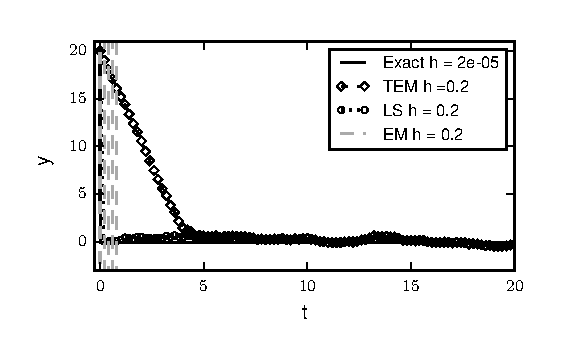
\includegraphics{papers/paperB/figures/ApplebyEx}
		\end{center}
		\caption{Likening between the EM, TEM and \SM approximations with unstable EM conditions. Here "exact" means
			a BEM solution with step size $h=\num{2e-5}$.}
		\label{fig:pathsAppleby}
	\end{figure}
\end{example}

\begin{example} We examine the \SM method using a SDE with super-linear grow diffusion. We 
	consider the SDE reported by \citeauthor*{Tretyakov2013} in \cite[Eq. (5.6)]{Tretyakov2013}
	\begin{equation}\label{eqn:SDETretyakov}
		dy(t) =
		\left(
			1-y^5(t) +y^3(t)  
		\right) dt
		+
		y^2(t) dW(t), \qquad y_0=0.
	\end{equation}
	\citeauthor{Tretyakov2013} show via simulation of \eqref{eqn:SDETretyakov} that the increment-tamed scheme
	\cite[Eq(1.5)]{Hutzenthaler2015}
	\begin{equation}\label{eqn:Increment-Tamed}
		X_{k+1} = X_k + 
		\frac{
			f(X_k) h + 
			g(X_k)\Delta W_k 
		}{
		\max\left(
		1, h
		\left|
		h f(X_k) +
		g(X_k)\Delta W_k
		\right|
	\right)}
	\end{equation}
	produces spurious oscillations. \citeauthor{Hutzenthaler2015} prove the convergence of this scheme under
	linear growth condition over diffusion. So, this suggests us that only certain kind of 
	explicit schemes with convergence under globally Lipschitz and linear growth diffusion conditions	
	%globally Lipschitz diffusion and linear growth 
	can extended their convergence to a locally Lipschitz diffusion and other kind of growth bound.
	Using $a(x):= -x^4 +x^2$, $b: = 1$ and $E=\{-1,0,1\}$, we construct the \SM method
	\begin{equation}\label{eqn:TreyakovLSMethod}
		Y_{k+1} = \exp(ha(Y_k))Y_k + 
		\frac{\exp(ha(Y_k)) - 1}{a(Y_k)} \1{E^c}
		+h\1{E}
		+Y_k^2\Delta W_k. 		
	\end{equation}
	\Cref{fig:Tretyakov} shows the numerical solution of SDE \eqref{eqn:SDETretyakov} with the Increment-Tamed (I-TEM) 
	\eqref{eqn:Increment-Tamed}, \SM method \eqref{eqn:TreyakovLSMethod}, and the Tamed (TEM) scheme. 
	We consider the implicit Midpoint scheme \cite[Eq.(5.3)]{Tretyakov2013} with $h=\num{e-4}$ 	as reference.
	\begin{figure}[h!]
		\centering
		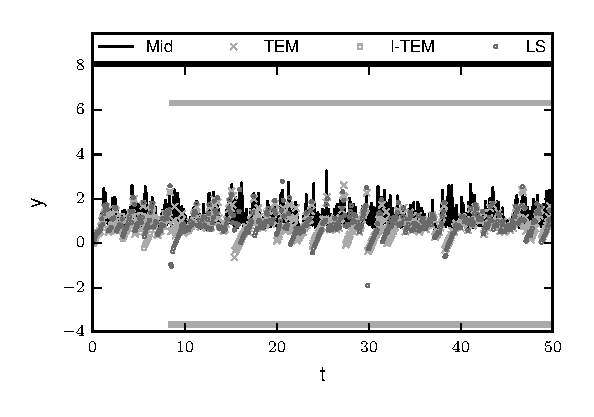
\includegraphics{./papers/paperB/figures/Tretyakov}
		\caption{
			Numerical solution of SDE \eqref{eqn:SDETretyakov} using the I-TEM 
			\eqref{eqn:Increment-Tamed}, \SM method \eqref{eqn:TreyakovLSMethod}  and TEM
			with $h=\num{0.1}$. The reference solution is a Midpoint rule approximation with $h=\num{e-4}$.
		}
		\label{fig:Tretyakov}
	\end{figure}
\end{example}

\begin{example}
	Now we compare the order of convergence and the run time of the \SM method with the TEM scheme as in 
	\cite{Hutzenthaler2012a}. That is, we consider a  Langevin equation under  the $d$-dimensional potential 
	$U(x)= \frac{1}{4}|x|^4 - \frac{1}{2}|x|^2$, and $d$-dimensional Brownian additive noise. The corresponding
	SDE reads
	\begin{equation}\label{eqn:SDELangevinHutz}
	dy(t) = 
		\left(
			y(t) - |y(t)| \cdot y(t)
		\right)dt
		+ dW(t), \qquad y(0)=0.
	\end{equation}
	This model describes the motion of a Brownian particle of unit mass immersed on the potential $U(x)$. 
	Taking $a_j(x):=1-|x|$ and $b_j=0$, $j\in \{1,\dots, d\}$ we obtain the \SM method
	\begin{equation}\label{eqn:LangevinLSMethod}
		Y_{k+1} = \diag
		\left[		
			e^{h a_1(Y_k)}, \dots, e^{ha_d(Y_k)}) 
		\right] 
		Y_k+
		\Delta W_k.
	\end{equation}
	\Cref{tbl:OrdersLS} shows the root means square errors at a final time $T=1$, which is approximated by
	\begin{equation}
		\sqrt{\EX{|Y_N - y(T)|^2}} \approx 
		\frac{1}{M}
		\left(
		\sum_{i=1}^M
		|y_i(T) - Y_{N,i}|^2	
		\right)^{1/2},
	\end{equation}
	over a sample of $M$ =\num{10000} trajectories of the TEM, \SM  and BEM solutions to SDE 
	\eqref{eqn:SDELangevinHutz} with dimension $d=10$.  We consider the TEM solution with step $h=2^{-19}$ as reference 
	solution. 
	In this experiment we confirm that the \SM method converges with standard order 1/2  and is almost equal accurate 
	as the TEM approximation.

		In some applicationa as in Browninan Dynamics Simulations \cite{Cruz2012}, the dimension of a SDE
	increases considerable the complexity and computational cost --- this excludes the use of implicit methods.
	In \Cref{fig:TimeVsDimension}, we observe that the runtime of the BEM method grows quadratically depending
	on the dimension, meanwhile the LS and TEM methods grow linearly. 
	\begin{table}[t]
		\centering
		\begin{tabular}{lllllll}
			&        TEM &        	& LS		&           & BEM		 &         \\
			\toprule
			h		& ms-error	 & ECO 		& ms-error	    & ECO		& ms-error	 &	ECO	  \\
			\midrule
			$2^{-2}$	& \num{1.70388}    & ---		&\num{1.55394}		& ---		& \num{1.38157}	& 
			--- \\
			$2^{-3}$	& \num{1.16977}    & \num{0.54}     &\num{1.10775}    & \num{0.48} & \num{1.05309}	& 
			\num{0.39} \\ 
			$2^{-7}$	&\num{0.27895}     & \num{0.48} & \num{0.27795}   & \num{0.48} & \num{0.276895}& 
			\num{0.48} \\
			$2^{-11}$	& \num{0.07010}  & \num{0.50} & \num{0.07009}  & \num{0.50} & \num{0.07007} & 
			\num{0.50} \\
			$2^{-15}$	& \num{0.01739}  & \num{0.51} & \num{0.01739}  & \num{0.51} & \num{0.01739}& 
			\num{0.51} \\
			\bottomrule
		\end{tabular}
		\caption{
			Mean square errors and the experimental convergence order (ECO) for the SDE \eqref{eqn:SDELangevinHutz} 
			with a TEM with $h = 2^{-19}$ as reference solution.
		}\label{tbl:OrdersLS}
	\end{table}
	\begin{figure}[t]
		\centering
			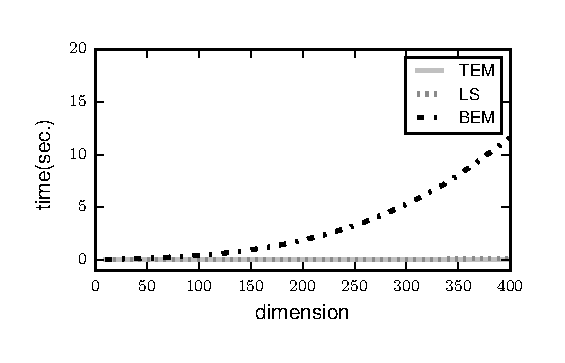
\includegraphics{./papers/paperB/figures/TimeVsDimension}
		\caption{
			Runtime calculation of $Y_N$ with $h=2^{-17}$, using the BEM,  \SM and TEM methods for 
			SDE \eqref{eqn:SDELangevinHutz}.
		}
		\label{fig:TimeVsDimension}
	\end{figure}
\end{example}

\begin{example}
	Let us recall the following  stochastic model for internal 
	HIV dynamics given by  \citeauthor{Dalal2008} in \cite{Dalal2008}:
	\begin{align}\label{eqn:StochasticHIVDynamics}
		dy_1(t) &=
		\left(
			\lambda -\delta y_1(t) - (1 - \gamma) \beta y_1(t) y_3(t)
		\right)dt
		-\sigma_1 y_1(t) dW^{(1)}_t, 
		\notag \\
		dy_2(t) &= 	
		\left(
			(1- \gamma) \beta y_1(t) y_3(t) - \alpha y_2(t) 
		\right)dt
		-\sigma_1 y_2(t) dW^{(1)}_t, 
		\\
		dy_3(t) & = 
		\left(
			(1 - \eta) N_0 \alpha y_2(t) 
				-\mu y_3(t)
			-(1 - \gamma ) \beta y_1(t) y_3(t) 
		\right)dt
		- \sigma_2 y_3(t) dW^{(2)}_t.
		\notag
	\end{align}	
	\begin{figure}[h!]
		\centering
		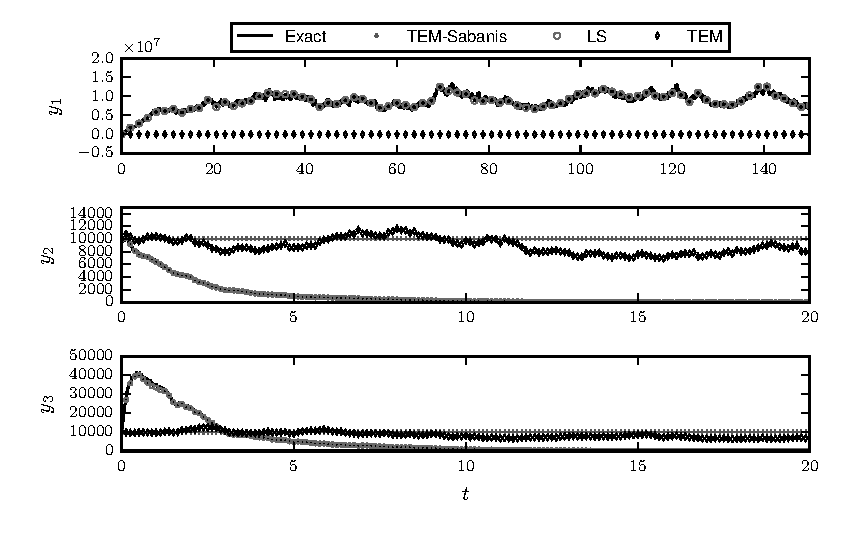
\includegraphics{./papers/paperB/figures/InternalHIVDynamics}
		\caption{
			Likening between EM, \SM, TEM approximations for SDE \eqref{eqn:StochasticHIVDynamics} with
			$\gamma = \num{0.5}$,
			$\eta = \num{0.5}$,
			$\lambda = \num{e6}$, 
			$\delta = \num{0.1}$,
			$\beta = \num{e-8}$,
			$\alpha = \num{0.5}$,
			$N_0= \num{100}$,
			$\mu = \num{5}$,
			$\sigma_1 = \num{0.1}$,
			$\sigma_2 = \num{0.1} $,
			$y_0 = (
			\num{10000},%{\per\cubic\deci\meter}, 
			\num{10000},%{\per\cubic\deci\meter}, 
			\num{10000}.%{\per\cubic\deci\meter}
			)^T$,
			$h=\num{0.125}$.
			Here the reference solution means a BEM simulation
			with the same parameters but with a step-size $h=\num{e-5}$.
		}
		\label{fig:InternalHIVDynamics5e-1}
	\end{figure} 
	Under certain conditions \citeauthor{Dalal2008} prove 
	that  system \eqref{eqn:StochasticHIVDynamics} has a unique 
	almost surely exponential stability solution, that is,  $y=(y_1,y_2,y_3)$  tends 
	exponentially to an equilibrium $(\bar{y}_1,0,0)$ with probability 1. 
	Now, we want to verify if  the EM, TEM, TEM-Sabanis \cite{Sabanis2015} and LS approximations can reproduce this 
	property of the solution. Taking 
	\begin{align*}
		E_1&:=\left\{
			(x,y,z)^T \in \R^3:
			z=0 
			\text{ or }
			z=0
			\frac{-\delta}{\beta(1-\gamma)}
		\right\}, \quad
		E_2:=	\emptyset,   \\
		E_3&:=\left\{
			(x,y,z)^T \in \R^3: 
			x=0
			\text{ or }
			x=
			\frac{-\mu}{\beta(1-\gamma)}
		\right\}
	\end{align*}
	 
	The LS method for \eqref{eqn:StochasticHIVDynamics} is given by
	
	\begin{align}
		a_{1}(Y_k)) &:= 
		-\left(
		\delta + (1 - \gamma) \beta Y_k^{(3)}
		\right),		
		& b_1(Y_k^{(-1)}) &:= \lambda, 
		& 
		\notag
		\\
		a_{2}(Y_k) &:= -\alpha,
		&b_2(Y_k^{(-2)}) & :=
		(1-\gamma) \beta Y_{k}^{(1)} Y_{k}^{(3)},
		\notag
		\\
		a_{3}(Y_k) &= 
		-
		\left(
		\mu + (1- \gamma) \beta Y_{k}^{(1)}
		\right),
		\qquad
		%
		&b_{3}(Y_k^{(-3)}) &:= 
		\left(
		1 - \eta 
		\right)
		N_0 \alpha Y_{k}^{(2)},
		\notag			
	\end{align}
	the \SM method for the stochastic model \eqref{eqn:StochasticHIVDynamics} reads,
	\begin{align}
		Y_{k+1} &= A^{(1)}(h,Y_k) \,Y_k + A^{(2)}(h,Y_k)b(Y_k)+ g(Y_k)\, \Delta W_k,
		\qquad \Delta W_k = \left(W_k^{(1)}, W_k^{(2)}\right)^T, 
		\notag\\ 
		A^{(1)}(h,Y_k)&:=
		\begin{pmatrix}
			e^{ha_1(Y_k)}	&	0	&0 \\
			0	&e^{ha_2(Y_k))}	&0\\
			0	&0				&e^{ha_3(Y_k))}
		\end{pmatrix},
		%	
		\notag
		\\
		%	
		A^{(2)}&:=
		\begin{pmatrix}
			h \Phi_1(Y_k)\1{E_1^c}	&0	&0\\
			0 & 
			\left(\displaystyle
			\frac{e^{-h\alpha} - 1}{\alpha}
			\right) & 0\\
			0 & 0 & h \Phi_3(Y_k)\1{E_3^c} 
		\end{pmatrix}
		%\notag \\
		+h
		\begin{pmatrix}
			\1{E_1}	&0 			&0\\
			0		&0			&0\\
			0		&0			&\1{E_3}\\
		\end{pmatrix},
	\notag
	\\
	b(Y_k) &:=
	\begin{pmatrix}
		b_1(Y_k^{(-1)})\\
		b_2(Y_k^{(-2)})\\
		b_3(Y_k^{(-3)})
	\end{pmatrix},
	\qquad
	g(Y_k):=
	\begin{pmatrix}
		-\sigma_1 Y_k^{(1)}	&0\\
		-\sigma_1 Y_k^{(2)}	&0\\
		0	&-\sigma_2 Y_k^{(3)}
	\end{pmatrix}.
\end{align}
%
	\Cref{fig:InternalHIVDynamics5e-1} shows the  \SM, TEM and TEM-Sabanis approximations
	with the parameters reported in \cite{Dalal2008}.  The EM approximation
	blows up  so it is not drawn. We observe how the TEM approximation (components $y_2$ and $y_3$) oscillates about 
	the initial condition and the 
	TEM-Sabanis approximation (components $y_2$ and $y_3$) is constant and equal to the initial value, while the \SM 
	method reproduces the asymptotic behaviour of the solution. It is important to remark that the Tamed family methods	
	improve convergence of the Euler method by taming the drift increment term with 
	the factor	$1/(1 + h |f(Y_k)|)$, bounding the norm of  $h f(Y_k)/(1 + h |f(Y_k)|)$ by 1. This norm   
	controls the drift contribution of the Tamed methods  at each step. Such modification 
	is recommended for SDEs with drift contributions and initial conditions with similar scales. We observe
	that for models where such terms have different scales the TEM over damps the drift contribution. 
\end{example}


	\chapter{Conclusions and future work}
		\label{ch:Chapter5}
		\section{Conclusions}
	We have constructed a new way  to design numerical methods for SDEs based on the Steklov average.
First we presented a scalar scheme  originated in an exact discretization for the deterministic version of the SDEs 
with desired stability properties --- the Steklov method.
We verified its convergence and stability over a standard globally Lipschitz setup and compared its performance with a 
competitive solvers.
%
Also, we have extended the explicit Steklov scheme for vector SDE by developing a new version based on a linearized 
Steklov average. This method is constructed on the basis that the drift function can be rewritten in the linearized 
form. Moreover, strong order one-half convergence has been proved for our explicit linear method and we have presented 
several applications formulated with the LS scheme. Finally, high-performance of the Linear Steklov method have been 
analyzed in diverse problems, even for SDEs with super-linear diffusion.
Future work will be focused on the following problems:
%
\begin{itemize}
	\item
		Numerical evidence suggests that the Steklov methods are suitable for SDEs with super-	
		linear growth diffusion. 
		So, one should prove this claim.
	\item
		Since we have proved strong convergence, we would to apply the Multilevel Monte Carlo 
		approach to
		the Brownian Dynamics Simulation using Steklov type schemes.		
	\item
		The schemes presented here have a simple structure like the	Euler-Maruyama family, so it 
		is possible	to formulate versions of the Tamed, Milstein, Balanced, Theta, 
		Runge-Kutta methods by approximating the drift term by its Steklov average.  
	\item	
		Also, it is viable to study stability of the LS method usibg the theory of random 
		dynamical systems.
	\item
		Furthermore, a natural extension of this work would be to design Steklov type schemes 
		for more general SDEs, that is, SDEs with delay, Poisson jumps or partial derivatives. 	
\end{itemize}

 
 
	
%backmatter
	\begin{appendices}
		\chapter{Useful Inequalities}
			In this appendix we enunciate basic results that are extensively used through our analysis. Here
the main reference are \cite{Shiryaev1996} and \cite{Mao2007}.
\begin{Holder}[{\cite[pg. 193]{Shiryaev1996}}]
	\begin{equation}\label{eqn:HolderInequality}
	\m[X^T Y] \leq
	\left(
	\m|X|^p
	\right)^{\frac{1}{p}}		
	\left(
	\m|X|^q
	\right)^{\frac{1}{q}}.
	\end{equation}
\end{Holder}

\begin{Young}[{\cite[pg. 111]{Hardy1934}}]
	\begin{equation}\label{eqn:YoungsInequality}
	|a||b| 
	\leq
	\frac{\delta}{p} |a|^p
	+\frac{\delta}{q \delta^{q/p}} |b|^q.
	\end{equation}
\end{Young}
%
\begin{Minkowski}[{\cite[pg. 194]{Shiryaev1996}}]
	\begin{equation}
	\left(
	\m |X+Y|^p
	\right)^{\frac{1}{p}}
	\leq
	\left(
	\m |X|^p
	\right)^{\frac{1}{p}}
	+
	\left(
	\m |Y|^p
	\right)^{\frac{1}{p}}.
	\end{equation}
\end{Minkowski}
%
%
\begin{Standard}
		Fix $1<p<\infty$ and consider a sequence of real numbers $\{a_i\}_{i=1}^{N}$  with $N \in \N$. Then one can 
	formulate this usefully inequality
	\begin{equation}\label{eqn:SingleHolder}
	\left(
	\sum_{j=1}^N a_j
	\right)^p
	\leq
	N^{p-1}
	\sum_{j=1}^{N}
	a_j^p.
	\end{equation}
\end{Standard}
%
\begin{Doobs}[{\cite[Thm. 3.5]{Mao2007}}]
%\begin{thm}[Doob's Martingale Inequality]
	Let $\{M_t\}_{t\geq 0}$ be a $\mathbb{R}^d$-valued martingale. Let $[a,b]$ be a bounded interval in $
	\mathbb{R}_{+}$.
	If $p>1$ and $M_t\in L^p(\Omega;\mathbb{R}^d)$ then
	\begin{equation}
	\label{eqn:DoobMartingaleInequality}
	\m\left( \sup_{a\leq t \leq b} |M_t|^p\right) 
	\leq \left(\frac{p}{p-1}\right)^p \m|M_b|^p. 
	\end{equation}
%\end{thm}
\end{Doobs}

\begin{bdg}[{\cite[Thm. 7.3]{Mao2007}}]
	Let $g\in \mathcal{L}(\mathbb{R}_+; \mathbb{R}^{d\times m})$. Define for $t\geq 0$
	\begin{equation}
		\label{thm:BDG}
		x(t) = \int_{0}^{t} g(s)dW(s) \quad \text{and } \qquad 
		A(t) = \int_{0}^{t} |g(s)|^2 ds.
	\end{equation}
	Then for all $p>0$, there exist universal positive constants $c_p$, $C_p$ such that
	\begin{equation}
		c_p\m|{A(t)}|^{\frac{p}{2}}
		\leq
		\m \left[
		\sup_{0\leq s \leq t} |x(s)|^p
		\right]
		\leq 
		C_p \m |A(t)|^{\frac{p}{2}},
	\end{equation}
	for all $t\geq 0$.  In particular, one may take
	\begin{align*}
	c_p &= (p/2)^p, & 			 C_p &= (32/p)^{\frac{p}{2}} & \text{if } 0<p<2; \\
	c_p &= 1,       & 			 C_p &= (32/p)^{\frac{p}{2}} & \text{if } p=2; \\
	c_p &= (2p)^{-\frac{p}{2}},& C_p &= \frac{p+1}{2(p-1)^{\frac{p}{2}}} & \text{if } p>2 .\\
	\end{align*}
\end{bdg}

\begin{Gronwall}[{\cite[Thm. 8.1]{Mao2007}}]
	Let $T > 0$ and $c \geq 0$. Let $u(\cdot)$ be a Borel measurable bounded nonnegative function on 
	$[0,T]$, and let $v$ be a nonnegative integrable function on $[0,T]$
	If
	$$
		u(t) \leq c 
		+\int_{0}^{t} v(s)u(s)ds \qquad \forall t \in [0,T],
	$$
	then
	\begin{equation}\label{thm:Gronwall}
		u(t) \leq c\exp
		\left(
		\int_{0}^{t} v(s)ds 
		\right)
		\qquad \forall t \in [0,T].
	\end{equation}
\end{Gronwall}
%
\begin{DiscreteGronwall}[{\cite[Lm. 3.4]{Mao2013}}]
	Let $M$ be a positive integer. Let $u_k$ and $v_k$ be non-negative numbers for $k=0,1,\dots,M$. 
	If
	$$
	u_k\leq u_0 + \sum_{j=0}^{k-1} u_j v_j
	$$
	then
	\begin{equation}
		\label{thm:DiscreteGronwall}
		u_k \leq u_0 
		\exp
		\left(
		\sum_{j=0}^{k-1}v_j
		\right).
	\end{equation}
\end{DiscreteGronwall}

	\end{appendices}
	%\cleardoublepage
	\addcontentsline{toc}{chapter}{References}
	\part*{References}
	\bibliographystyle{plainnat}
	\bibliography{bib/PhdThesisBib}
\end{document}